\pdfminorversion=4
\documentclass[letterpaper,12pt]{article}
\usepackage[top=1in, bottom=1in, left=1.25in, right=1.25in]{geometry}
\usepackage{setspace}
\setcounter{secnumdepth}{3} % this number depends on your depth of sections
\setcounter{tocdepth}{3} % this number should be equal to secnumdepth in previous
%\usepackage{subfigure}
%\usepackage[subfigure]{tocloft}
\usepackage{subcaption}
\usepackage{tocstyle}
\usepackage{mathtools}

\renewcommand{\contentsname}{\centerline {\normalsize\bfseries Table of Contents}}
\newtocstyle[standard][leaders]{mytocstyle}{\settocfeature[1]{entryhook}{\normalfont\bfseries}}
\usepackage[capposition=top]{floatrow}
\usepackage{listings}
\usepackage{cite}
\usepackage{esvect}
\usepackage{footnote}
\usetocstyle{mytocstyle}
\usepackage{sectsty}
\sectionfont{\normalsize\centering}
\subsectionfont{\normalsize}
\usepackage{enumitem}
\renewcommand{\thesection}{}
\renewcommand{\thesubsection}{\arabic{section}.\arabic{subsection}}
\usepackage{algorithm}
\usepackage{algorithm}
\usepackage[noend]{algpseudocode}
\usepackage{times}
\usepackage{latexsym}
\usepackage{graphicx}
\usepackage{cite}
\usepackage{balance}
\usepackage{multirow}
\usepackage{epstopdf}
\usepackage{threeparttable}
\usepackage[latin1]{inputenc}
\usepackage{amsmath}
\usepackage{amsfonts}
\usepackage{amssymb}
\usepackage{amsthm}
\usepackage{color}
\usepackage{xcolor}
%\usepackage{algorithm}
%\usepackage{algorithmic}
\graphicspath{ {images/} }
\usepackage{graphicx}
\usepackage{comment}
\usepackage{times}
\usepackage{cite}
\newtheorem{theorem}{Theorem}
\newtheorem{lemma}{Lemma}
\newtheorem{definition}{Definition}
\newenvironment{alginc}[1][pseudocode]{\medskip\algsetlanguage{#1}\begin{algorithmic}[1]}{\end{algorithmic}\medskip}
\newcommand{\Exp}{Exponential }
\newcommand{\G}{\mathbb{G}}
\newcommand{\Z}{\mathbb{Z}}
\newcommand{\PP}{Pairing }
\newcommand{\Gone}{\mathbb{G}_1}
\newcommand{\Gtwo}{\mathbb{G}_2}
\newcommand{\Gthree}{\mathbb{G}_3}
\newcommand{\Gt}{\mathbb{G}_T}
\newcommand{\PPo}{Pairing}
\DeclarePairedDelimiter{\ceil}{\lceil}{\rceil}
\DeclareMathOperator*{\argminA}{arg\,min} % Jan Hlavacek
\DeclareMathOperator*{\argminB}{argmin}   % Jan Hlavacek
\DeclareMathOperator*{\argminC}{\arg\min}   % rbp
\DeclareMathOperator*{\argmax}{argmax} 

\definecolor{lightgray}{rgb}{.9,.9,.9}
\definecolor{darkgray}{rgb}{.4,.4,.4}
\definecolor{purple}{rgb}{0.65, 0.12, 0.82}

\newtheorem{innercustomdfn}{Definition}
\newenvironment{customdfn}[1]
  {\renewcommand\theinnercustomdfn{#1}\innercustomdfn}
  {\endinnercustomdfn}

\lstdefinelanguage{JavaScript}{
    keywords={typeof, new, true, false, catch, function, return, null, catch, switch, var, if, in, while, do, else, case, break},
    keywordstyle=\color{blue}\bfseries,
    ndkeywords={class, export, boolean, throw, implements, import, this},
    %ndkeywordstyle=\color{darkgray}\bfseries,
    ndkeywordstyle=\color{green}\bfseries,
    identifierstyle=\color{black},
    sensitive=false,
    comment=[l]{//},
    morecomment=[s]{/*}{*/},
    commentstyle=\color{purple}\ttfamily,
    stringstyle=\color{blue}\ttfamily,
    morestring=[s]{`}{'},
%    morestring=[b]"
}

\lstset{
    language=JavaScript,
    backgroundcolor=\color{lightgray},
    extendedchars=true,
    basicstyle=\footnotesize\ttfamily,
    %basicstyle=\footnotesize\sffamily,
    showstringspaces=false,
    showspaces=false,
%    numbers=left,
%    numberstyle=\footnotesize,
%    numbersep=9pt,
    tabsize=2,
    breaklines=true,
    showtabs=false,
    captionpos=b
    emph={= },
    emphstyle=\color{green}
}

\lstset{
    language=JavaScript,
    backgroundcolor=\color{lightgray},
    extendedchars=true,
    basicstyle=\footnotesize\ttfamily,
    %basicstyle=\footnotesize\sffamily,
    showstringspaces=false,
    showspaces=false,
%    numbers=left,
%    numberstyle=\footnotesize,
%    numbersep=9pt,
    tabsize=2,
    breaklines=true,
    showtabs=false,
    captionpos=b
    emph={= },
    emphstyle=\color{green}
}

\colorlet{punct}{red!60!black}
\definecolor{background}{HTML}{EEEEEE}
\definecolor{delim}{RGB}{20,105,176}
\colorlet{numb}{magenta!60!black}

\lstdefinelanguage{json}{
    basicstyle=\normalfont\ttfamily,
    numbers=left,
    numberstyle=\scriptsize,
    stepnumber=1,
    numbersep=8pt,
    showstringspaces=false,
    breaklines=true,
    frame=lines,
    backgroundcolor=\color{background},
    literate=
     *{0}{{{\color{numb}0}}}{1}
      {1}{{{\color{numb}1}}}{1}
      {2}{{{\color{numb}2}}}{1}
      {3}{{{\color{numb}3}}}{1}
      {4}{{{\color{numb}4}}}{1}
      {5}{{{\color{numb}5}}}{1}
      {6}{{{\color{numb}6}}}{1}
      {7}{{{\color{numb}7}}}{1}
      {8}{{{\color{numb}8}}}{1}
      {9}{{{\color{numb}9}}}{1}
      {:}{{{\color{punct}{:}}}}{1}
      {,}{{{\color{punct}{,}}}}{1}
      {\{}{{{\color{delim}{\{}}}}{1}
      {\}}{{{\color{delim}{\}}}}}{1}
      {[}{{{\color{delim}{[}}}}{1}
      {]}{{{\color{delim}{]}}}}{1},
}

\usepackage[colorlinks=true,linkcolor=black,citecolor=red,urlcolor=red,plainpages=false,pdfpagelabels=true, bookmarks=false]{hyperref}
\begin{document}
   \author{{\normalsize Yinhao Xiao}}
   \title{\Large{\bf Security and Privacy of Smart Devices} \\ \large Dissertation}
   \date{}
   \maketitle
   \thispagestyle{empty}
   \begin{center}
       B.S. in Information and Computing Science,\\ May 2012, Guangdong University of Technology \\
       M.A. in Mathematics,\\ May 2014, The George Washington University \\
       M.S. in Computer Science,\\ Dec 2015, The George Washington University \\[\baselineskip]
       
       A Dissertation submitted to\\
       The Faculty of\\The School of Engineering and Applied Science\\ of The George
       Washington University\\ in partial satisfaction of the requirements\\ for the degree
       of Doctor of Philosophy\\[\baselineskip]
       March 8, 2018\\[\baselineskip]
       Dissertation directed by\\[\baselineskip]
       Xiuzhen Cheng\\Professor of Computer Science
   \end{center}
   % display page numbers in the footer and centered. Start with roman numerals %
   \pagestyle{plain}
   \setcounter{page}{1}
   \pagenumbering{roman}


   \newpage
   \doublespacing
   \begin{center}
   {\Large{\bf Security and Privacy of Smart Devices}\\ \large Dissertation}\\[\baselineskip]
   {\normalsize Yinhao Xiao}
   \end{center}
   \noindent Dissertation Committee:\\

   \hfill\begin{minipage}{5in}
   {Xiuzhen Cheng, Professor of Computer Science, Dissertation
       Director}\\[\baselineskip]
  {Hyeong-Ah Choi, Professor of Computer Engineering, Committee Member}\\[\baselineskip]
  {Arkady Yerukhimovich, Assistant Professor of Computer Science, Committee Member}\\[\baselineskip]
   {Xiang Chen, Assistant Professor of Computer Engineering, Committee Member}\\[\baselineskip]

   
   
   \end{minipage}

   \newpage
      \section{Abstract}
   The advent of smart devices, i.e., smartphones and smart home devices, has greatly revolutionized and modernize people's daily lives in every aspect. Yet, the security condition of the devices and their corresponding systems is concerning since traditional security measures fail to cope with them due to limitations of computation power and hardware/firmware heterogeneity. In this dissertation, we present our research on studying the security and privacy issues of smartphones and of smart home devices.
   
   Firstly, we study the OS security of Android devices. In order to facilitate apps to collaborate to finish complex jobs, Android allows isolated apps to communicate through explicit interfaces. However, the communication mechanisms often give additional privilege to apps, which can be exploited by attackers. The Android Task Structure is a widely-used mechanism to facilitate apps' collaboration. Recent research has identified attacks to the mechanism, allowing attackers to spoof UIs in Android. In this work, we present an analysis of the security of the Android task structure. In particular, we analyze the system/app conditions that can cause the task mechanism to leak privilege. Furthermore, we identify new end-to-end attacks that enable attackers to {\em actively} interfere with victim apps to steal sensitive information. Based on our findings, we also develop a task interference checking app for exploits of the Android task structure.
   
    Secondly, we study how the side-channel information publicly available in Android devices can result in severe privacy leakage on social networks. Owing to the various features provided by mobile devices, a user's online social activities are tightly tied to his phone, and are conveniently, sometimes unnecessarily, available to social networks. In this work, we propose a novel attack architecture to show that attackers can infer a user's social network identities behind a mobile device through new dimensions. Specifically, we first developed a correlation between a user's device system states and the social network events, which leverage multiple mechanisms such as learning-based memory regression model, to infer the possible accounts of the user in the social network app. Then we exploited the social network to social network correlation, via which we correlated information across different social networks, to identify the accounts of the target user. We implemented and evaluated these attacks on three popular social networks, and the results corroborate the effectiveness of our design.
    
    Thirdly, we explore the defense mechanisms on strengthening the smart home systems. Smart home systems have become more and more prevailing in recent years. On one hand, they greatly convenience our everyday lives; on the other hand, they suffer from the two notorious security problems, namely the open-port problem and the overprivilege problem, making their security situations extremely worrying and uncheerful. In this work, we proposed a novel credential-less authentication framework, CLAF, to effectively defend against the attacks resulted from these two security problems without the need for sensitive credentials. We further detailed an implementation of CLAF based on the side channels that are publicly available in Android smartphones serving as controllers of smart home systems and presented its workflow in protecting against various attacks caused by the open-port and overprivilege problems. Finally, we tested our CLAF implementation on a real-world smart home system and considered four threat models that cover basically all practical attacks, including Mirai and its variants. We also considered the effectiveness of our CLAF implementation on the SmartApps of the Samsung SmartThings platform, which suffers from the open-port and overprivilege problems. The evaluation results indicate that our CLAF realization can successfully defend against over 90\% attack trials with an average latency less than 1 second.
    
   
      \newpage

   \newgeometry{top=1in, bottom=1in, left=1.125in, right=1.125in}
   \tableofcontents
   \restoregeometry
   \newpage


   \cleardoublepage
   \phantomsection \label{listoffig}
   \addcontentsline{toc}{section}{\hspace{1.5pt} List of Figures}
   \begin{center}
       \listoffigures
   \end{center}
   \newpage
   
   \cleardoublepage
   \phantomsection \label{listoftbl}
   \addcontentsline{toc}{section}{\hspace{1.5pt} List of Tables}
   \begin{center}
       \listoftables
   \end{center}
   \newpage


   \newpage
   \setcounter{page}{1}
   \setcounter{section}{1}
   \pagenumbering{arabic}
   \begin{singlespace}
       \section{Introduction}
   \end{singlespace}
   \setcounter{section}{1}
   \doublespacing
Smart devices refer to the electronic devices that are connected to the cloud or edge servers or with each other through different wireless protocols (e.g., Wi-Fi, 4/5G, Zigbee, Bluetooth, Software-Defined Radio, RFID, etc) in order to complete ubiquitous ``smart'' tasks such as sensing, controlling, actuating, messaging, or even decision making. Smart devices can mainly be taxonomized into two categories: smart mobile devices (i.e., smartphones and tablets), and smart home devices (e.g., smart thermostats, smart light, smart switch, and smart speakers). According to market research conducted by Statista, the total revenue of the smart devices in the US has reached 79.8 billion dollars by the year 2018~\cite{Statista:smarthome}\cite{statista:smartphone}. It is also projected that the average number of networked smart devices per person can reach 13 by the year of 2021~\cite{smartdeviceperperson}.

With the presence of the prevailing performance with respect to market sharing, as shown above, one may raise a question: If security vulnerabilities of smart devices and their corresponding systems are discovered by vicious personnel who later exploits these vulnerabilities to conduct malicious activities, are the consequences more serious than the ones of traditional computer or Internet infrastructure? Unfortunately, the answer is positive for this question due to the following two reasons:
\begin{itemize}
\item Smart devices tend to reflect more personal information than the tradition computers do. For example, using smartphones to take pictures has become the main way of photo-taking\cite{smartphonephoto}. Hence, the smartphone is the major source to store a user's personal photos. It is not difficult to envision the devastating consequence if an attacker can access the resources in a smartphone without authorization through security breaches.

\item Smart devices are interconnected tightly for better functioning and automation (e.g., a smart home system). The security drawback of the design allows an attacker to take down the whole system more quickly and effectively by compromising a single device, to begin with. A notable example is the Mirai virus which managed to infect 200,000 -
300,000 IoT smart devices in the first 20 hours~\cite{antonakakis2018mirai}.
\end{itemize}

Even though defending smart devices against malicious exploits and attacks is urgent and critical, securing them is more challenging than securing traditional computers not only because they are computationally limited to empower high-end firewalls, but are highly heterogeneous both on the hardware level and firmware level. Having observed the situation,  we mainly focus on identifying vulnerabilities, inventing attacks, and developing corresponding defensive mechanisms for smart devices. In this dissertation, we specifically target the security of smartphones and their corresponding systems. In the following contexts, we focus on two main directions of studying the security and privacy of smartphones, i.e., from the perspective of system design flaw and from the perspective of side-channel information exploit. For the system design flaw, we mainly present an OS level logic flaw existing in Android Task Mechanism that results in severe privilege leakage, through which we implemented four proof-of-concept attacks. Lastly, we developed an efficient scanner to help users to avoid the attacks. For the side-channel information exploit, we mainly present a novel attack vector which effectively associates the user's identity in social networks with the smartphone device using Android side-channel information. In addition, we also identify the security and privacy issues existing in a most typical smart home environment. We then propose a novel security framework for securing the smart home system from being affected by the most prevailing attacks in the real world.

\subsection{Exploiting Android Task Mechanism}
The Android system's security is based on several layers of security
mechanisms. In particular, each app is assigned a set of permissions and is only allowed to access system resources and services within the
permissions given. In addition, to prevent apps from accessing
information of others, each app is confined into its own partition.
It is enforced using the process isolation and user-based protection
mechanisms provided by Linux, where each app is assigned to a unique
Linux user ID.

Strong isolation increases the bar for attackers to carry out
malicious activities, but it also hinders benign apps from
communicating and collaborating with one another. To facilitate apps
collaboration in a complex task, Android allows isolated apps to
communicate through explicit interfaces, such as the Intent
mechanism. For example, Instagram uses intents to access the Single
Sign-On (SSO) service of Facebook to authenticate users.  Furthermore,
Android provides the Android Task Structure mechanism to allow activities
from different apps to be seamlessly integrated into a task, giving
them convenience when accessing common information. For example,
when Instagram uses the Facebook API for the authentication service
provided by Facebook, users can navigate through activities Instagram
app and Facebook app as if they are the same app.

Though the mechanisms are designed for facilitating app communication
and collaboration, relaxing the isolation provided by the Android
system often causes over-permissive privilege to apps. 
As the task mechanism of Android is developed to facilitate inter-app
collaboration, apps in a task may get additional privilege beyond what
is allowed by the isolation-based Android security
mechanism. Demonstrated by recent exploits~\cite{TaskHijacking}, a
malicious app can hijack the task mechanism for attacks such as
spoofing and phishing. The privilege obtained by apps in the same task
is well beyond that for collaboration, effectively making the Android
task mechanism a form of authorization.

In this work, we conduct an analysis of the security of the Android
task mechanism. First, we analyze possible ways that an app can join a task
and the privilege ``leaked'' to other apps in the same
task. Specifically, to explore the ways Android controls tasks, we
dynamically probe possible combinations of the flags and system states
that can affect an app's task status.  We also analyze the additional
privilege that can be obtained by an app when it joins a task. Second, built on the understanding of the task control mechanism and task privileges, we identify end-to-end attacks that steal information from other apps. In particular, we identified four proof-of-concept attacks based on exploiting the task mechanisms. The attacks include
UI phishing, screenshot based password stealing, activity-in-the-middle
activity, and gallery stealing. All of them only require common
permissions, e.g., \texttt{INTERNET} and \texttt{READ\_EXTERNAL\_STROAGE}. Compared to
the attacks by existing exploits, we have identified new attack
mechanisms that can {\em actively} interfere with benign apps. The
short video demos can be found in~\cite{demo}. Finally, to prevent attackers from misusing the task mechanism, we develop an efficient scanner that can help users to
identify the risks related to Android tasks.

The details of this work are presented in Section~\ref{sec:atmtitle}. 

\subsection{Device-Identity Association Attack Using Android Side-Channel Information}
Online social networks such as Twitter and Flickr revolutionize the ways people interact with each other. More and more users begin to access social networks through mobile devices, making it completely possible to de-anonymize a target individual based on the side-channel information from his mobile device due to the rich features generated by the user's device while operating on social network apps. We call this kind of attack \emph{device-identity association}. Though it is relatively difficult for an attacker to trick users into installing malware with strong permissions, recent research shows that public information obtained from the Android system without permission can be used to link to a user's identity \cite{zhou2013identity}. Nevertheless, the attack method proposed in \cite{zhou2013identity} by observing the fixed TCP payload sequence pattern is no longer effective due to the recent updates of the social network apps. We manually monitored the Twitter app's TCP sequence while tweeting and found that the sequence was irregular and noisy. Then we used Frida, an injection framework~\cite{frida}, to trace the function calls of the Twitter app, and found that the root cause lies in that the Twitter app no longer handles each tweeting event in a separate TLS session (separate calls to the \texttt{url.openConnection()} function), but rather combining them into one TLS session (only one call to the \texttt{url.openConnection()} function).

We also observed that the attack based solely on the mobile device side-channels faces challenges due to limited information from one social network app. Nevertheless, in practice, the majority of social network users access their accounts very infrequently, according to our study on 500,008 Twitter accounts); and a user typically has accounts in different social networks such as Twitter, Flickr, and Instagram; furthermore, the social network accounts of the same user are often highly similar/correlated in their user profiles, e.g., user name, picture, and locations. Such facts reveal a high potential of device-identity association based on account correlations. 

The objective of this work is to investigate efficient and effective techniques to accurately identify a target user (more precisely, the social network accounts of the user) in social networks even though the information obtained by an attacker is limited. 
In order to accomplish this goal, we proposed a novel attack architecture with two attack vectors, correlation from device system states to a social network (DS-SN) and correlation for cross social networks (SN-SN). For the DS-SN attack, we studied the association between a user's identity in a social network and the user's device system states, e.g., memory and network data. In our threat model, an attacker can get information from the system level of a user's smartphone through installed apps without any permission or the user's consent. Leveraging these states, the attacker can infer the system events, e.g., activity transitions and keyboard status, which can be used to further infer the user's social network events, e.g., sending tweets and posting Instagram photos at certain timestamps. The attacker then collects and aggregates these social network events to identify the target user's identity in the social network. However, DS-SN is sometimes not enough to identify a user's identity due to limited social network events the user leaves in a single social network; therefore, we proposed the idea of SN-SN attack, which exploits the cross social network similarity to allow the attacker to efficiently and accurately figure out the identities of a user through the system and network state left by the user's activities and account profiles on the social networks. 

The details of this work are presented in Section~\ref{sec:dssnassociate}. 

\subsection{Strengthening Security for Smart Home Systems}
Smart home systems, also known as home automation systems, represent a class of the most prevailing applications of the Internet of Things (IoT) in the physical world. They have significantly revolutionized the lifestyles of human beings from every aspect. The emerging market for smart home systems and devices has been growing rapidly. According to a recent statistical study, the revenue of the global smart home market has reached 31.4 billion US dollars by the year 2018 and is projected to reach 53.45 US dollars by the year 2022~\cite{smarthomemarket}. 

Even though the market for smart home systems has been prospering in recent years, their security condition is not cheerful. Current designs of smart home systems suffer from two major security problems, namely the \emph{open-port} problem and the \emph{overprivilege} problem. The open-port problem refers to that some smart home devices open certain TCP/UDP ports allowing any entity who has the Internet access, besides the authorized users, to directly communicate with them through the open ports. For examples, we observed that the Google Home Speaker opens port 8008 which accepts multiple commands such as \emph{scan available ambient Wi-Fi access points} and \emph{return the scan results unconditionally} without any credential, and that the smart switches produced by Wemo, one of the best-selling smart home brands on Amazon~\cite{bestselling}, open port 49153 which allows anyone to turn on/off the devices with no verification at all. Such an open-port problem is also the root cause of the wide prevalence of Mirai and its variants~\cite{antonakakis2017understanding}, which infected more than 65,000 devices within the first 20 hours of its first occurrence in 2016. The overprivilege problem refers to that a smart home app intentionally acquires excessive privileges or is passively assigned unnecessary privileges, which can allow a malicious app to perform operations against the user's will. For example, an overprivileged app that is only intended to control a smart light is granted the privilege of being able to unlock a user's door lock. 

These two security problems are the direct consequences of the design philosophies of IoT: pervasive connections and light-weight protocols; thus it is almost impossible to completely solve them in the foreseeable future, even though researchers have been making signs of progress to mitigate them. Nevertheless, the seriousness and impact broadness of these two security problems are huge, as demonstrated by our case studies reported in Section~\ref{sec:preliminaries}. Unfortunately, traditional credential-based mechanisms that have been successfully adopted by computer and Internet systems cannot be directly applied in smart home systems since they require the smart home devices to more or less store a user's credentials, i.e., the user's account information. However, such a measure can impose new security threats since smart home devices are computationally weak at both hardware and software levels leaving the devices more vulnerable to attacks. The possibility of compromising a smart home device is way easier than compromising a powerful backend server such as Amazon EC2, exposing users to higher risks of credential leakages.

In this study, we provide a mechanism that does not require any credential, to defend against the two security problems. Note that we do not target mitigating the two problems as they are rooted from the fundamental designs of the IoT devices and systems; instead, we aim to design a mechanism that can provide a \emph{cage} to confine the bad consequences caused by the two problems to the best/maximum extent: even though the port of a device is open and/or its app is overprivileged, the device or its app cannot do anything bad within the cage. Based on this consideration, we propose CLAF, a novel Credential-Less Authentication Framework serving as a defense wall to effectively control the access to the open ports of smart home devices and restrict the access rights of the overprivileged smart home apps. CLAF consists of three main components: (1) an evidence provider which collects \textit{evidence} proving that an operation is indeed performed by an authorized smart home app; (2) an operation handler which filters or passes an incoming operation based on a list of user-defined \textit{policies}; and (3) a policy server located on a secure backend system to store the \textit{policies} that clearly specify \emph{who can do what by how}. 
We further compare CLAF with the two recently proposed patching-based mechanisms to defend against the overprivilege problem in smart home systems, namely ContexIoT~\cite{jia2017contexiot} and SmartAuth~\cite{tian2017smartauth}, and claim that CLAF not only can provide the same protection against the overprivilege problem but also can inhibit attack cases these two mechanisms fail to defend. While CLAF is a general framework which allows a group of solutions, we provide an implementation with the evidence provider running on a user's smartphone as a mobile app without the need of rooting nor requesting for any sensitive permissions, the operation handler running on the user's gateway to provide maximized protection effect, and the policy server running on the Samsung SmartThings platform that supports a large number of smart home devices. Our solution does not need any patching to pre-programmed codes by the smart home manufacturers. We evaluate our framework and solution based on two sets of experimental environments: (1) a real-world typical smart home system with most of the popular smart home devices configured, considering four threat models that basically cover all practical attacks as well as the most notorious IoT-specific Mirai and its variants as attack vectors, and (2) 137 and 68  SmartApps on the Samsung SmartThings platform to respectively study the open-port problem and the overprivilege problem. For both experimental environments, our CLAF implementation can defend against all attack trials with more than 90\% success rates. The average latency produced by adopting our solution is less than \emph{1} second. 

The details of this work are presented in Section~\ref{sec:claf}. 

   \newpage
      \begin{singlespace}
           \section{Preliminaries}
      \end{singlespace}
   \label{sec:preliminaries}
\subsection{Android Security Basis and Android Task Mechanism}
Components in Android include {\em Activity}, {\em Service}, {\em
  Content Provider}, and {\em Broadcast Receiver}. An activity,
representing a single screen with user interface, is the most basic
elements in Android OS. A service in Android is a UI-less component
running in the background. A content provider supplies data from one
application to another through methods of the \texttt{ContentResolver}
class with the ways of storing data in databases, in files, or over
the network. A broadcast receiver responds to broadcast messages from
other applications.

Android adopts several layers of isolation and sandboxing mechanism as
its basic mechanism of security. In particular, it defines a set of
permissions to control the access of apps. Apps can access specific
resources only if they are granted with required permission.  In
addition, Android uses user-based protection of Linux to isolate
apps. It allocates a unique Linux user ID to each app, which naturally
isolates the app from others using the process-based isolation
mechanism provided by the Linux kernel.

The Android task mechanism is designed for facilitate inter-app
communication and for better support app collaborating under same
tasks. It allows activities from different apps can reside in the same
task to perform communications more conveniently~\cite{taskdoc}.  As
an example, when the user clicks a ``feedback'' button from an
activity of a game app, Android starts the composer activity of an
email app, and puts it onto the game app's activity.  After the user
finishes sending email, the composer activity is put off and the game
app returns to the top.  In such a way, two activities are organized
to finish a task, while they are actually from different apps.


The Android task mechanism is affected by several flags of apps. The
following are the key attributes affecting how apps are grouped.

\textbf{launchMode:} This is the attribute which decides how an activity
will be launched. It has four values, i.e., \textit{standard},
\textit{singleTop}, \textit{singleTask} and
\textit{singleInstance}. Activities with \textit{standard} or
\textit{singleTop} can be instantiated multiple times while activities
with \textit{singleTask} or \textit{singleInstance} can only begin a
task and be the root of the task. Moreover, \textit{singleInstance}
does not permit other activities to be part of its task. An
activity without \textit{launchMode} specifically set is
assumed to be \textit{standard} by default.

\textbf{taskAffinity:} Activities with the same \textit{taskAffinity},
normally the name of the package, conceptually are in the same task,
but this is not always the case. We refer to
Section~\ref{sec:atmapproach} and Table~\ref{tbl:taskinterference} for
more details. An activity without this attribute set is assumed to
have the same \textit{taskAffinity} as its own package name.

\textbf{allowTaskReparenting:} This is a boolean attribute indicating
whether an activity can be moved to the task which has the same
\textit{taskAffinity} from the original task it is started. An
activity without this attribute specifically set is assumed to be
\emph{allowTaskReparenting=false}.

For better demonstration, consider the example where an app has the
functionalities of viewing contacts as well as sending emails to
contacts. The app has two activities for these two functionalities,
\textit{SendEmailActivity} and \textit{ViewContactActivity}. For
better IPC and logic concerns, designers of the app set the
\textit{taskAffinity} of \textit{SendEmailActivity} to be the same as
the system email app, the \textit{taskAffinity} of
\textit{ViewContactActivity} to be the same as system contact app and
\textit{allowTaskReparenting} to be true for both activities.

\subsection{Publicly Available System States in Android}
In this subsection, we present the publicly available side-channel state information in Android that are exploited by our proposed inference attacks detailed in Section~\ref{sec:dssnassociate}. We focus on three common channels of public information, namely memory, CPU, and network.

\subsubsection{Memory}
The Android system leverages Android Runtime (ART) or its predecessor, Dalvik Virtual Machine (DVM), as the runtime environment to execute binaries in the Dalvik Executable (DEX) format. Both ART and DVM use the paging and memory-mapping mechanisms \cite{androidmemoverview} to manage memory allocation of apps. Particularly, Android maintains four types of memory data for each process running on the system: \texttt{Virtual Set Size} (\emph{VSS}), \texttt{Resident Set Size} (\emph{RSS}), \texttt{Proportional Set Size} (\emph{PSS}), and \texttt{Unique Set Size} (\emph{USS}), which are listed in Table~\ref{tab:memory}.

\begin{table}[h]
\centering
    \caption{Memory Size Information}
\begin{tabular}{|l|p{4.5cm}|}
    \hline\hline 
    \textbf{Type of Memory Size} & \textbf{Description} \\ 
    \hline\hline 
    \small Virtual Set Size (VSS) & \small Total virtual memory of a process \\ 
    \hline 
    \small Resident Set Size (RSS) & \small Total physical memory of a process \\ 
    \hline 
    \small Proportional Set Size (PSS) & \small Memory shared between a process and other processes \\ 
    \hline 
    \small Unique Set Size (USS) & \small  The set of pages unique to a process\\ 
    \hline 

\end{tabular} 
        \label{tab:memory}
\end{table}

Android does not treat memory information as sensitive
system data. Consequently, an app can obtain other apps' memory
information without requesting any permission. There are four methods to retrieve
the memory data of an app, which are listed below:
%
\begin{itemize}
\item The Android API has a standard class \texttt{Debug.MemoryInfo},
  which provides complete interfaces to query the information for
  a process~\cite{apimem}, including private dirty pages, shared dirty
  pages, and the PSS for Dalvik.
\item The \texttt{/proc} file system has \texttt{/proc/pid/statm}
  (\texttt{pid} is the id of the process) that lists all four types of
  memory information: \emph{VSS}, \emph{USS}, \emph{RSS}, and \emph{PSS}.
\item The commands ``\texttt{top}'' and ``\texttt{ps}'' in Android
  Toolbox~\cite{toolbox} yield \emph{VSS} and \emph{RSS} for any given
  process. These commands also use information from the \texttt{/proc}
  file system.
\item In some devices, \texttt{/system/xbin/procrank} is provided.
  The command \texttt{procrank} yields all four types of memory
  information for all processes in real time.
\end{itemize}

\subsubsection{CPU Usage}
Android maintains three types of CPU usage data for a process, which are publicly available:
%
\begin{itemize}
\item CPU usage rate: the total percentage of time a
  CPU operates on a running process, with 100\% indicating that for a given period,
  the CPU spends all its available cycles running the specific process.

\item User time (\texttt{utime}): the CPU time spent in the user code of a process, measured in clock ticks.

\item System time (\texttt{stime}): the CPU time spent in the system code (which is
  the kernel) of a process, measured in clock ticks.

\end{itemize}

A zero-permission app can retrieve the CPU usage data of
another app by either (1) accessing \texttt{/proc/pid/stat} which lists
\textit{user time}, \textit{system time}, and other time-related information; or
(2) using commands ``\texttt{top}'' and ``\texttt{ps}'' with Android
Toolbox to return the user time, system time, and CPU usage percentage
of any given process.

\subsubsection{Network}
Android does not store the contents of TCP packets of any
process; but it maintains a record of the number of bytes sent and received through TCP connections by a process. This information is available to any
zero-permission app, and can be obtained by the following
ways:
\begin{itemize}
\item The \texttt{TrafficStats} from Android API has the method
  \texttt{getUidRxBytes(int uid)}, which returns the received bytes for a
  given user ID \texttt{uid}.

\item The \texttt{/proc} system files
  \texttt{/proc/uid\_stat/pid/tcp\_snd} and \\
  \texttt{/proc/uid\_stat/pid/tcp\_rcv} respectively maintain the bytes sent and
  received for an app.
\end{itemize}

\subsection{Preliminary Study of the Security Conditions on Smart Home Systems}
In this subsection, we present two case studies to demonstrate the impact broadness of the open-port problem, summarize the prior research results to show the severity of the overprivilege problem.

We noticed that in order for a smart home device to accept a command without verification, the device must have an open port accepting messages and this open port does not verify whether or not the message is from an authorized source. Having identified these two features, we built a static and automatic binary analyzer based on the Angr framework~\cite{shoshitaishvili2016state}\cite{stephens2016driller}\cite{shoshitaishvili2015firmalice}, which parses the control-flow graph (CFG) of a given firmware and conducts breadth-first search (BFS) over the CFG to check if system calls to \texttt{socket}, \texttt{bind}, \texttt{listen}, \texttt{accept}, and \texttt{recv/read} exist in a descending order since they are the determining factors to tell whether the given firmware opens a port. Then our analyzer tracks if there are conditional jumps in the contents retrieved from \texttt{recv/read} over sensitive terms such as ``password'', ``token'', ``authorization'', etc, to check if the firmware has an authentication mechanism. We collected 2,905 embedded firmwares by crawling from the firmware databases of popular smart home brands such as Xiaomi, DLINK, TP-LINK, and Wemo, as well as from the database collected by Costin \emph{et al.}~\cite{costin2014large}. Each firmware is associated with \emph{one type} of device. Then we fed these firmwares to our analyzer. Our results indicate that in total 1,541 (53.03\%) firmwares suffer from the open-port problem, i.e., having ports publicly open to accept operations without authentication. Note that whether these ports are open-to-LAN or open-to-public is determined by the ways according to which these devices are configured for network connection: if a device is assigned with a public IP, the ports of the device are open-to-public; if it is configured under a LAN, the ports are open-to-LAN. 

We also studied the publicly accessible devices from the database collected by Shodan, the world's first and largest search engine for Internet-connected devices, via the Shodan API~\cite{matherly2009shodan}. We examined the latest Shodan database~\cite{shodannews}, which was updated on June 15, 2017, and found that at least 16,568,788 devices are publicly accessible through the Internet. By further restricting the devices to smart home systems, we observed that at least 731,331 smart home devices can be accessed through the Internet, which means that each of these devices has a public IP address and has at least one port widely open to the public. Among all these smart home devices, the most affected type is camera, with 350,516 (47.93\%) devices being publicly accessible, followed by smart switches, with the number being 135,261 (18.50\%). We also found that the total number of ports 80, 8080, 8081, 10000, and 49153 accounts for 51\% of all the open ports. Since the open ports require no authentication or verification to be accessed, the numbers mentioned above imply that many devices can be easily taken control by a remote attacker who only needs to send a control command through the Internet. This explains why the most notorious IoT viruses, Mirai and its variants, can quickly infect a large number of devices after their first occurrences. Note that the devices under this study are all open-to-public.

The overprivilege problem has been attracting much attention in smart home systems in recent years. According to the study by Fernandes \emph{et al.}~\cite{fernandes2016security}, 55\% of the 521 SmartApps on the Samsung SmartThings platform were significantly overprivileged. After Samsung removed the reported overprivileged SmartApps, 16.7\% of the remaining ones still have the overprivilege issue.  Researchers also found that the Amazon Echo has a design flaw which results in an overprivilege issue that allows an app to secretly record a user's speech~\cite{amazonoverprivilege}. Google Home Speaker has a similar overprivilege issue, via which a malicious app can eavesdrop a user's speech~\cite{googleoverprivilege}. Smartphones play an important role in smart home systems; nevertheless, it was reported that over one-third of the smartphone apps in the Android system are overprivileged \cite{felt2011android}. 

One can see from the above studies that the two security problems have a broad impact on the current smart home systems and can significantly threaten the users' security and privacy. As a matter of fact, the most famous DDoS attack on IoT, the Mirai Botnet, which exploits the open-port problem, is still committing atrocities to infect massive amount of IoT devices connected to the Internet nowadays.


   \newpage
   \begin{singlespace}
   \section{Privilege Leakage and Information Stealing through the Android Task Mechanism}
   \end{singlespace}
    \label{sec:atmtitle}



%===============================================================================

\subsection{Threat Model and Approach Overview} \label{sec:threatandapproach}

In this subsection, we present the threat model and the overview of our attack approach.

\subsubsection{Threat Model} \label{subsec:threat}

To study the security of the Android task mechanism, we consider a
scenario as follows. There are two apps, i.e., AppB and AppM,
installed in the same Android device, where AppB is benign and AppM is
developed by attackers.  We assume AppM does not have to require any
permission to manipulate tasks. However, we assume AppM can be granted
permissions for following-up behaviors, such as sending the retrieved
information out or accessing local storage.

\subsubsection{Approach Overview} \label{sec:approachoverview}

The goal of our work is to comprehensively analyze the Android task
mechanism to identify attacks, as well as creating solutions to
prevent such attacks.

As shown in Figure~\ref{fig:arch}, our research consists of four
components: \textsl{Understanding Task Control}, \textsl{Understanding
  Task Privilege}, \textsl{Exploitation Analysis} and \textsl{Task
  Interference Checking}.

The first component is to analyze the Android task mechanism,
identifying control conditions that can be leveraged by attackers.
We aim to find out the interference of tasks between two
apps, and identify the dominating factors deciding the apps'
property.  Secondly, we focus on studying the additional privilege
apps obtained when two apps are in the same task. We delicately test sensitive
system APIs and compare the difference of the results before and after
apps in the same task. Based on the understanding from the previous
stages, to demonstrate the achievability and severity of the
privilege escalation against Android task mechanism, we develop four light-weight
real-world attacks that can steal the sensitive information
successfully, most of which only requires \texttt{INTERNET}
permission.  At last, we design a task interference checking app to
detect the task interference between users' important apps and other
installed apps.

\begin{figure*}[t]
        \centering
        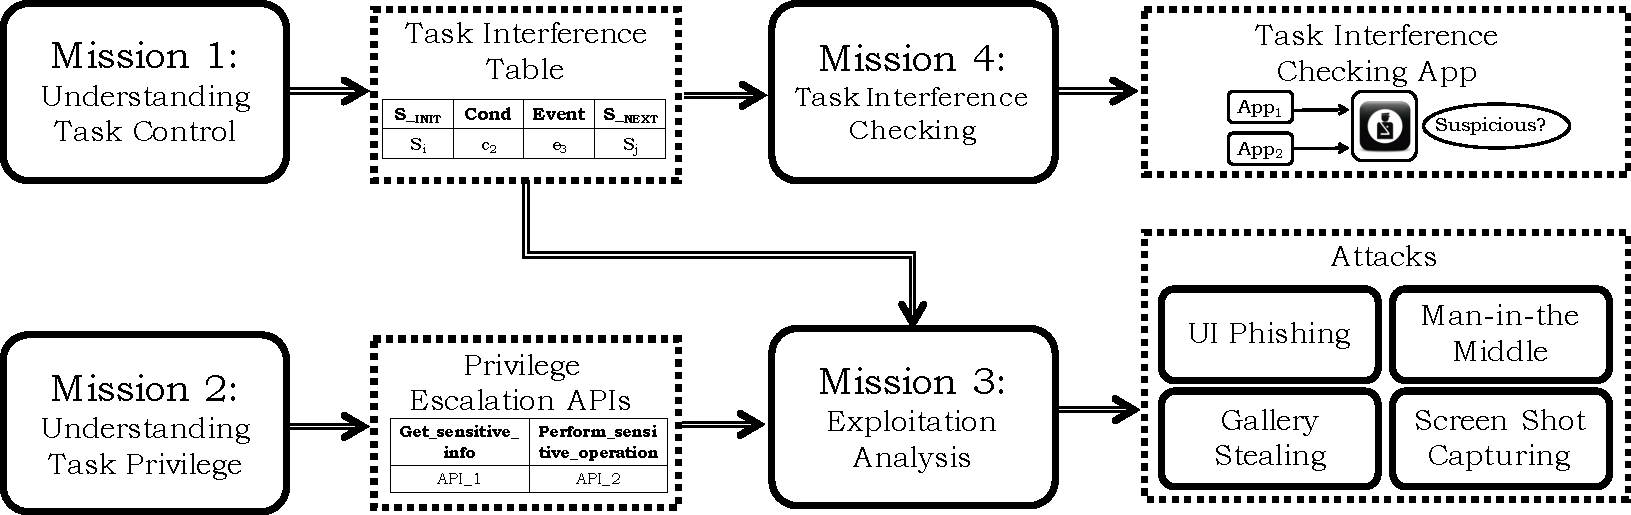
\includegraphics[width=1\linewidth]{overall.pdf}
        \caption{Approach Overview}
        \label{fig:arch}
\end{figure*}
\subsection{Security Analysis of Android Task Structure}\label{sec:atmapproach}
In this subsection, we introduce our approach. We focus on two aspects of
the Android task mechanism. First, We analyze the conditions that
affect Android task control to identify different ways that can
include an app into a task. Second, we explore the privilege an app
can get when it is included into a task. These are two necessary
components to identify new attacks.


\subsubsection{Understanding Android Task Control Conditions}

We explore the conditions and actions of Android task control through
dynamic testing.  To do this, we examine the Android
documentation~\cite{taskdoc} to create test cases to drive the
exploration. Our goal is to check the influence of the flags
introduced in Section~\ref{sec:preliminaries} on the task mechanism.

{\noindent \bf Testing Methodology.} We implemented the two template
apps introduced in Section~\ref{sec:threatandapproach}, AppB and AppM, as the
inputs to drive the testing process.  For each combination of the
task-control-related flags, such as {\em launchMode} and {\em
  taskAffinity}, we set the corresponding value in app templates,
create a pair of AppB and AppM, and test them with different sequences
of launching events, e.g., using the Android Launcher to start AppB
(denoted as Launcher$\rightarrow$AppB) or using AppB to launch AppM
(denoted as AppB$\rightarrow$AppM). During our test, AppB's {\em
  taskAffinity} is set to ``TaskB''.  We only test the conditions
where AppM's {\em allowTaskReparenting} is set to ``true'', as a
``false'' value in this flag will not result in task interference.

The results are summarized in Table~\ref{tbl:taskinterference}.  We
are interested in cases with potential task interference, i.e., AppM
ends up running as part of TaskB.  We mark the cases for task
interference, i.e., AppM running as part of TaskB, with an asterisk
``*''. The cases without an asterisk attached are considered to be
safe. We list four identified dangerous cases below.

\begin{itemize}
  \item {\bf Case 2}. Under the conditions of this case, AppM is
    launched first by the Android Launcher, followed by AppB. Only
    AppM runs at the foreground, while AppB cannot be executed.

    In this case, AppM blocks AppB from execution, which is a case
    of denial-of-use to AppB.
  \item {\bf Case 4}. Under the conditions of this case, AppM is
    launched by the Android Launcher, followed by AppB. AppB runs in
    the foreground, and AppM runs in the background, both in TaskB.
  \item {\bf Case 9}. Under the conditions of this case, the Android
    Launcher starts AppM. AppM then starts AppB. AppB runs in
    the foreground, and AppM runs in the background, both in TaskB.
  \item {\bf Case 10}. Under the conditions of this case, the Android
    Launcher starts AppB. AppB then starts AppM. AppM runs in
    the foreground, and AppB runs in the background, both in TaskB.
\end{itemize}

Whether two Apps are in the same task can be determined by
viewing the \emph{Recents} screen which renders all processes that
were opened since last clearance\cite{recents}. \emph{Recents} screen
is rendered when a user presses the \emph{Recents} button which is
located at the third from left to right at the button bar followed by
\emph{Back} and \emph{Home} buttons. If two Apps are in the same task,
\emph{Recents} screen will only show one process other than two when
they do not reside in the same task. Note that according to our
experiment, flags such as \texttt{FLAG\_ACTIVITY\_CLEAR\_TOP} and
\texttt{FLAG\_ACTIVITY\_REORDER\_TO\_FRONT} do not pose a difference
than the \texttt{SIGLE\_TOP} in our case. Therefore, we only include
the \texttt{SINGLE\_TOP} flag in our Table~\ref{tbl:taskinterference}.

\begin{table*}
\scriptsize
\centering
\caption{Task Interference Table}
  \floatfoot{We assume AppB is running with the
  task ``TaskB.'' In the events, the operation A$\rightarrow$B stands
  for A launches B. In the resulting state's status, F stands for
  execution in foreground; B stands for execution in background; X
  stands for not-running.}
\label{tbl:taskinterference}
\resizebox{\columnwidth}{!}{%
\begin{tabular}{|l|c|c|c|c|c|c|c|c|}
\hline
\textbf{Case \#}                              &
\multicolumn{4}{c|}{\textbf{Initial Conditions}}         &
\textbf{Events} &
\multicolumn{3}{c|}{\textbf{Resulting State}}           \\
\cline{2-5} \cline{7-9}
& AppB & \multicolumn{3}{c|}{AppM} & &
AppB &  \multicolumn{2}{c|}{AppM} \\
\cline{2-5} \cline{7-9}
& LaunchMode & LaunchMode & TaskAffinity & Reparenting &  & Status &
Status & Task\\
\hline \hline
1  &  standard or & standard or & TaskB  & True
   & Launcher$\rightarrow$AppB; Launcher$\rightarrow$AppM    & F & X & - \\

   &  singleTop or & singleTop or &        &
   &                                   &   &   &  \\

   & flag(SINGLE\_TOP) & flag(SINGLE\_TOP) & &
   &                                   &   &   &  \\
\hline
2  &  standard or & standard or & TaskB  & True
   & Launcher$\rightarrow$AppM; Launcher$\rightarrow$AppB    & X & F & TaskB \\

*  &  singleTop or & singleTop or &        &
   &                                   &   &   &  \\

   & flag(SINGLE\_TOP) & flag(SINGLE\_TOP) & &
   &                                   &   &   &  \\
\hline
3  &  singleTask or & standard or & TaskB  & True
   & Launcher$\rightarrow$AppB; Launcher$\rightarrow$AppM    & F & X & - \\

   & flag(NEW\_TASK) & singleTop or & &
   &                                   &   &   &  \\

   &                 & flag(SINGLE\_TOP) & &
   &                                   &   &   &  \\

\hline
4  &  singleTask or & standard or & TaskB  & True
   & Launcher$\rightarrow$AppM; Launcher$\rightarrow$AppB    & F & B & TaskB \\

*  & flag(NEW\_TASK) & singleTop or & &
   &                                   &   &   &  \\

   &                 & flag(SINGLE\_TOP) & &
   &                                   &   &   &  \\

\hline
5  &  singleTask or & singleTask or & TaskB  & True
   & Launcher$\rightarrow$AppB; Launcher$\rightarrow$ AppM     & B & F & TaskM \\

   & flag(NEW\_TASK) & flag(NEW\_TASK) & &
   &                                   &   &   &  \\
\hline

6  &  singleTask or & singleTask or & TaskB  & True
   & Launcher$\rightarrow$ AppM ; Launcher$\rightarrow$AppB    & F & B & TaskM \\

   & flag(NEW\_TASK) & flag(NEW\_TASK) & &
   &                                   &   &   &  \\
\hline

7  &  singleInstance or & any or & TaskB  & True
   & Launcher$\rightarrow$AppB; Launcher$\rightarrow$AppM    & F & X & - \\
\hline

8  &  singleInstance or & any or & TaskB  & True
   & Launcher$\rightarrow$AppM; Launcher$\rightarrow$AppB    & F & B & TaskM \\
\hline

9  &  standard or & standard or & TaskB  & True
   & Launcher$\rightarrow$AppM; AppM$\rightarrow$AppB  & F & B & TaskB \\

*   &  singleTop or & singleTop or &        &
   &                                   &   &   &  \\

   & flag(SINGLE\_TOP) & flag(SINGLE\_TOP) & &
   &                                   &   &   &  \\
\hline

10  &  standard or & standard or & TaskB  & True
   & Launcher$\rightarrow$AppB; AppB$\rightarrow$AppM  & B & F & TaskB \\

*   &  singleTop or & singleTop or &        &
   &                                   &   &   &  \\

   & flag(SINGLE\_TOP) & flag(SINGLE\_TOP) & &
   &                                   &   &   &  \\
\hline
\end{tabular}
}
\end{table*}

\subsubsection{Understanding Privilege Obtained in the Same Task}
\label{sec:priv}

From the results in Table~\ref{tbl:taskinterference}, we can see that
AppM has several ways to be included into the task of AppB, often
without involving actions from other apps or the system. Next, we
explore the privilege obtained through the Task mechanism, including
privilege for retrieving other apps' information and privilege for
changing other apps' states. Therefore, if the privilege given to apps
in the same task allows them to carry out dangerous actions, it can be
potentially misused by the malicious app.

\textbf{Retrieving Information of Other Apps}

\noindent

Figuring out the execution state of a victim app, such as whether it
is running and which activity is in foreground, is often used as the
first step in several attacks, such as UI
hijacking~\cite{UIstateinference}. Therefore, Android by default disallows one app
from directly querying another app's runtime information from through
the Android sandbox policy.

In older versions of Android, there were APIs allowing inter-app
runtime information checking.
For devices that are prior to \textit{Android Lollipop
  (v5.0)}, directly calling the API
\texttt{getRunningTasks(int maxNum)} will return the information of as
many as \texttt{maxNum} running activities~\cite{getrunningtask}.
However, this function is deprecated after \textit{Lollipop} since allowing third-party apps to invoke the function
directly will cause information leakage in important apps.

For devices prior to \textit{Android MarshMallow (v6.0)}, directly
calling \\
\texttt{getRunningAppProcesses()} returns a list of
application processes that are running on the
device~\cite{getrunningtask}. This function returns a
\textit{RunningAppProcessInfo} object, which includes a member
variable called \textit{importance} that represents the importance
level that the system places on the
process~\cite{processimportance}. It has one of these values:
\texttt{IMPORTANCE\_FOREGROUND}, \texttt{IMPORTANCE\_VISIBLE},
\texttt{IMPORTANCE\_SERVICE}, \texttt{IMPORTANCE\_BACKGROUND} and
\texttt{IMPORTANCE\_EMPTY}. If \textit{importance} is
\texttt{IMPORTANCE\_FOREGROUND}, the corresponding process is running
in the foreground. This method, however, cannot accurately point out
which activity running in the foreground since it operates on a
process level and accesses only the package name.  This method is also
no longer supported for \textit{MarshMallow} devices with API level 23
unless the third-party app who is making a call to this function has
the same process ID as the target process.


\paragraph*{Getting App Running Information in a Task.}
Although the Android API \\
\texttt{getRunningTasks()} is deprecated for
direct usage, we have found that it still works if the calling app and
the target app are in the same task.  The official documentation of
\texttt{getRunningTasks()} does not explicitly point it out but only
states that if it is called, this function only returns a small
subsets of information, e.g., the information of the caller's own task
and home task which is considered to be not
sensitive~\cite{getrunningtask}.


\textbf{Changing States of Other Apps}

\noindent

\paragraph*{UI Injection.}
Ideally, if an app is running in the foreground, other apps isolated
from this app should not perform sensitive operations on it. Chen {\em et
al.}~\cite{UIstateinference} show two UI-injection methods that do not
require any permissions: (1) starting an \texttt{Activity} by setting
\texttt{lauchMode=singleInstance}. This is also how most system apps,
such as the alarm app, pop up a window on the top of another
app~\cite{androidlaunchmode}; (2) starting an \texttt{Activity} from
the Android broadcast receiver~\cite{androidbroadcastreceiver}.

In our analysis, we find that if two apps are in the same task, the
UI-injection attack becomes easier.  The attacker can simply call the
function \texttt{startActivity()} to achieve the same effect. Through
understanding the Android SDK source code, \texttt{startActivity()}
invokes \texttt{startActivityForResult()} with
\texttt{requestCode=-1}. Later \\
\texttt{startActivityForResult()}
invokes \texttt{execStartActivity()} in the Instrumentation class, a
base class for implementing application instrumentation
code~\cite{Instrumentation}. \\
 \texttt{execStartActivity()} then checks
the base package of the calling activity by invoking
\texttt{getBasePackageName()}. If the base package of calling activity
matches with that of target activity, the Android system launches the
target activity.

\paragraph*{Terminating UI.}
Android does not allow a third-party app to terminate a running app
unless they are in the same process. Although an app is not in the
foreground, the Android system still allows any third-party apps to
make calls to
\texttt{killBackgroundProcesses()}~\cite{killBackgroundProcesses} to
terminate any specific background app. There is no direct way to
terminate a foreground-running activity.

Unlike \texttt{startActivity()}, even if two apps are in the same
task, calling \texttt{finish()} or \texttt{finishActivity()} will not
terminate the foreground activity, but will terminate the activity
that makes the call. However, we found that as long as two apps are in
the same task, calling the API \texttt{finishAndRemoveTask()} results
in terminating the whole Task regardless of whether an activity is
running in the foreground~\cite{finishAndRemoveTask} or not.
This provides the malicious app an interface to terminate other apps which are within the same task as it.

\subsection{Information Stealing Attacks}\label{sec:infoattack}
Based on analysis from Section~\ref{sec:atmapproach}, we develop
four proof-of-concept attacks: \textsl{UI Phishing},
\textsl{Activity-in-the-middle Attack}, \textsl{Gallery Stealing}, and
\textsl{Screen Shot Capture}. These four attacks demonstrate the
severity of the security problems we identified. In this subsection, the
attacks are illustrated using two most popular social apps, Instagram
and Facebook. Except Gallery Stealing, which requires
\texttt{READ\_EXTERNAL\_STORAGE}, all other three attacks only require
the \texttt{INTERNET} permission~(in order to send out the information
stolen).

\subsubsection{UI Phishing}
UI Phishing is a popular type of attacks to spoof users.  The
difficulty of phishing attack is to decide the timing when the
spoofing interface should be prompted, in order to prevent the victim
from noticing it.  Ren {\em et al.}~\cite{TaskHijacking} introduced
``Back Hijacking'', which directs users to a spoofed bank
\textit{LoginActivity}. The key difference is that the attack method
identified in our approach {\em actively} interact with the victim app
using the privilege obtained through the approaches we discussed in
Section~\ref{sec:priv}.

Our proof-of-concept UI Phishing attack is implemented against
the scenario when a user logs in to Instagram using his/her Facebook
account.  In order to ease understanding the phishing attack against
this scenario, we brief the Facebook SSO service.  According to the
Facebook Android developer documentation~\cite{FacebookLoginWays},
Facebook SDK takes three ways for apps who require Facebook Login as
part of functionality:

\begin{itemize}
\item {\bf Native App Login.}
If the Android device already has the Facebook app installed, pressing
the Facebook login button directly opens the Facebook app where user
can log in his/her Facebook account and grants permission to the
third-party app to access his/her Facebook personal information.

\item \textbf{Chrome Custom Tab Login. }
If the Android device does not have the Facebook app installed, a
third-party app can ask the Chrome browser to open Facebook login page
by registering a scheme in the \texttt{Manifest} with the format
\texttt{fb+facebook\_app\_id}.

\item {\bf WebView Login.}
Finally if neither the Android device has Facebook app installed, nor
does the third-party app register for Chrome Custom Tab Login, an
embedded WebView will be launched dynamically rendering the content of
Facebook login page.
\end{itemize}

Our attack works when a user presses the ``Log in with Facebook''
button in Instagram. We assume that a user already has Facebook App
installed in the device. Instagram includes Facebook Login as a part
of its functionality. It does not register for Chrome Custom Tab
Login. In other words, after pressing the ``Log in with Facebook''
button in Instagram, it will launch Facebook App directly. The package
name of Facebook app is \texttt{"com.facebook.katana"}, the package
name of self-build WebView is \texttt{"com.android.webview"} and the
package name of Instagram is \\
\texttt{"com.instagram.android"}.  Shown
in Figure~\ref{fig:uiphishing}, it works in the following steps.

\begin{figure*}[t!]
        \centering
        \begin{subfigure}[t]{0.5\textwidth}
                \centering
                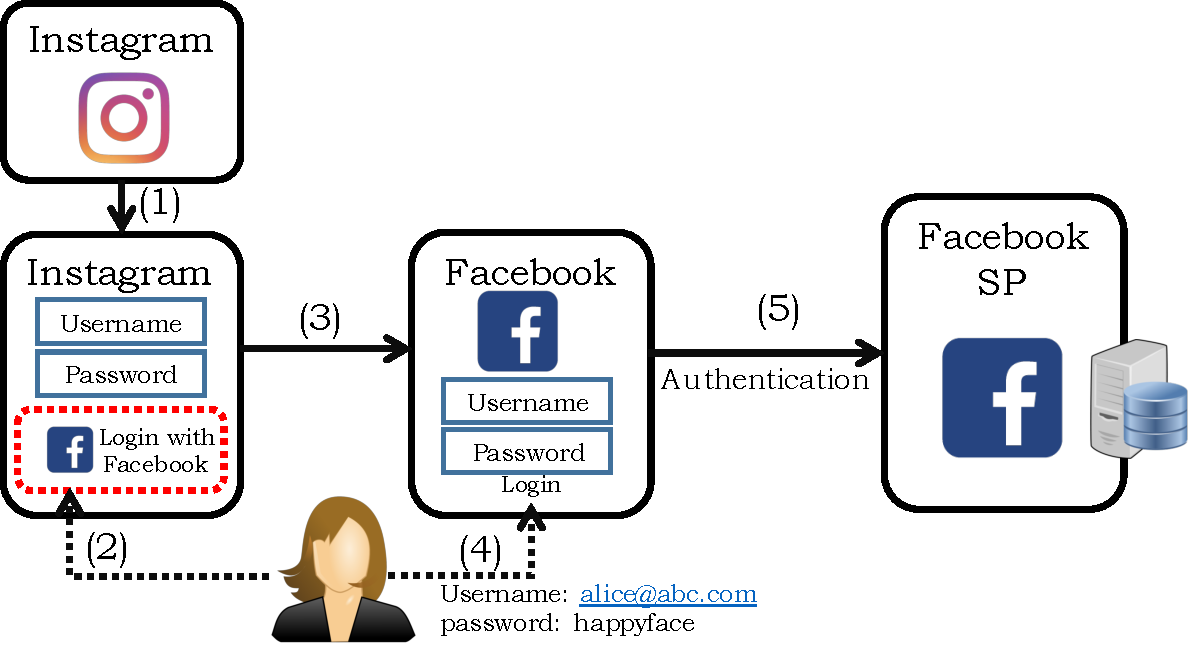
\includegraphics[width=\linewidth]{attack-phishing-0.pdf}
                \caption{Single-Sign-On Architecture}
          \end{subfigure}%
          %\quad
        \begin{subfigure}[t]{0.5\textwidth}
                \centering
                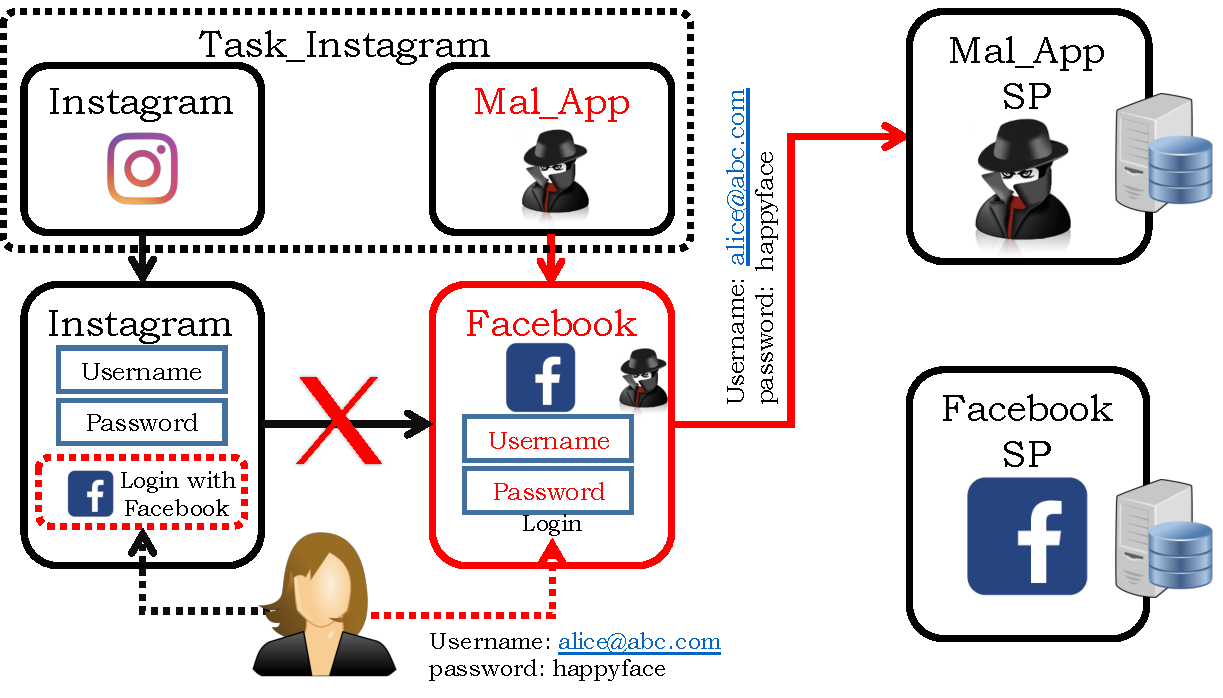
\includegraphics[width=\linewidth]{attack-phishing-1.pdf}
                \caption{UI Phishing Attack}
        \end{subfigure}
        \caption{UI Phishing}
         \floatfoot{(a) When the user selects
          ''login with Facebook'' in Instagram, Instagram will launch
          the Facebook app. After the user inputs username, password
          and finishes the authentication with the Facebook service
          provider, Instagram gets the permission to access the user's
          Facebook resources. (b) The malicious app Mal\_App declares
          same taskAffinity as Instagram. Mal\_App creates a
          background thread and monitors the running states of
          Instagram. When the user selects Facebook login button and
          Instagram launches the Facebook activity, Mal\_App will
          override Facebook with a fake login UI. The
          username/password input by the user will be sent to
          Mal\_App's service provider.}
           \label{fig:uiphishing}
\end{figure*}



\textbf{(1)} Attacking app declares the same task as Instagram. This step
can be achieved by setting the attributes of \textit{taskAffinity} and
\textit{allowTaskReparenting} as follows.
\begin{lstlisting}[language=XML]
 <activity
            android:name=".UIPhishingActivity"
            android:allowTaskReparenting="true"
            android:taskAffinity="com.instagram.android">
\end{lstlisting}

\textbf{(2)} The launcher first launches the attacking app, which
launches Instagram immediately through invoking the task parent since
Instagram is the parent of the current task. Before Instagram's
\texttt{setContentView(R.layout.main)} function can be called, the
attacking app launches Launcher (Home), meaning that Instagram cannot
be displayed in order to achieve the stealthiness. The process can be completed in a fairly short time and will not be noticed by the victim with bare eyes. After that, our attacking app waits for victim to launch Instagram herself.


\textbf{(3)} The attacking app then creates a background thread which
runs in a cycle of, we devise, every 100 milliseconds. In the
meantime, it checks whether there is a change in the foreground
package name, i.e., in our case, the package name changes from \\
\texttt{"com.android.webview"} to \texttt{"com.facebook.katana"}. This
can be achieved by simply making API call to
\texttt{getRunningTasks()}. Once the foreground package has been
changed to Facebook, our attack pops up our counterfeit Facebook
\textit{LoginActivity} overriding the real one. The spoofed UI
collects the user's login information and send it to adversary's
back-end server.

\subsubsection{Activity-in-the-middle Attack}
The Facebook SSO process is based on OAuth
2.0~\cite{OAuthDemystified}. The main steps of this mechanism are: (1)
When the user opens the relying party (RP) app, in our case,
Instagram, it passes its \texttt{Facebook\_app\_id} and directed URL
to the Android System.  (2) The Android system then redirects user to
the Service Provider (SP), in our case, Facebook, and passes it the
\texttt{Facebook\_app\_id}.  (3) If the user requests to grant the
permission to the RP, SP will issue an access token to the Android
system.  (4) The Android system passes the access token to RP, by
which RP is able to access the user's protected resource on SP.

Facebook has two types of access tokens, short-term and
long-term~\cite{fbaccesstoken}. Short-term access token lasts several
hours and long-term lasts for 60 days. Unless specifically required,
Facebook usually issues short-term access token. RPs use graph API
provided by Facebook to retrieve protected resources hosted on
Facebook server~\cite{graphapi}. Graph API is an HTTP-based API, which
is implemented as the following URL:
 \begin{lstlisting}
 https://graph.facebook.com/me?fields=xxx&access_token=xxx
 \end{lstlisting}

In other words, any party who has the access token can access the
user's protected resources hosted on Facebook servers.

In Android, redirecting to the Facebook app is done by intent
transition based on \texttt{startActivityForResult()} and
\texttt{onActivityResult()}.  We implement an MITM attacking app whose
model runs in the following steps, shown in Figure~\ref{fig:mitm}.

\textbf{(1)} It follows the first three steps in the UI Phishing
attack model.

\textbf{(2)} Instead of popping up a phishing login
page like UI Phishing, the MITM attack pops up a transparent activity,
which blocks the traffic that is supposed to be relayed to Facebook
server from user's device system and passes our own traffic to
Facebook. This step can be easily realized by creating an invisible
Facebook Login Button and sending a button pressed event itself by
invoking \texttt{mFacebookLoginBtn.performClick()}.

\textbf{(3)} After the user grants the permission, which he/she
intends for Instagram, the MITM app retrieves the access token. Since
Instagram runs in the background, once the foreground finishes,
Instagram will be invoked.


\textbf{(4)} To finalize the process, the adversary needs to verify
\texttt{APP\_ID} and \emph{App Secret} with Facebook. An adversary can
either register its attacking app in Facebook Developer Website and
use its own \texttt{APP\_ID} and \emph{App Secret} or steal other RP
apps' ID and Secret. Facebook RP Apps will post an HTTP message when
user system launches native Facebook App.

\begin{figure*}[t]
        \centering
        \begin{subfigure}[t]{0.5\textwidth}
                \centering
                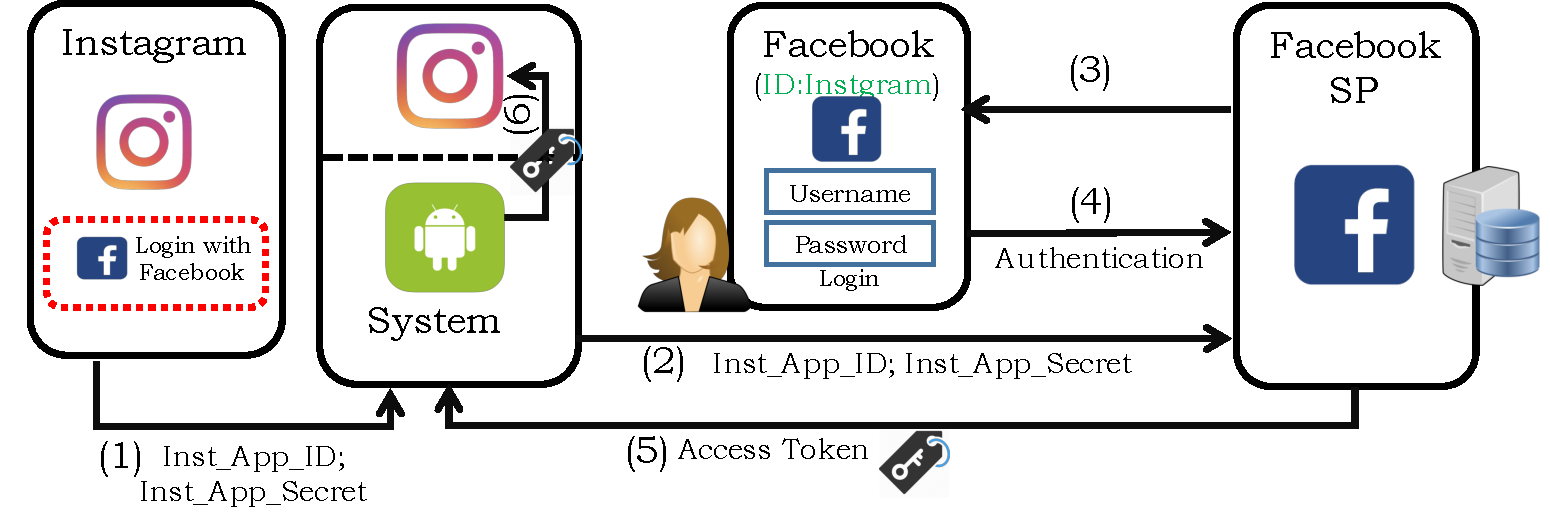
\includegraphics[width=\linewidth]{attack-mim-0.pdf}
                \caption{Single-Sign-On Permission Granting Architecture}
          \end{subfigure}%
          %\quad
       \begin{subfigure}[t]{0.5\textwidth}
                \centering
                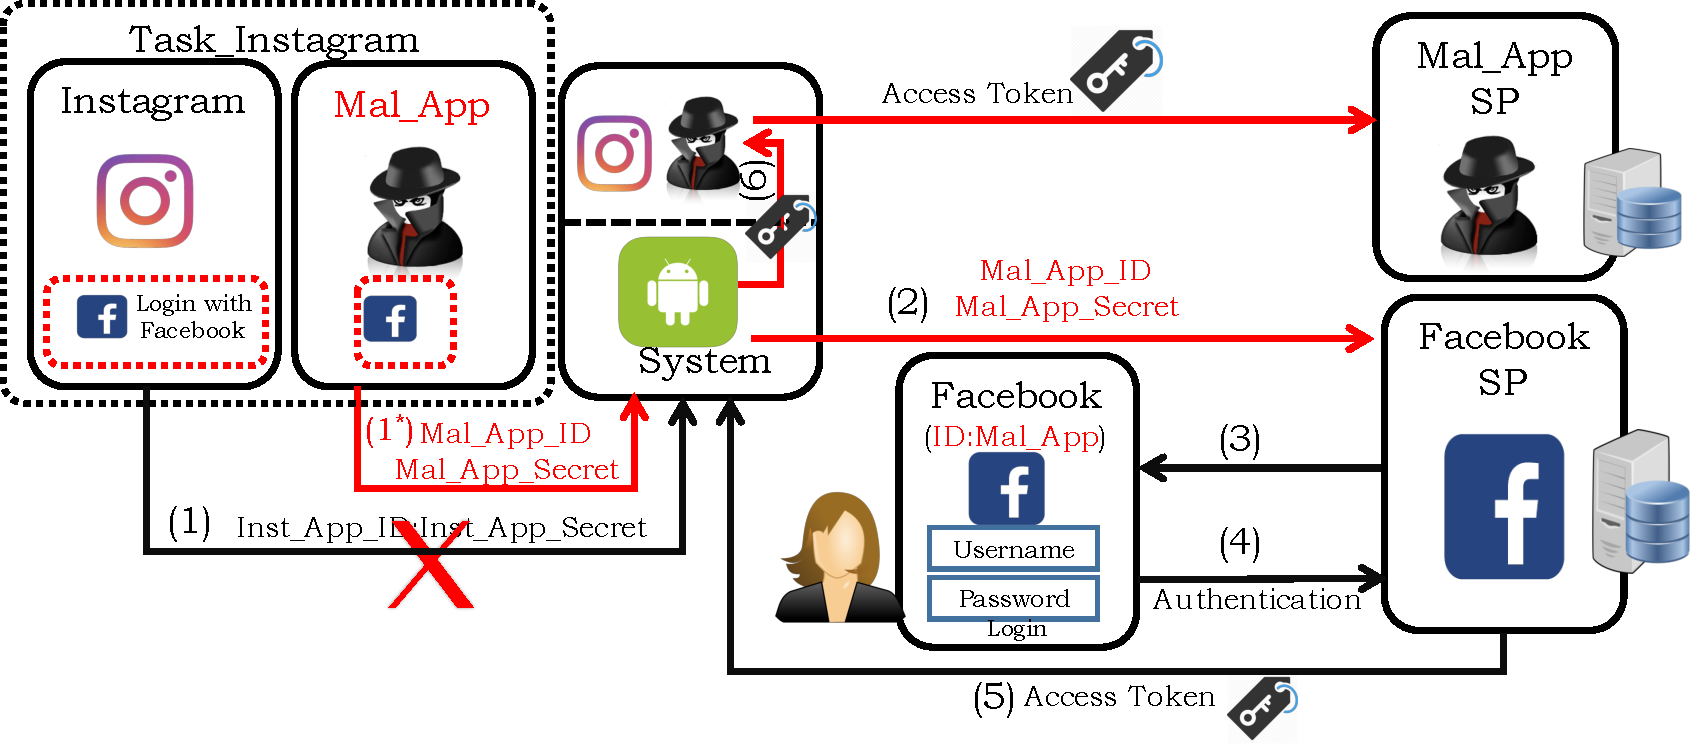
\includegraphics[width=\linewidth]{attack-mim-1.pdf}
                \caption{Activity-in-the-Middle Attack}
        \end{subfigure}
        \caption{Activity-in-the Middle Attack on SSO}
        \floatfoot{(a) When a
          user wants to login with Facebook in the Instagram,
          Instagram sends system its application ID with application
          secret, Inst\_App\_ID and Inst\_App\_Secret. Android system
          forwards request with Inst\_App\_ID and Inst\_App\_Secret to
          Facebook service provider and retrieves Facebook Login
          Activity bound with Inst\_App\_ID. The user inputs her/his
          username/password for authentication. Facebook service
          provider returns the access token to Android system if the
          authentication passed. Android system sends the access token
        to Instagram according to the application ID that system
        received. (b) The malicious app Mal\_App overrides the
        ownership of the Instagram task in the same way as
        UI-phishing. It monitors the Instagram running status and
        sends system its Facebook login request (including Mal\_App\_ID and
        Mal\_App\_Secret) before the Instagram's request arrives
        Android system. Android system sends Mal\_App's request to
        Facebook service provider and
        drops the same login request arrived later. Facebook return
        Login Activity bound with Mal\_App\_ID. The user inputs her/his
          username/password for authentication. Facebook service
          provider returns the access token to Android system if the
          authentication passed. Android system sends the access token
        to  Mal\_App according to the application ID that system
        received.}
        \vspace{-0.2cm}
           \label{fig:mitm}
\end{figure*}

\subsubsection{Gallery Stealing}
Starting from Android 6.0 (API level 23), in order to access gallery,
an app has to request for \texttt{READ\_EXTERNAL\_STORAGE} permission
at runtime rather than at the installation time, which is classified
as one of the dangerous permissions~\cite{permissionruntime}. This
mechanism provides more secure and flexible protection to user's photo
gallery.  However, this new security mechanism can be bypassed by
exploits to the Android task mechanism, as shown in this subsection.

\noindent\textbf{Timing.} 
For Android devices before \textit{marshmallow} (API level lower than
23), permissions are requested at the time when an app is being
installed. Apps with suspicious permissions will easily trigger the
user's attention and likely be denied access. However, with the new
requesting-permissions-at-run-time mechanism, our attacking app can
avoid requesting permission when being installed since it is requested
at the run time. To figure out the suitable timing, it continuously
monitors Instagram.  Once the victim clicks the ``Camera'' button on
Instagram which allows Instagram to access the gallery and camera, our
attacking app instantly kills Instagram and pops up our requesting
dialog for access photos in gallery. User mistakenly believes that
he/she is granting the permission to Instagram. After the permission
is granted, our attacking app retrieves all the photos from user's
gallery and send them to the back-end server. In order to be
stealthier, the attacking app pops up a dialog shows ``System
encounters errors'' and finally kills itself.

\noindent\textbf{Permission Dialog.}
Even though timing improves the naturalness of the attack, Android
permission dialog shows the name of the app in bold who makes the
request. We propose two ways to circumvent this
problem.
\\\textbf{(1)} By employing the idea of social engineering, the attacker can name the attacking app 
using a name similar to the target app. In our case,
e.g., ``Instgram'' or ``Instagam''. However, naming the app in this way
can hardly pass the review of Google Play. Even if it does, careful
users may still notice the difference. Therefore, in our attack, we do not
use this method.

\noindent \textbf{(2)} Employing the tapjacking. The idea of tapjacking
is putting message the attacker wishes to display on the top of the
real system message by setting a window layout flag
\texttt{TYPE\_SYSTEM\_OVERLAY}. Android realizes the potential threat
and adopts the mechanism
\texttt{MotionEvent.FLAG\_WINDOW\_IS\_OBSCURED} which alerts the real
dialog is being overlaid\cite{flagwindowobscured}. Unfortunately,
Bana\'s\cite{TapjackingIwo} found that \\
\texttt{MotionEvent.FLAG\_WINDOW\_IS\_OBSCURED} is not triggered if
the covered text does not cover the touch points, which are the
buttons in the dialog. Android does not give a patch to the issue.
Instead, it adopts an intent transition scheme to notify the user that
the content is being overlaid starting from Android 6.0 (API level
23). We managed to circumvent the issue by implementing our main
attacking app with \texttt{targetSdkVersion=23}, and in the target app
we tricked the user to install a helper package, which is an
activityless service.  Only app which has the
\texttt{targetSdkVersion=22} and has the overlaying functionality
implemented. It seems tricking users to install additional package is
not applicable, but it is in fact a very common situation for many
apps such as those who require Android SQLite Manager.

The basic steps of the attack model are listed as
follows.

\textbf{(1)} The attack follows the first three steps of UI Phishing
attack.

\textbf{(2)} Once a user presses the camera button of Instagram as
shown in Figure~\ref{fig:gallery}(a), the foreground \texttt{Activity}
will change to
\texttt{"com.instagram.android.creation.activity.\-MediaCaptureActivity"}. Therefore,
Instead of detecting whether the foreground package has changed to
another app, we zoom in the design to focus on changing of the
foreground \texttt{Activity}.

\textbf{(3)} Instead of popping up a counterfeit
page like UI Phishing does, it pops up an \texttt{Activity} which
immediately asks a user for \texttt{READ\_EXTERNAL\_STORAGE} so that
the user thinks he/she is granting the permission to Instagram.

\textbf{(4)} Once the attack app gets the permission, it traverses all the pictures and transmits the image buffers to server.

\textbf{(5)} To achieve better stealthiness, we introduce the
Tapjacking to assist our attack. Its basic idea is to cover the real
texts with some fake texts. Then we are able to change the text of the
permission dialog to ``Allow Instagram to access ...?'' instead of the
real text which is ``Allow GalleryStealing to access ...?'', which is
shown in Figure~\ref{fig:gallery}(b). Once user grants the
permission, the app quickly sends all images as buffer to the server.
Meanwhile, it fools the user by showing a ``system warning dialog''
telling the user that the system encounters an error (shown in
Figure~\ref{fig:gallery}(c)).


\begin{figure*}[t]
        \centering
        \begin{subfigure}[b]{0.325\textwidth}
                \centering
               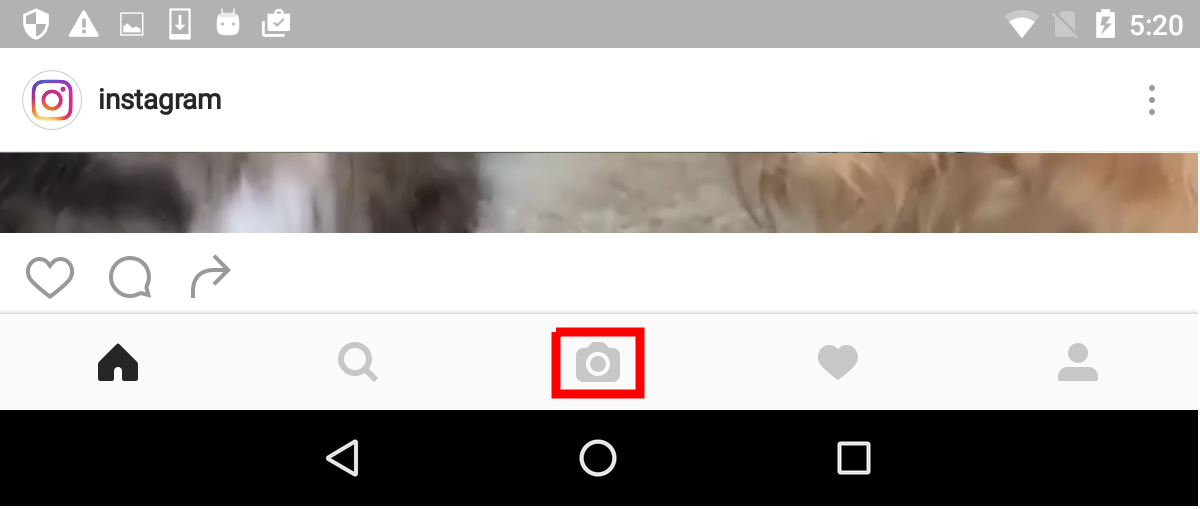
\includegraphics[width=\linewidth]{4-1}
                \caption{}
        \end{subfigure}
        \begin{subfigure}[b]{0.3\textwidth}
                \centering
          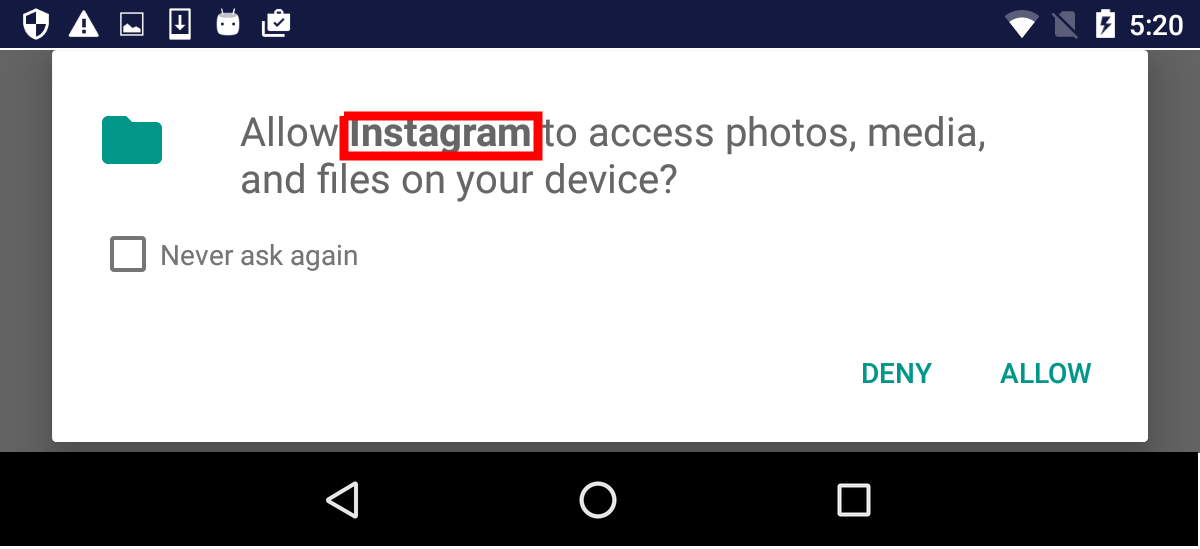
\includegraphics[width=\linewidth]{4-2}
                \caption{}
        \end{subfigure}
        \begin{subfigure}[b]{0.35\textwidth}
                \centering
          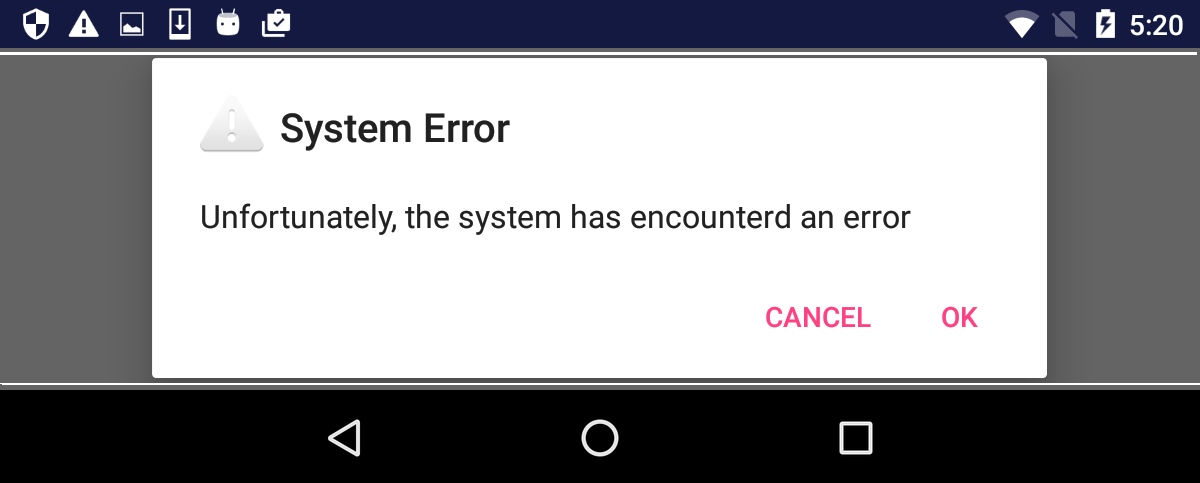
\includegraphics[width=\linewidth]{4-3}
                \caption{}
        \end{subfigure}
         \caption{Gallery Stealing Attack}
         \floatfoot{First the user clicks the camera button highlighted in the first picture. Then the attacking app	kills the real Instagram and pops up its \texttt{Activity} asking for user permission, the text of permission dialog is overlaid by the fake text as shown in the second picture. Once user grants the permission, the app quickly sends all images as buffer to the server, meanwhile, it fools the user by showing a ``system'' warning dialog telling the user the system encounter an error.}
         \label{fig:gallery}
\end{figure*}

\subsubsection{Screen Shot Capturing}
With the ability of knowing which \texttt{Activity} is currently
running in the foreground, we implement this screen shot capturing
attack which starts taking screen shots while a user is entering
username and password in the Facebook \texttt{LoginActivity} which is
\texttt{com.facebook.katana.LoginActivity} in full. For password
typing, every time a character is entered, the character will be shown
for a short time before it turns into a star sign. Therefore, taking
screen shot every 0.1 second should capture everything a user types in
password box.


With respect to taking a screen shot programmatically, we summarize
four possible ways:
\begin{itemize}
\item {\bf Using READ\_FRAME\_BUFFER Permission.}  Declaring
  \texttt{READ\_FRAME\_BUFFER} permission in the \texttt{Manifest}
  allows an application to take screen shots by making calls to
  \texttt{ISurfaceComposer} \cite{framebuffer}. However, this
  permission is not available to third-party application unless it has
  the same signature as the system does.

\item {\bf Using fb*.} Some Linux systems store frame buffers in
  \texttt{/dev/graphics/fb*} or \texttt{/dev/fb*}. \texttt{fb0}
  represents the first frame buffer, \texttt{fb1} represents the
  second frame buffer and so on.  Using native C/C++ code to get
  access to these files and copy the buffer as a \texttt{GGLSurface}
  structure is theoretically possible. But there are two unsolvable
  obstacles of this method:
  \begin{itemize}
  \item This method requires root permission.
  \item It is likely that \texttt{fb*} does not even exist.
  \end{itemize}

\item {\bf Using Backup Channel over USB.}  Android system uses
  Android Debug Bridge (ADB) to listen to the debugging connections
  over USB~\cite{adb}. ADB has slightly more privileges than normal
  apps. Bai {\em et al.}~\cite{DBLP:conf/iceccs/BaiSWYLDG15} manage to
  exploit Backup Channel through ADB to steal access tokens from other
  apps. Combining ADB with Dalvik Debug Monitor Server (DDMS) tool
  enables an app to get the screen shot from the device without any
  permission~\cite{ddms}.

\item {\bf Using MediaProjection.}  For devices beginning in Android
  5.0 (API level 21), a class called \texttt{MediaProjection} was
  added to Android SDK which enables a third-party app to capture
  screen shot and record system audio\cite{mediaprojection}. While
  recording system audio requires \texttt{RECORD\_AUDIO} permission,
  capturing screen shots does not.
\end{itemize}

We employed the fourth method to capture screen shots. The basic steps
of the attack are listed as follows.\\ \textbf{(1)} It follows the
first three steps of UI Phishing. What's different is we devise this
attack to focus on Facebook App since we are hoping to steal user's
Facebook username and password. Hence, we declared this attack to
reside in the same task as Facebook.\\ \textbf{(2)} Once a user launches
the Facebook app, a transparent Activity is popped up start taking
screenshots. Although it does not require permission for taking screen
shots, it uses intent transition to let the user decide whether or not
an app can capture screen shots in a permission-like dialog. Again we
employ the tapjacking in Gallery Stealing attack to cover the text to
be ``Allow Facebook start accessing Internet?'' \\ \textbf{(3)} The
attack starts capturing screens by calling
\texttt{startActivityForResult()} which passes a screenshot as an
intent from which we can extract an object of \texttt{MediaProjection}
later, and finally use this \texttt{MediaProjection} object to pass
the image to an object of \texttt{ImageReader} through its member
function \texttt{createVirtualDisplay}. Since the screenshots are
taken in the \texttt{RGBA\_8888} format while bitmap takes
\texttt{ARGB\_8888}, we still need to do matrix transformations to
get the image.

\begin{figure*}[t]
        \centering
        \begin{subfigure}[b]{0.285\textwidth}
                \centering
               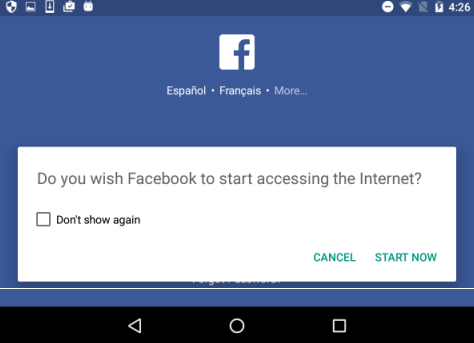
\includegraphics[width=\linewidth]{5-1}
                \caption{}
        \end{subfigure}
        \begin{subfigure}[b]{0.35\textwidth}
                \centering
          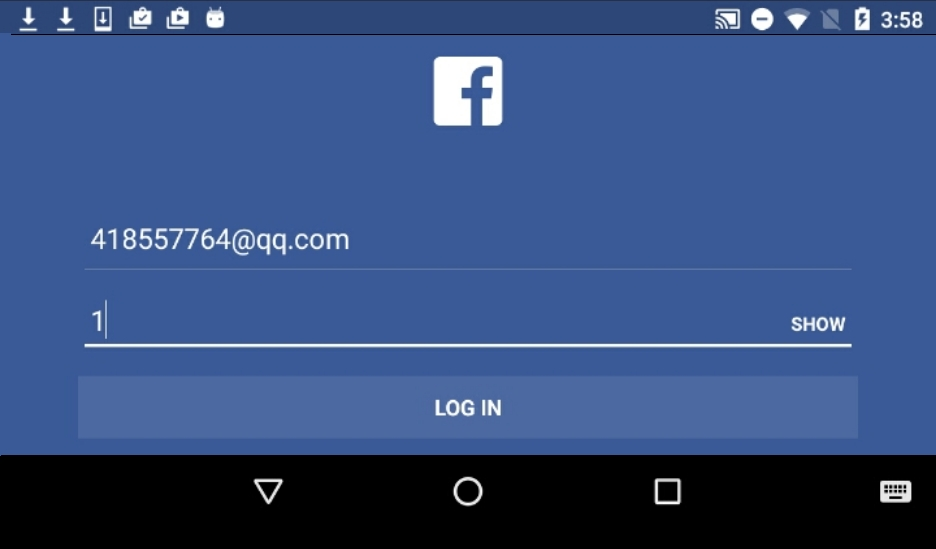
\includegraphics[width=\linewidth]{5-2}
                \caption{}
        \end{subfigure}
        \begin{subfigure}[b]{0.31\textwidth}
                \centering
          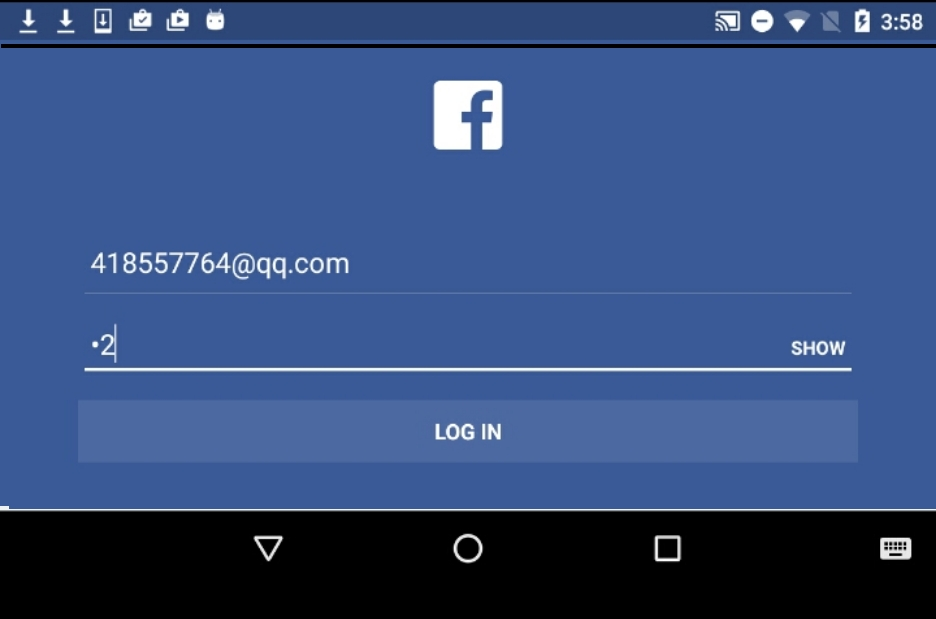
\includegraphics[width=\linewidth]{5-3}
                \caption{}
        \end{subfigure}
         \caption{Screenshot Capturing Attack}
         \floatfoot{First the user launches Facebook, then the attacking app launches a transparent \texttt{Activity} which quickly asks for taking screen shot, the notification dialog is again overlaid by fake text as shown in the first picture. Once the user clicks start now, the attacking app begins to take screen shots as well as sending the screen shots to back end server. (b) and (c) are two of the screen shots received by server which expose the password plaintext.}
         \vspace{-0.2cm}
         \label{fig:memory}
\end{figure*}

\subsection{Attack Performance}\label{sec:attackperf}

In order to study the feasibility of the four attacks, we implement them and evaluate them in
two aspects, \emph{time cost} and \emph{memory usage}.
% We check the average running time and the average virtual memory curves to illustrate the performance of our four proof-of-concept attacks.

\subsubsection{Time Cost}
We conduct 6 - 8 rounds of tests for every attack to calculate the average
running time cost. The testing results are summarized
in Table~\ref{tbl:time}. As shown in Table~\ref{tbl:time}, our attacks
are efficient since the time cost of most attacks is less than 8 seconds:
the UI Phishing attack costs 7.1 seconds, which includes user
interactions such as launching Instagram, entering username and
passwords; The Activity-in-the-middle attack costs time 5.8 seconds; and
the average time cost of the gallery-stealing attack is 4.6 seconds.

The Screenshot Capturing attack is an exception, taking 38.1
seconds. This attack uses much longer time because screenshots in
Android are passed in the format of RGBA, while we need to change to
ARGB in order to convert it to common format such as JPEG and PNG.
We perform the matrix transformation required for the conversion on
the mobile device. But since the process is undertaken in the background, it will
not trigger the suspicions of the user. In the real world attack, an
adversary can leave the job of matrices transformation to the server.

\begin{table}[h]
  \centering
\caption{Time Cost of Proof-of-Concept Attacks}
\label{tbl:time}
\begin{footnotesize}
\begin{tabular}{|c|c|}
  \hline
  \textbf{Attack} & \textbf{Time Cost (s)} \\
  \hline\hline
  UI Phishing & 7.1\\
  \hline
  Activity-in-the-Middle & 5.8\\
  \hline
  Gallery Stealing & 4.6 \\
  \hline
  Screenshot Capturing & 38.1\\
  \hline
\end{tabular}
\end{footnotesize}
\end{table}

\subsubsection{Memory Usage}

We conduct 3-round experiments for each attacks to get the memory
distractions of attacks and evaluate their average memory usage. The
testing results are illustrated in Figure~\ref{fig:memory}.  It shows
that the maximum memory usage of most attacks is less than $70MB$ except
Gallery Stealing attack, whose memory usage is around $100MB$. Our
testing results also disclose the memory usage distribution on
different period, in which the major memory usage of each attack is to
launch victim app (normal app), e.g., Instagram and Facebook. The
memory usage differences caused by stealthy behaviors/operations are
negligible.

\begin{figure}[h]
        \centering
        \begin{subfigure}[t]{0.5\textwidth}
                \centering
               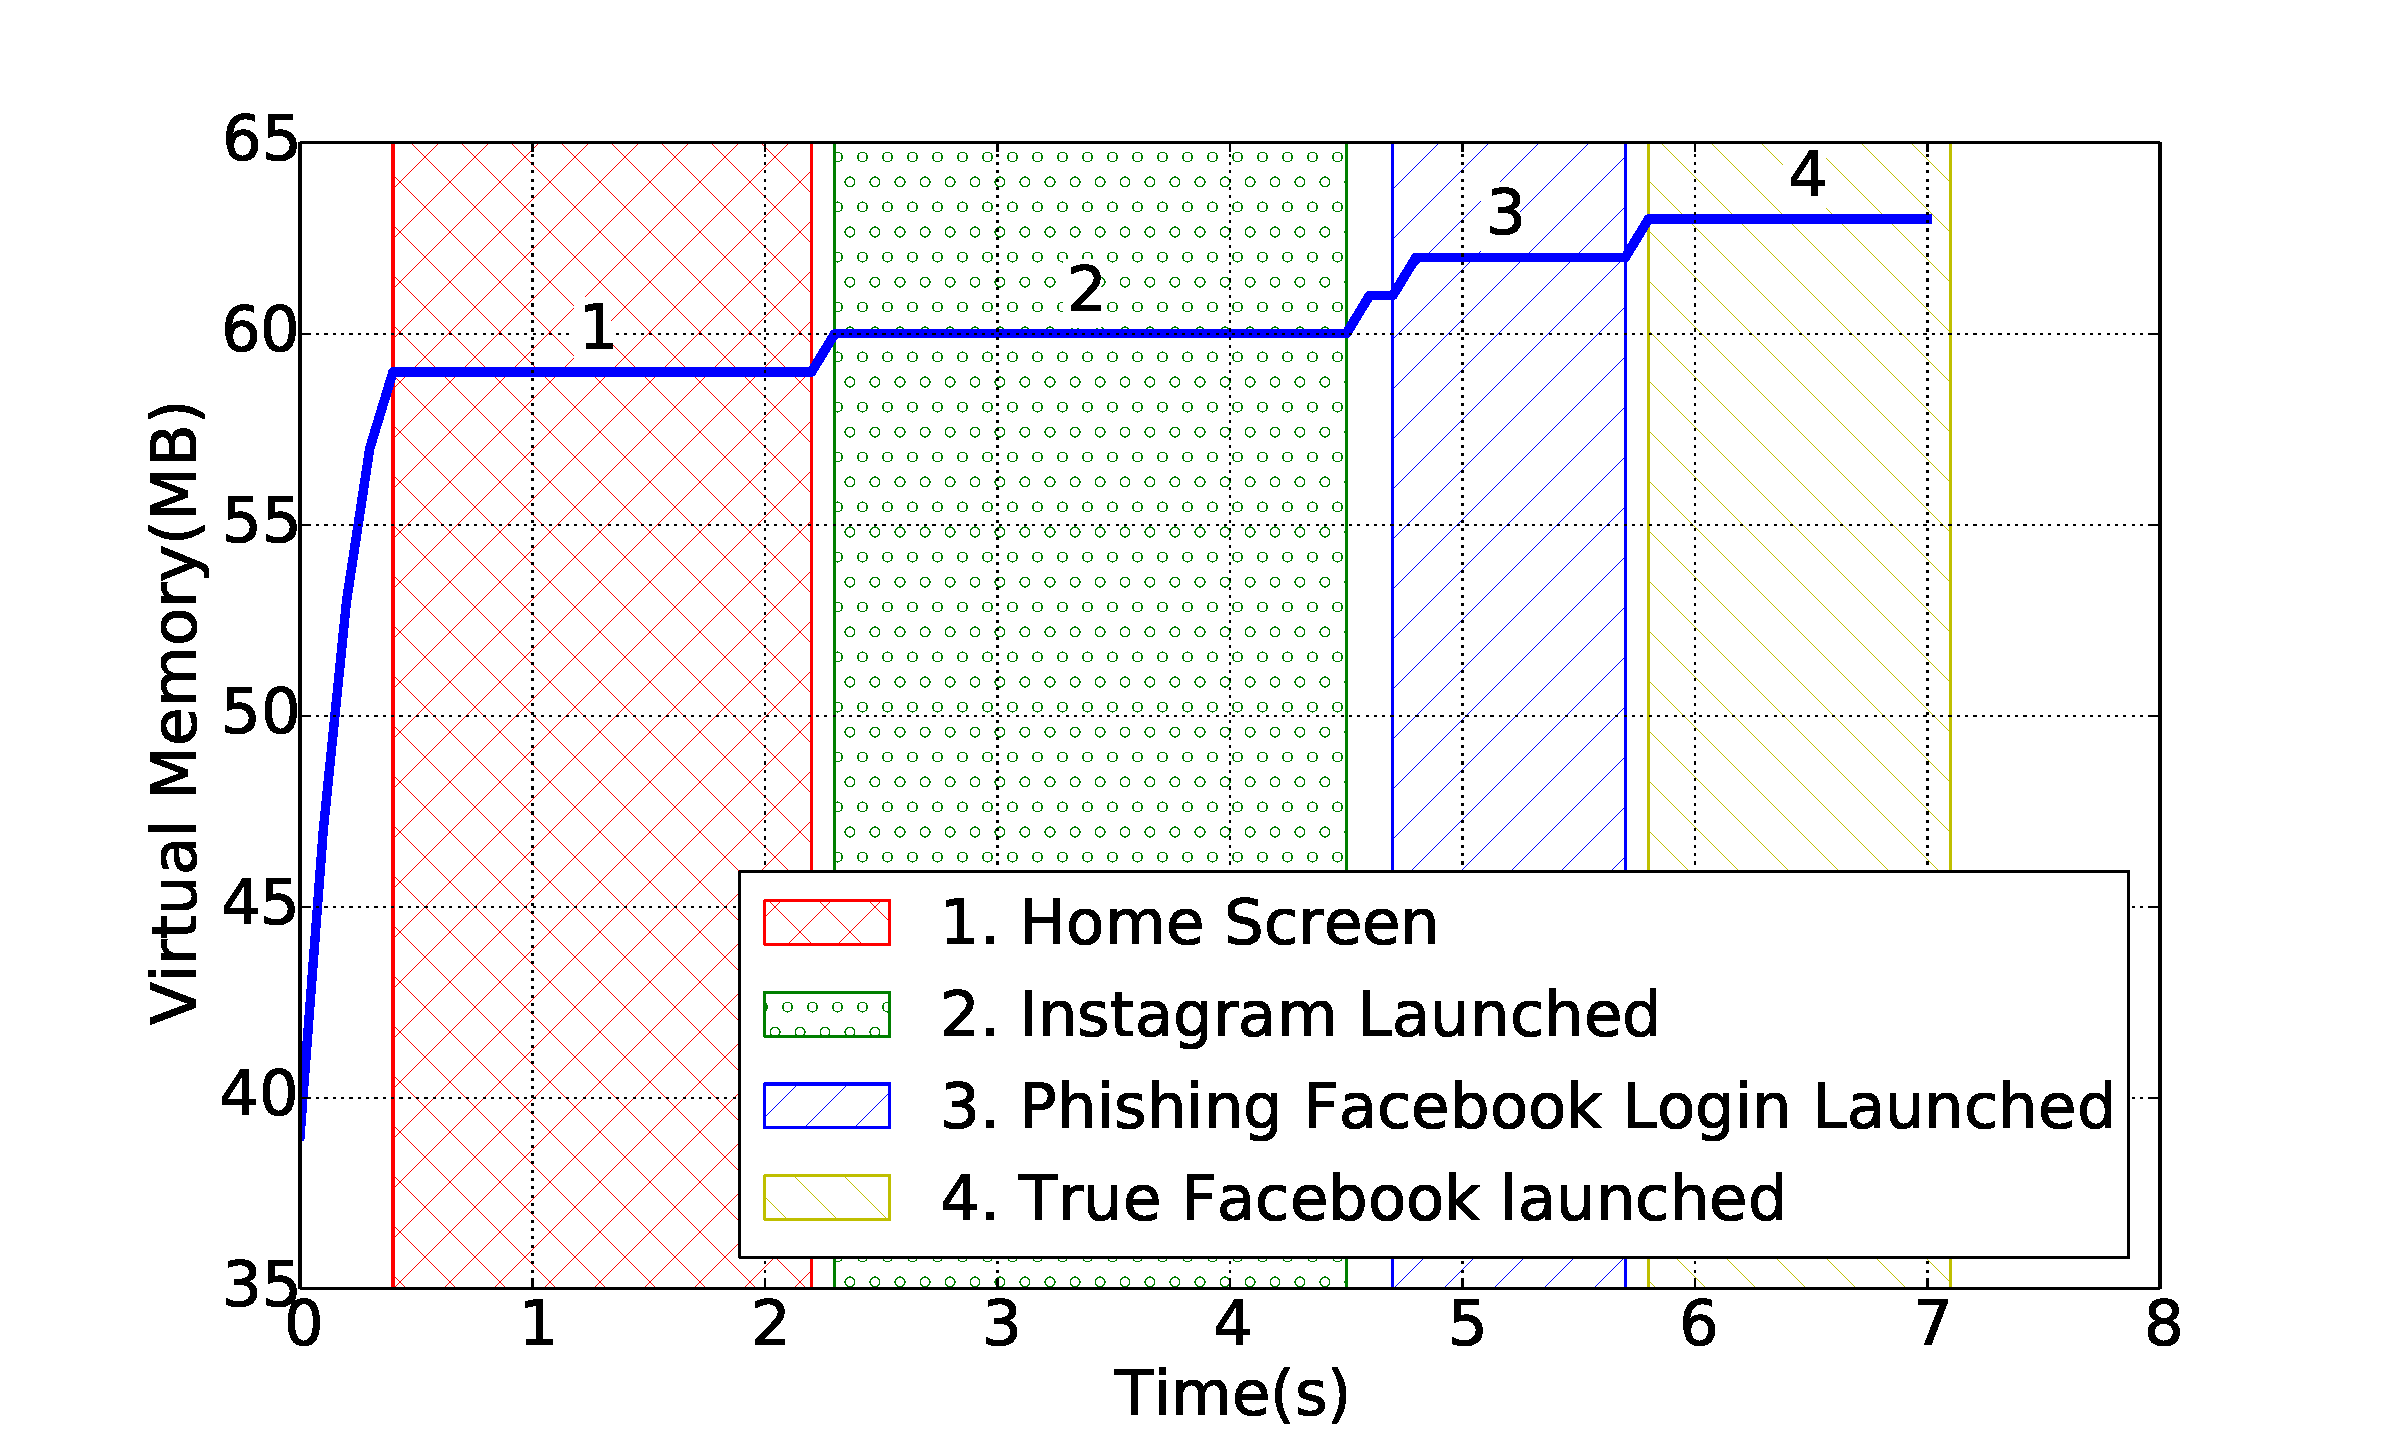
\includegraphics[width=\linewidth]{attack1memory.pdf}
                \caption{UI Phishing}
        \end{subfigure}%
        %\quad
        \begin{subfigure}[t]{0.5\textwidth}
                \centering
          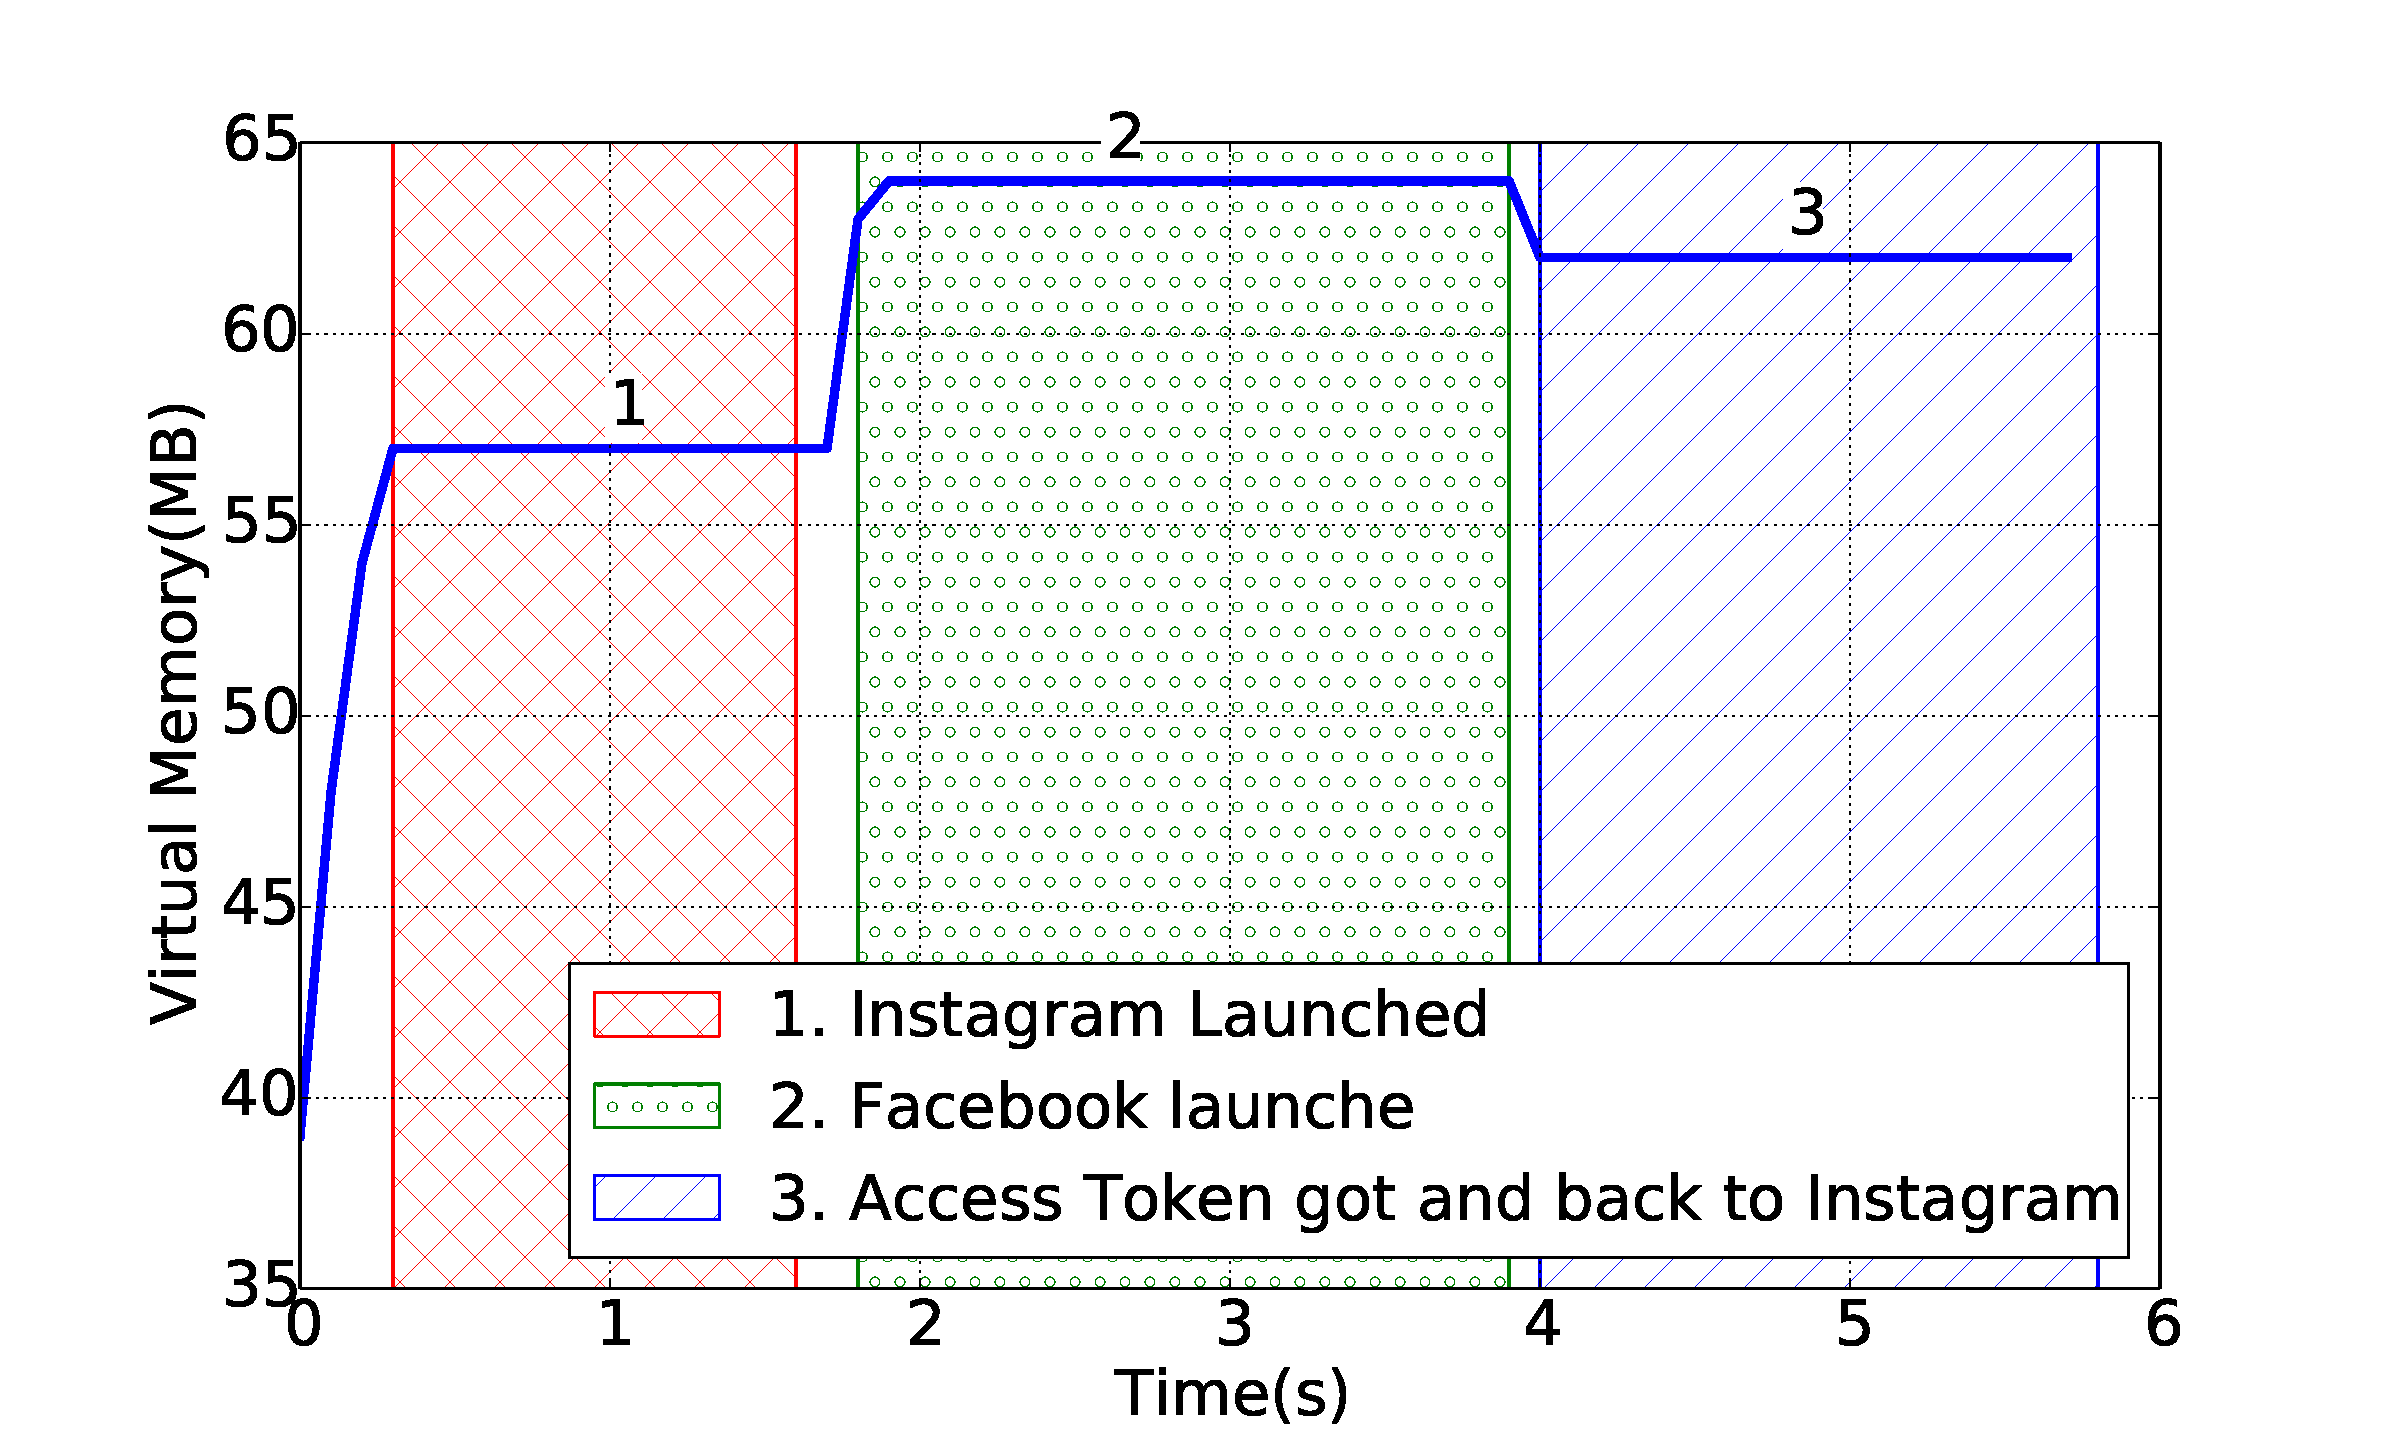
\includegraphics[width=\linewidth]{attack2memory.pdf}
                \caption{Activity-in-the-middle}
        \end{subfigure}
        \begin{subfigure}[t]{0.5\textwidth}
                \centering
          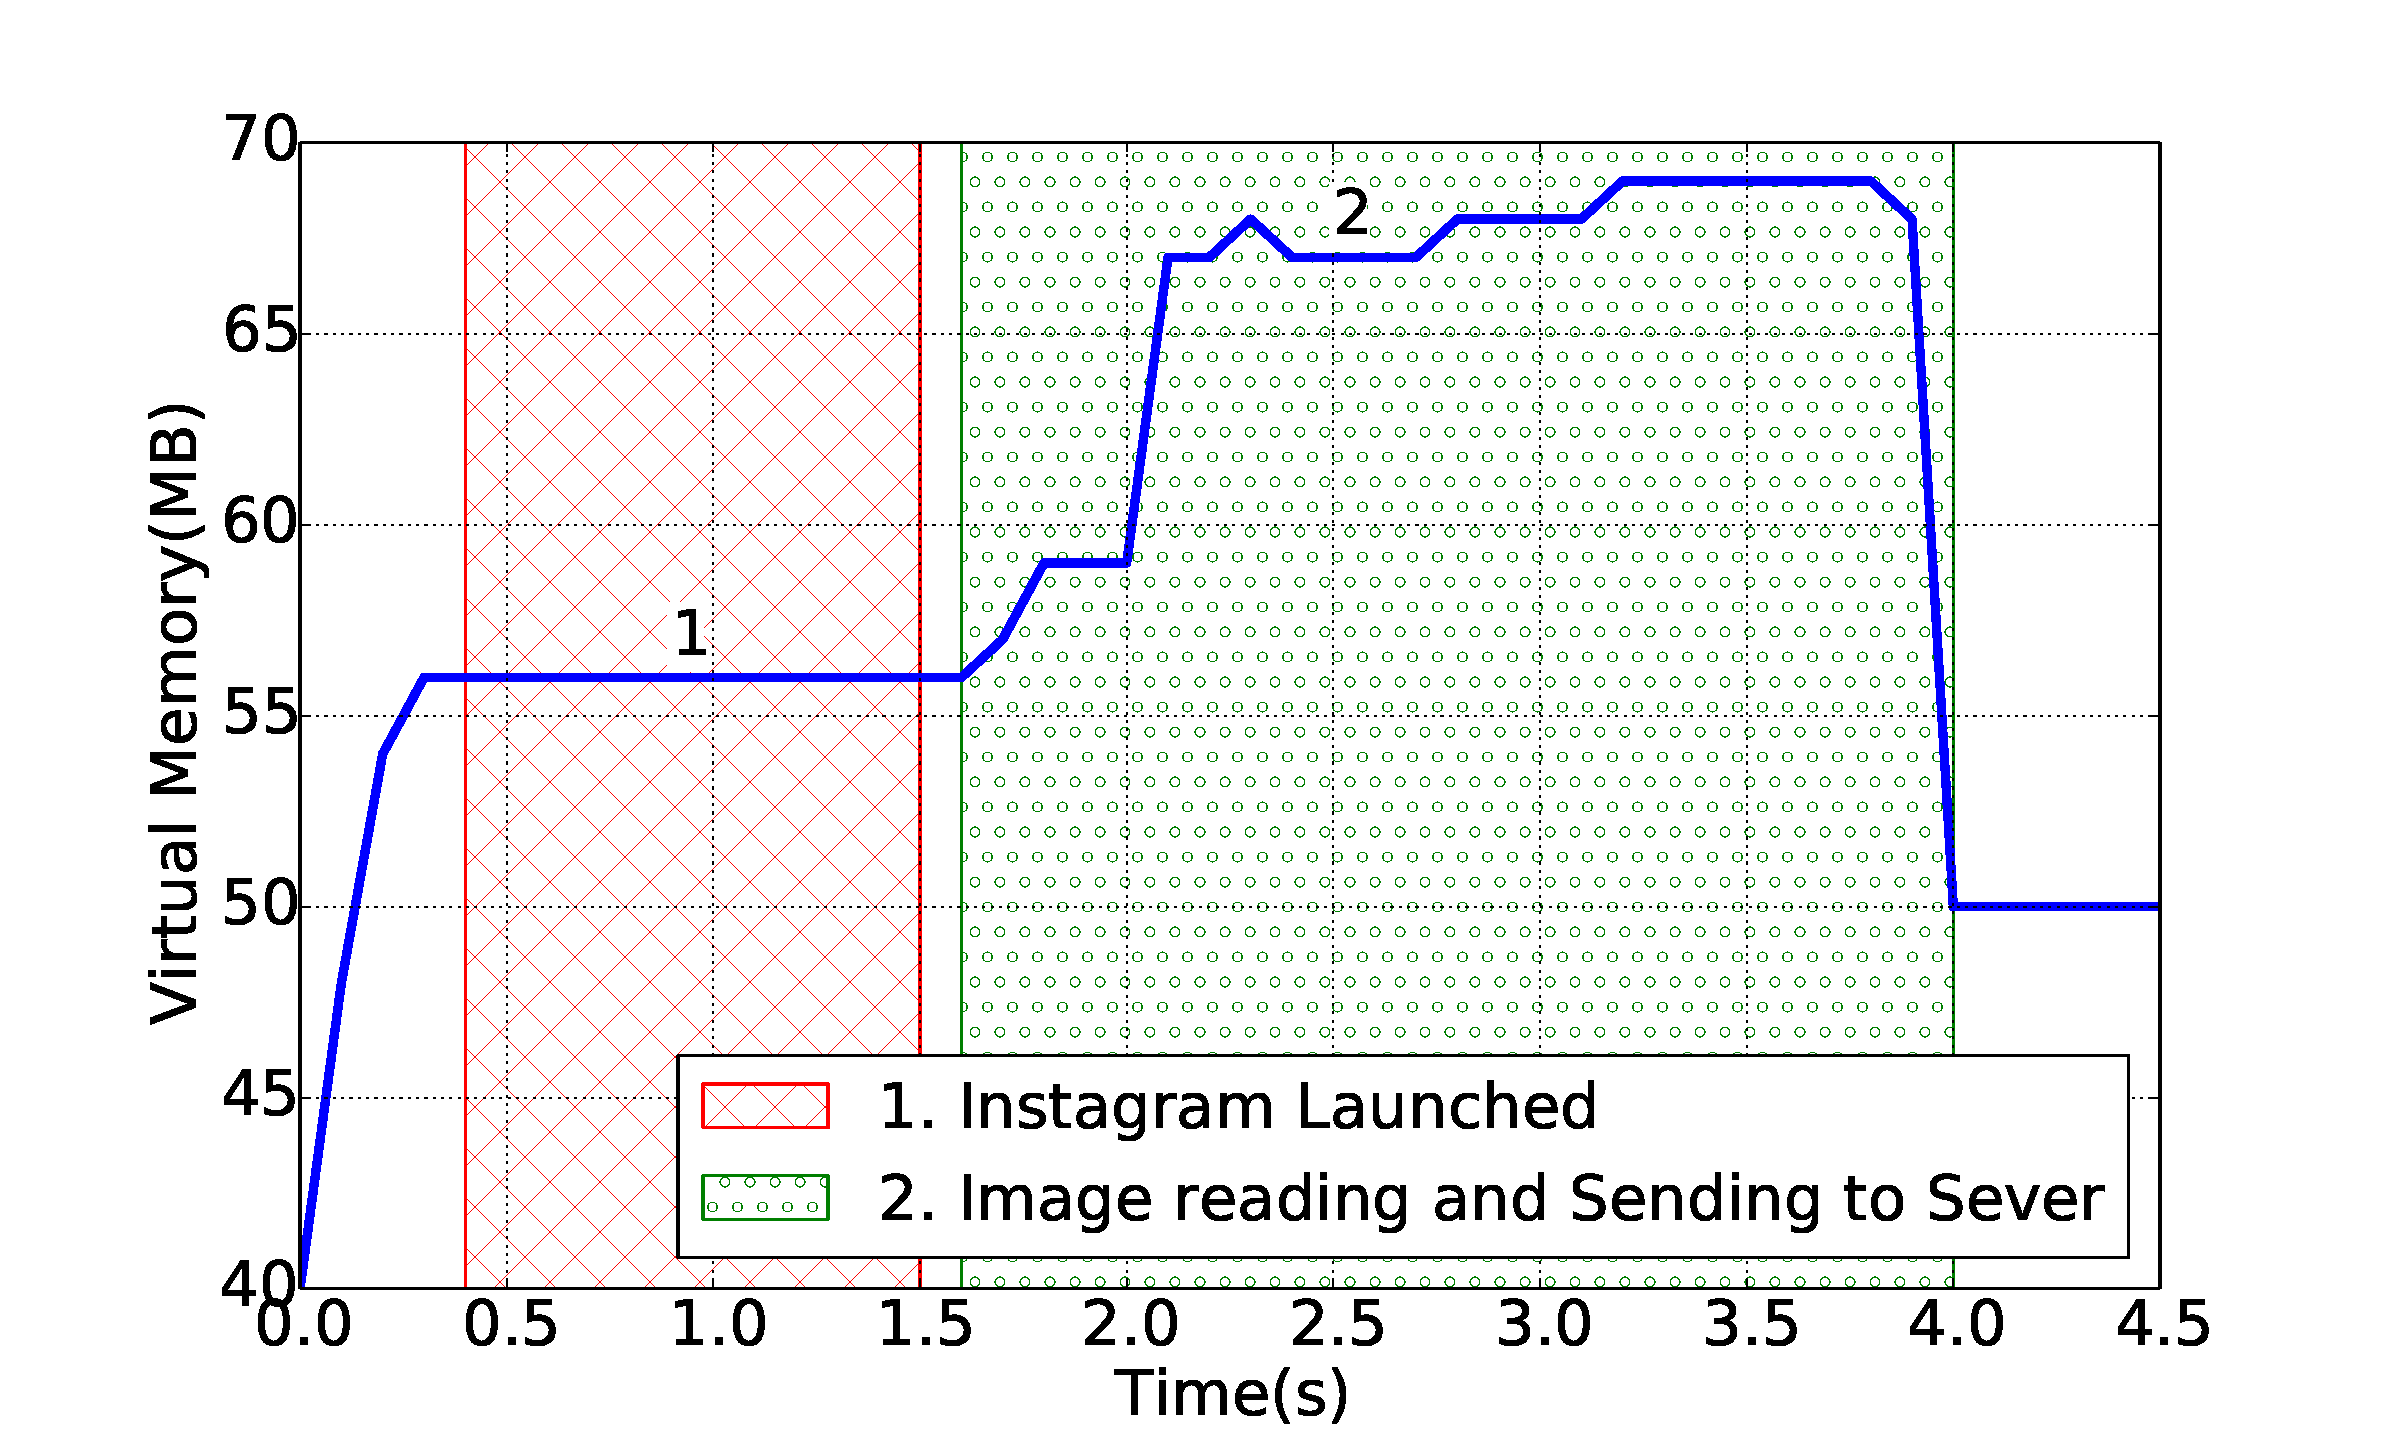
\includegraphics[width=\linewidth]{attack4memory.pdf}
                \caption{Gallery Stealing}
        \end{subfigure}%
        %\quad
        \begin{subfigure}[t]{0.5\textwidth}
                \centering
          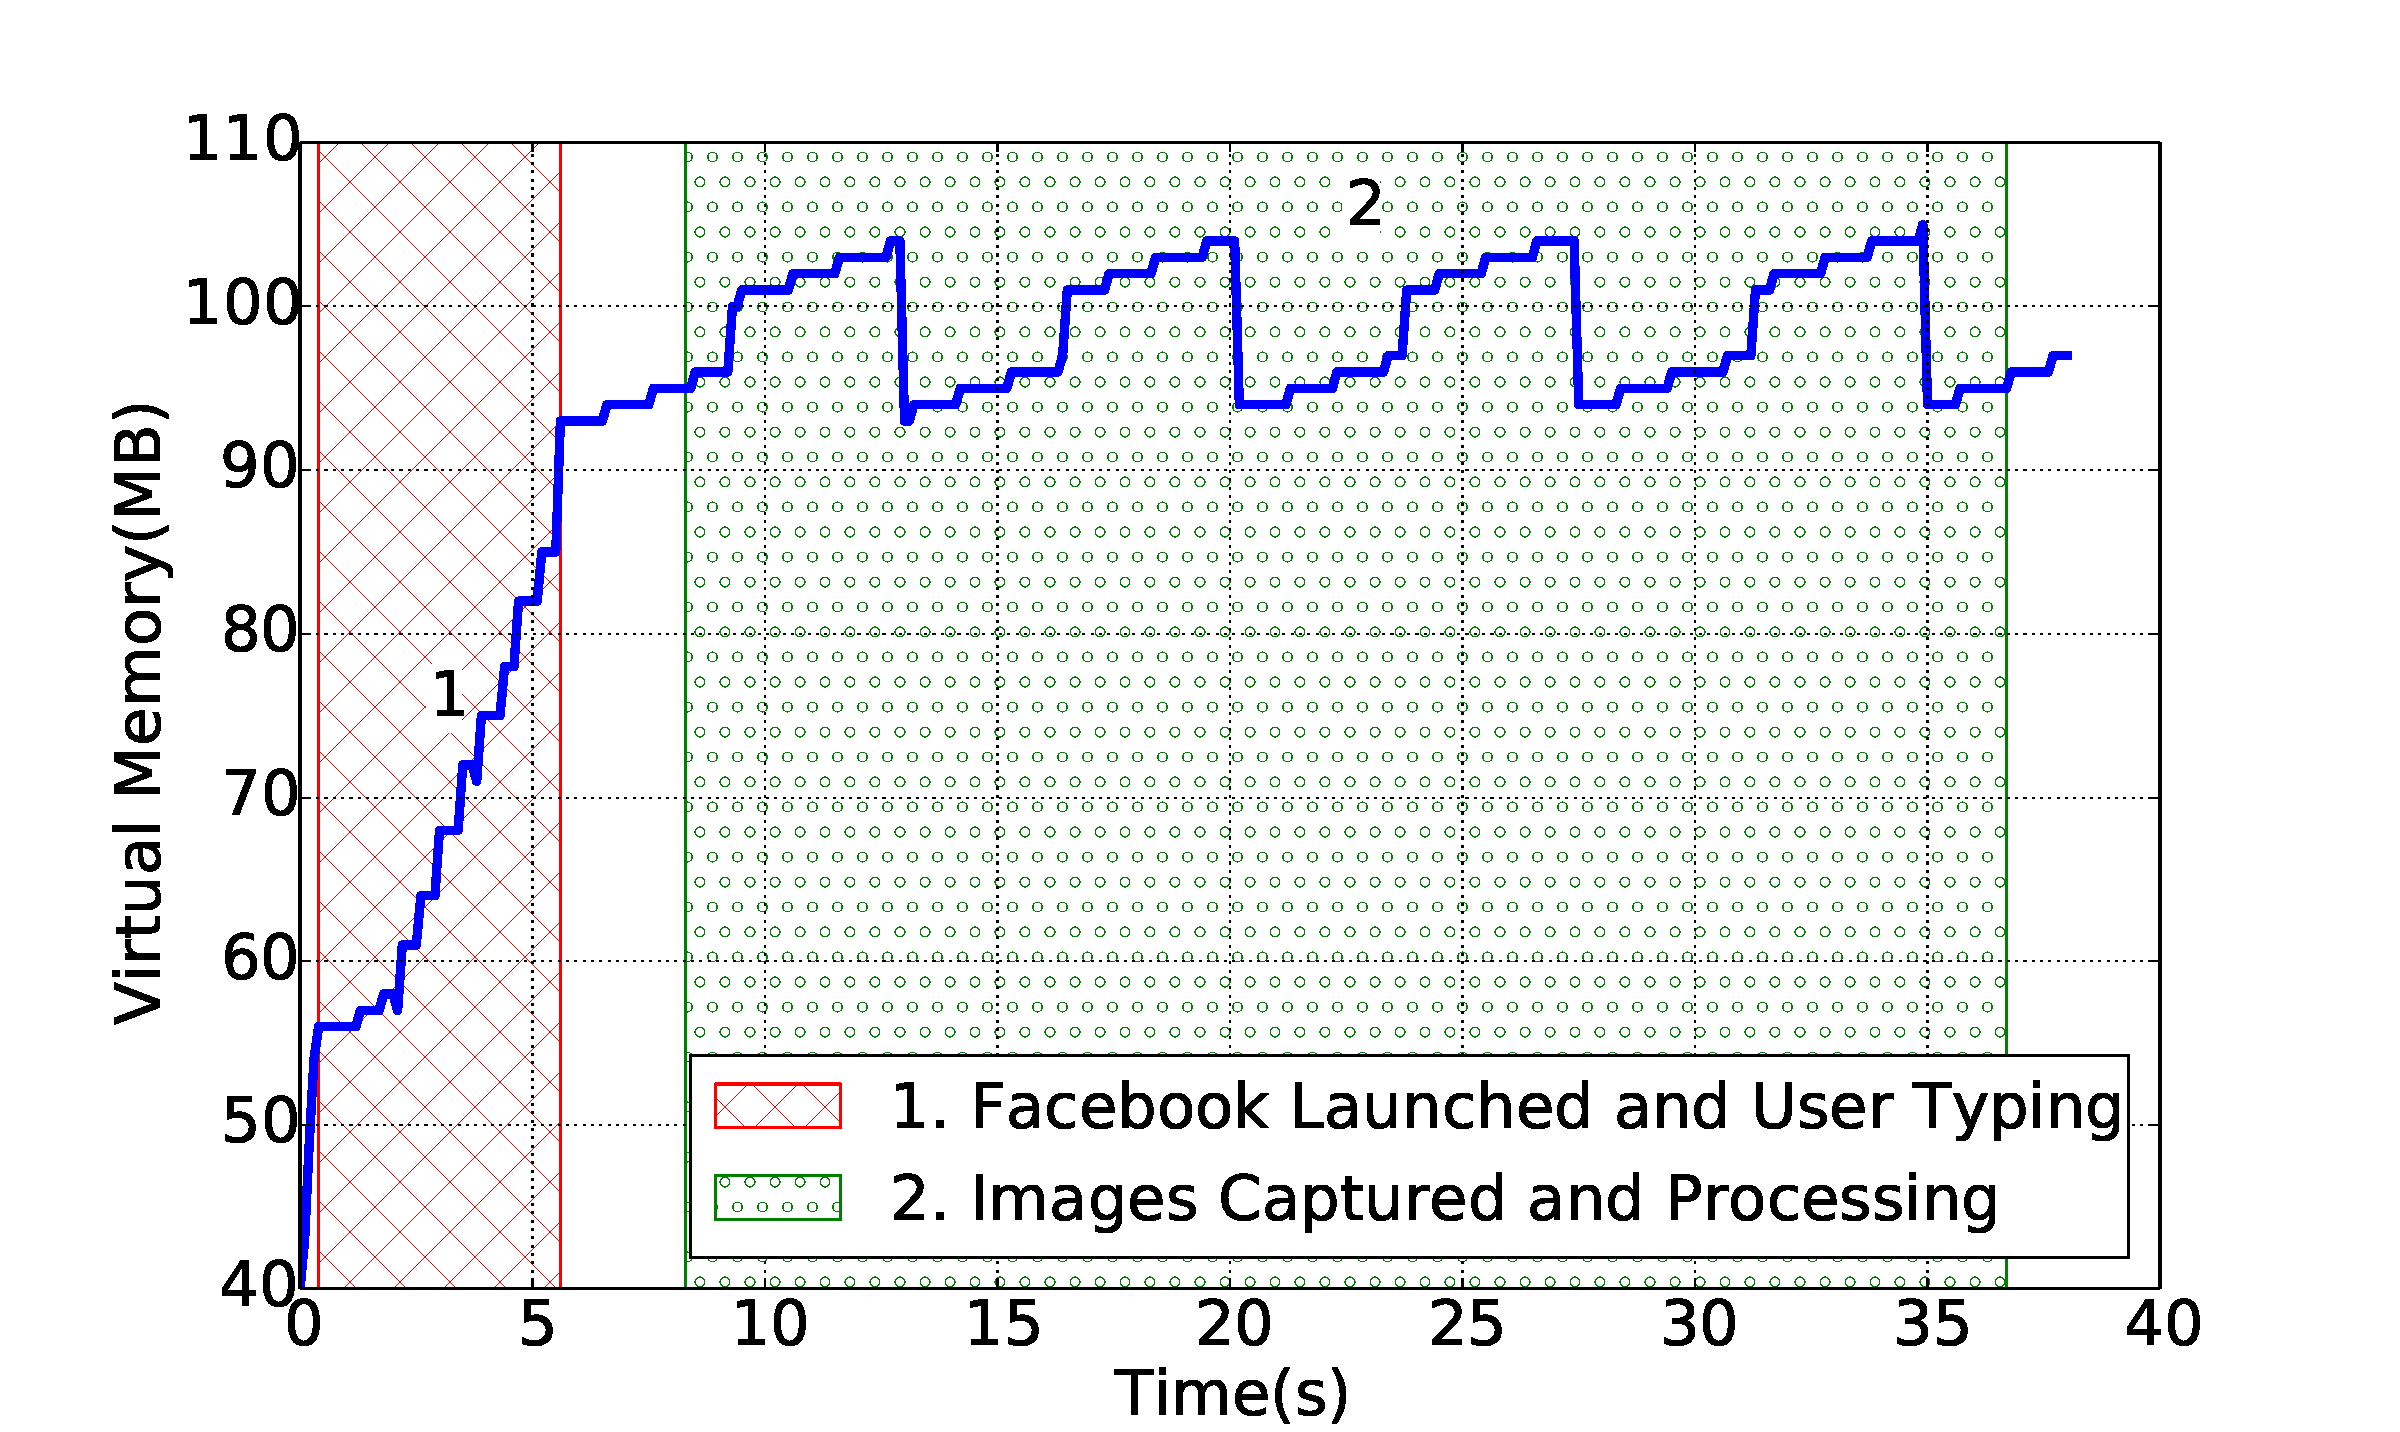
\includegraphics[width=\linewidth]{attack3memory.pdf}
                \caption{Screenshot Capturing}
        \end{subfigure}
         \caption{Memory Distribution Curves}
         \label{fig:memory}
\end{figure}

In addition, we also conduct experiment to monitor the battery consuming
status and evaluate the battery usage of our attacks. The results show
that our attacks may not cause influence on battery aspect (the
battery usage rates of most attacks are $0\%$).  Above all, the
experiment results demonstrate that our proof-of-concept attacks are
light-weight with limited permission requirements.

\subsection{Solutions to Eliminate Task Interference}\label{sec:atmsolution}
In this subsection, we discuss solutions on mitigating Android task
interference. Based on our study, we design and implement a task
interference checking tool to detect the potential risk of task
interference among apps. It protects apps specified by users from
being manipulated by untrustworthy apps. In addition, we also propose
some suggestions to limit the additional privilege achieved by the
apps in the same task.

\subsubsection{Task Interference Checking}
\label{sec:implementation}
In this subsection, we present the design and implementation of our
\textsl{Task Interference Checking} app named \textsl{TICK}.

Based on our understanding of the task interference problem, which
includes the necessary conditions, events and their dependency, we
design a method to check the task interference status among Android
apps.  Table~\ref{tbl:taskinterference} provides us with the basis of
evaluating task interference checking.

\begin{figure*}[t]
        \centering
                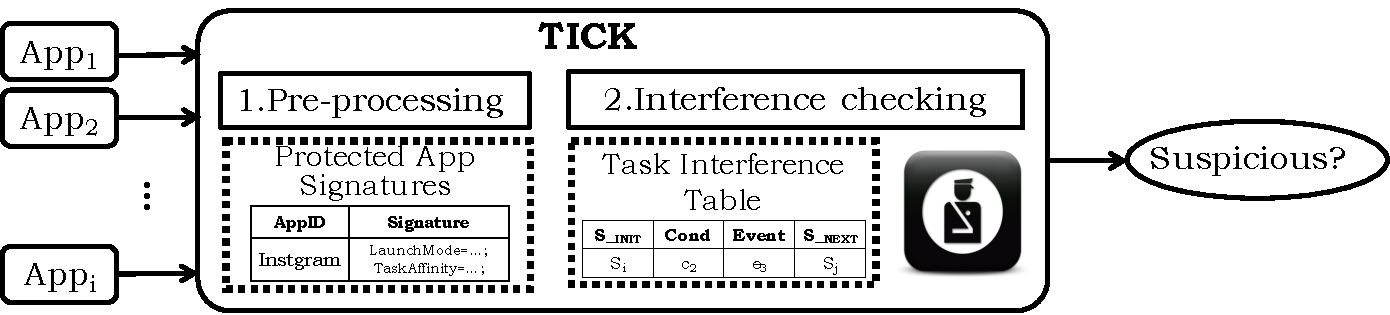
\includegraphics[width=\linewidth]{tick.pdf}
           \caption{Task Interference Checking Architecture}
           \vspace{-0.2cm}
        \label{fig:tick}
\end{figure*}

\textbf{Design.} As shown in Figure~\ref{fig:tick}, \textsl{TICK}
consists of two basic modules, \textsl{Pre-processing} and
\textsl{Interference Checking}, and two supporting databases,
\textsl{Protected App Signature} and \textsl{Task Interference Table}.

\begin{itemize}
\item \textsl{Protected App Signature.} For the apps users who want to
  protect against attacks to Android tasks, this database includes the
  abstracted conditions of such attacks of each app, which is stored as
  signatures in this database.
\item \textsl{Task Interference Table.} This database is the output
  from our research in Section~\ref{sec:atmapproach}, which includes the
  fundamental rules of task interference.
\item \textsl{Pre-processing.} The module takes as inputs the manifest
  files of apps to be checked, abstracts and outputs their task
  interference features for checking.
\item \textsl{Interference Checking.} The interference checking module
  takes inputs from \textsl{Pre-processing} module and \textsl{Protected App
  Signature} database, and checks the suspiciousness of the testing apps
  according to the rules specified in the Task Interference Table.
\end{itemize}

There are two application scenarios for deploying \textsl{TICK}.
\begin{description}

\item[\textbf{C-1:}] Before a user installs an app, she/he can use
  TICK to detect the potential risk of task-related attacks from the app.  TICK
  will parse the app meta data and check with our table and signature
  database to see if it interferes with an existing app. If the app is
  detected to cause interference, TICK will issue a
  warning to the user and suggest she/he not install the app.
\item[\textbf{C-2:}] Our checking app can do chronically scan from
  time to time, check if new packages are added to the device, audit
  if they have security concerns, and notify users if and suspicious
  package were installed.
\end{description}

\textbf{Getting Meta Data of an Activity.}  Currently, our checking app
only considers static declarations of task related attributes from the
app package. Moreover, the key attributes related to Android Task
cannot be altered during runtime, e.g., \textit{taskAffinity} and
\textit{allowTaskReparenting}.

Android SDK provides standard APIs to get an app's Manifest meta data
without requiring any permission. Given a package name and a flag, one
can retrieve an object of \texttt{PackageInfo} through the
\texttt{PackageManager}. Here, we set the flag to
\texttt{GET\_ACTIVITIES} and we retrieve a list of
\texttt{ActivityInfo} by fetching the attribute
\texttt{PackageInfo.activities}. ActivityInfo contains all the meta
data described in the \texttt{Manifest} about every activity of a
package, including those we care, e.g., \texttt{taskAffinity},
\texttt{FLAG\_ALLOW\_TASK\_REPARENTING}, \texttt{LAUNCH\_SINGLE\_TASK}
and so on. The key APIs of getting \texttt{packageManager} and
\texttt{packageInfo} are respectively \texttt{getPackageManager()} and
\texttt{getPackageInfo()}.


\textbf{Effectiveness.} To verify the effectiveness, we used Instagram and our UI-Phishing app
as inputs to TICK. It parsed the meta data of each activity in both
apps and found that most activities of Instagram with {\em
  taskAffinity} set to ``com.instagram.android'', while the rest has
{\em taskAffinity} of
``com.instagram.android.ShareHandlerActivity''. Most of the activities
in Instagram have {\em launchMode} set to ``standard''. A small
portion of the activities have the {\em launchMode} set to
``singleTop'', e.g., the \texttt{LoginActivity}. Very few activities
have {\em launchMode} set to ``singleInstance''. The UI-Phishing app's
first activity has the following flags set: \texttt{taskAffinity =
  "com.instagram.android"}, \texttt{allowTaskReparenting = true} and
\texttt{launchMode = standard}. This matches Case 9 and Case 10 in our
task interference table. When we use TICK to scan the device,
specifying the Instagram app as the one to be protected, TICK
successfully warns users about the potential risk from the UI-Phishing
app. The overhead of TICK can vary based on a number of factors such as device hardware and number of third-party Apps installed in the device. In our experiment, excluding all system-level Apps, there are totally 65 third-party Apps installed in our device. It rougly took 4-5 seconds to scan all Apps and identify suspicious ones.

\subsubsection{Design Suggestions}

From security issues we have demonstrated in the above attacks, it is
clear that the privilege given to apps in the same task is well beyond
what is expected for a mechanism that facilitates app collaboration
and interaction. In fact, the task mechanism should be treated as a
way of {\em authorization}, and the security mechanism around the task
mechanism also should be designed accordingly.

In particular, when treating a task as a boundary for authorization,
we need to be explicit about the ownership of a task and its
authenticity. For example, if an app specifies the {\em taskAffinity}
of an existing task, there needs to be a form of {\em authorization}
before the app can be included into the task, and the authorization
should be carried out by entities with privilege greater than the
privilege given to the task. This is similar to the requirement made
by the UNIX group mechanism. In addition, as the name of ``task affinity''
becomes an identifier for a security object, the system should avoid
name conflicts. In case they occur, they need to be resolved with all
involving entities to avoid unexpected privilege escalation.

\subsection{Related Works}\label{sec:atmrelated}
\textbf{IPC Security:} IPC security is one of the top concerns while
designing OSes. Some early studies have reported security threats in
the Android IPC mechanism. More specifically, Ren
et al.~\cite{TaskHijacking} have proposed the first study of the
security of Android task mechanisms and showed the possibilities of
several enabled attacks, such as back-button hijacking and
uninstalling-prevention attack. Other popular mobile systems like iOS
are also not immune to the risks. Xing et al.~\cite{CrackingiOS}
registered a counterfeit scheme which hijacks the real Facebook scheme
in iOS and successfully stole a Facebook access token that was
supposed to be passed onto the relying-party app. Besides problematic
designs of IPC of OSes, mis-implementation of certain IPC-based
protocols can also lead to security concerns. Chen
et al.~\cite{OAuthDemystified} have conducted an analysis on 149
mobile applications and showed 89 of them (59.7\%) incorrectly
implemented OAuth and thus are vulnerable to SSO-oriented attacks.
Furthermore, IPC vulnerabilities were also documented on other
platforms besides mobile OSes. Take browser platform for an example.
Wang et al.~\cite{webssoattack} discovered 8 serious logic flaws among
the traffics between high-profile ID provider and relying website
through browser platform. Wang et al.~\cite{shopforfree} discovered
logic flaws in several shopping websites and finally purchasing goods
without or with little payment.

\textbf{GUI Security:} As for traditional desktop and browser
environment, GUI security issues have been studied
extensively~\cite{nitpickers,secuserinterface}. Niemietz
et al~\cite{uiredress} implement a UI redressing attacks on Android
devices base on clickingjacking and tapjacking and the attack is
feasible to be transferred from desktop to mobile and to browser,
enabling the attack to be adapted to multiple platforms and
functionalities. As mobile market begins to thrive, GUI security is
more concerned in mobile platforms than ever before. Chen
et al.~\cite{UIstateinference} managed to impose Hidden Markov Model
(HMM) on a public resource \texttt{shared\_vm} combining a bundle of
data to perform UI Inference Attack and successfully stole sensitive
information from users such as user names, passwords and check images.
Wang et al.~\cite{jekyll} implemented a malicious app which
circumvented the Apple Code Review system and successfully stole user
secrets stealthily. 

\textbf{Defending against Malicious Behaviors:} Defending malicious
behaviors can be categorized into two branches, detection and
prevention. In previous studies, various detection schemes have been
introduced to prevent GUI-related attacks. Fu
et al.~\cite{detectpswebsite} employ the Earth mover's distance (EMD)
mechanism to detect possible malicious web page through measuring the
similarity between two web pages by first converting web pages to
images, and then grabbing and comparing the feature points through
training data set. More generally, Chen et al~\cite{peg} introduce the
concept of permission event graph (PEG) with model checking mechanisms
to detect abnormal behaviours of Android apps. As for prevention, one
idea is to prevent sensitive data from being leaked to the malicious
server party. Hornyack et al.~\cite{AppFence} develop a
system for Android called AppFence, which can block the sensitive data
from being transmitted, or substitute the fine-grained data to
coarse-grained data if transmission is unpreventable. Ren
et al.~\cite{Windowguard} develop WindowGuard which protect against GUI
attacks by enforcing the Android Window Integrity (AWI).

   \newpage
   \begin{singlespace}
   \section{A Novel Attack Architecture for Device-Identity Association based on Android Side-Channels}
   \end{singlespace}
   \label{sec:dssnassociate}
   
   \subsection{Threat Model and Approach Overview}\label{sec:dssnthreatapproach}
   In this subsection, we present the threat model and the overview of our attack approach.

\subsubsection{Threat Model}\label{sec:dssnthreat}
We consider an attacker who can accomplish inference attacks through a malicious app installed on a victim's device with no special permission -- this malicious app only requests the \texttt{INTERNET} permission from Android to send the collected data to the attacker for analysis, which by default is automatically granted by the Android system without notifying the user. How to install a malicious app in a victim's device is out of the scope of this work. Here are a few viable approaches: an attacker can trick a user to install a malicious app by simply disguising the app as a benign one and putting it on the Google Play Store since current automatic malware detection for Android is still not sufficiently reliable \cite{googleplaymalware}; alternatively, an attacker can secretly install a malicious app on a victim's device by exploiting a remote code execution (RCE) vulnerability such as CVE-2017-0561, which allows RCE on Wi-Fi SoC \cite{wifirce}. In this work, we assume that a malicious app has already been installed on the victim's device. This malicious app can silently collect and send to the attacker certain system states that are publicly available.

\subsubsection{Approach Overview}\label{sec:dssnapproachoverview}
The objective of our design is to associate an Android device (running social network apps to perform social activities such as posting a photo or a message) with the social network accounts (the accounts accessed by the device) based on the following publicly available information: (i) the system state information (see Section~\ref{sec:preliminaries}) collected by a malicious app installed in the victim Android device; and (ii) the social network events crawled from the social network databases. We consider three popular social networks: Twitter, Flickr, and Instagram, and exploit the tweeting events in Twitter and photo-posting events in Flickr and Instagram for our studies on device-identity association. 

\begin{figure}[!htb]
  \centering
    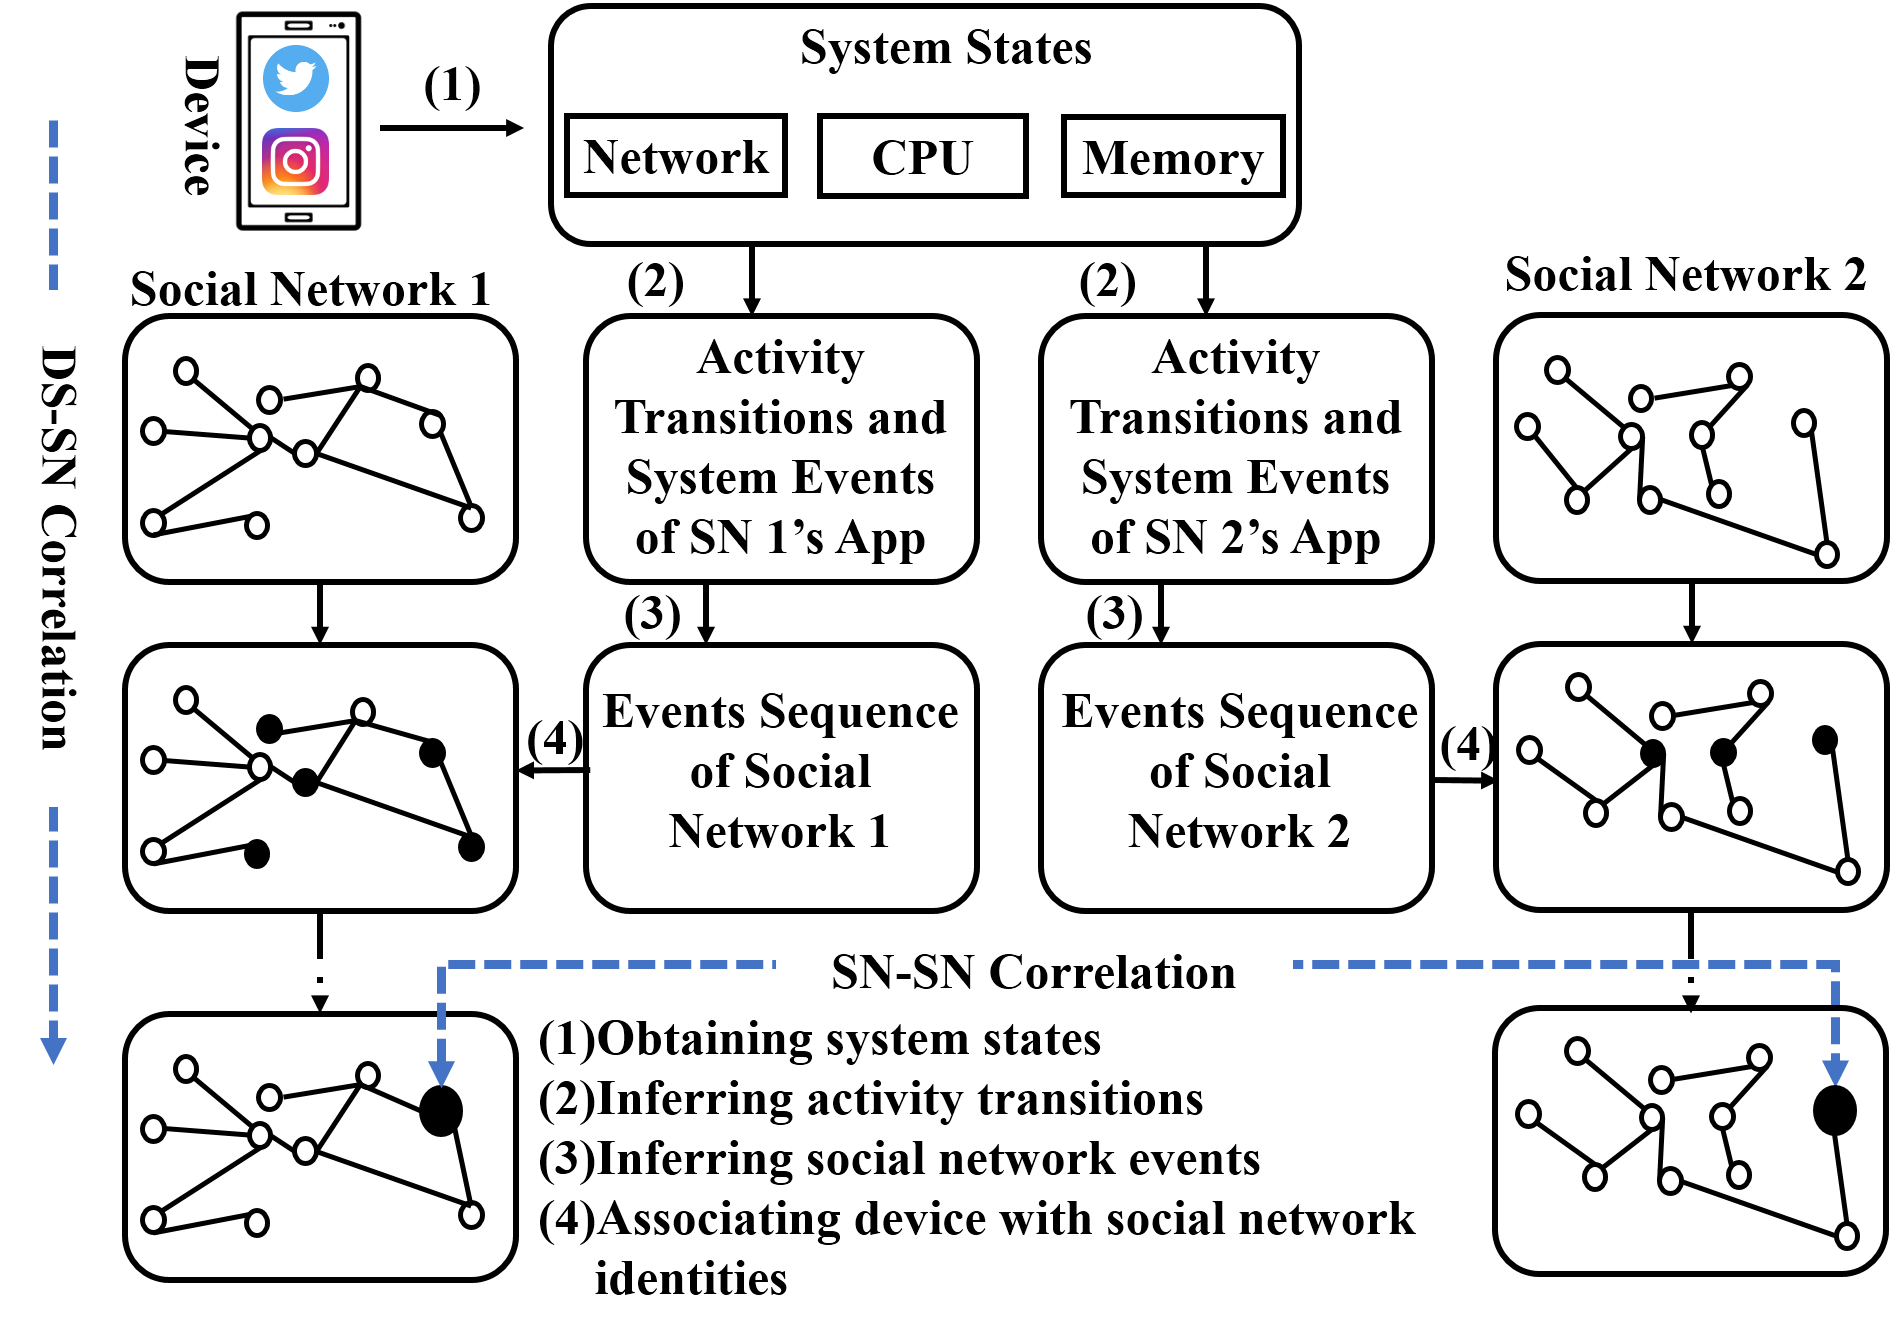
\includegraphics[width=\textwidth]{overview.png}
    \caption{Attack Architecture}
    \label{fig:overall}
\end{figure}

Our attack architecture is shown in Figure~\ref{fig:overall}. It is composed of two attack vectors: \emph{device-social network correlation (DS-SN)} attack and \emph{social network-social network correlation (SN-SN)} attack. The objective of the DS-SN attack is to identify a list of candidate accounts that might have been accessed via the device for a target social network. We developed an approach to infer a user's social network events from his device system states. More specifically, we leveraged the system states collected by a zero-permission malicious app installed in the user's device to identify the events triggered by the social network app, e.g., the time to tweet and the size of the tweet in Twitter, or the time of posting a photo in Flickr/Instagram. By correlating such information with the public events in the target social network, one can identify a list of candidate accounts in the social network for the user who may have used the device to access his account. To uniquely identify the social network account accessed via the device, one can observe multiple social network events triggered by the device to shorten the candidate account list, which may take a long time if the user does not frequently access his account via the device. If the device is used to access multiple accounts of the same user belonging to different social networks, the attacker can employ the SN-SN attack that examines the profile similarity between two social network accounts from two different social networks to identify the most possible account for the user in each social network. More specifically, the attacker first obtains the candidate account lists for two (or more) social networks via the DS-SN attack, then calculate the profile similarity of two accounts, with one from each account list, and identify the pair of accounts with the highest similarity. Such a SN-SN attack can not only speedup the process of device-identity association attack, but also help identify two or more social network accounts accessed via the same device for the victim.

\subsection{Design and Implementation of Our Attacks}\label{sec:dssnapproach}
In this subsection, we detail our design of the two inference attacks: DS-SN attack and SN-SN attack.

\begin{table}[!htb]
\centering
\caption{Summary of the DS-SN Attack}
\label{tbl:ds-sn-summary}
\resizebox{\columnwidth}{!}{
\begin{tabular}{|c|c|c|c|}
\hline
\hline
                         & Inferred SN Events                                                            & \begin{tabular}[c]{@{}c@{}}Corresponding \\ Activity Transition\end{tabular} & \begin{tabular}[c]{@{}c@{}}Corresponding\\ System States\end{tabular}                                                                                          \\ \hline \hline
\multirow{2}{*}{Twitter} & Tweeting Timestamp                                                         & \begin{tabular}[c]{@{}c@{}} \texttt{MainActivity}\\ $\Downarrow$\\ \texttt{ComposerActivity}\end{tabular} & \begin{tabular}[c]{@{}c@{}}\emph{VSS} of Twitter\\ \texttt{tcp\_snd} of Twitter\\ \texttt{tcp\_rcv} of Twitter\end{tabular}                              \\ \cline{2-4} 
                         & \begin{tabular}[c]{@{}c@{}}Number of Characters \\ of a Tweet\end{tabular} & N/A                                                                           & \begin{tabular}[c]{@{}c@{}}\texttt{utime} of Keyboard\\ \texttt{stime} of Keyboard\end{tabular}                                                            \\ \hline
Instagram                & Photo-posting Timestamp                                                    &\begin{tabular}[c]{@{}c@{}} \texttt{MediaCaptureActivity I}\\ $\Downarrow$\\ \texttt{MediaCaptureActivity II} \end{tabular}      & \begin{tabular}[c]{@{}c@{}}\emph{VSS} of Instagram\\ \texttt{tcp\_snd} of Instagram\\ \texttt{tcp\_rcv} of Instagram\end{tabular}                        \\ \hline
Flickr                   & Photo-posting Timestamp                                                    & \begin{tabular}[c]{@{}c@{}} \texttt{MainActivity}\\ $\Downarrow$\\ \texttt{FilterUploadActivity}   \end{tabular}    & \begin{tabular}[c]{@{}c@{}}\emph{VSS} of Flickr\\ \emph{RSS} of Media Process\\ \texttt{tcp\_snd} of Flickr\\ \texttt{tcp\_rcv} of Flickr\end{tabular} \\ \hline
\end{tabular}
}
\end{table}

\subsubsection{DS-SN Correlation Attack}\label{sec:dssnattack}
Our approach to attacking the DS-SN correlation is composed of 4 steps: 1) obtaining system states from a victim's device via a zero-permission malicious app, 2) inferring activity transitions in the device, 3) inferring the corresponding social network events triggered by the device, and 4) associating the victim's device with his social network account based on the inferred events triggered by the device and the publicly available events crawled from the target social network. We considered three popular social networks: Twitter, Flickr, and Instagram. Our purpose is to infer the tweeting time of and the number of characters in a tweet for Twitter, the posting time of a photo in Instagram, and the posting time of a photo in Flickr. This inference is based solely on the publicly available information: the Android system states collected by a zero-permission app and the tweeting/photo-posting events crawled from the social network databases. The device state information needed by the DS-SN attack as well as the inferred device activity transitions and social network events for the three social networks are presented in Table~\ref{tbl:ds-sn-summary}.

\textbf{Obtaining System States.}

As shown in Table~\ref{tbl:ds-sn-summary}, we exploited \emph{VSS}, \emph{RSS}, \texttt{utime}, \texttt{stime}, \texttt{tcp\_snd}, and \texttt{tcp\_rcv} for our DS-SN attack. There are multiple ways to obtain these system data in Android, as elaborated in Section~\ref{sec:preliminaries}. The most intuitive way is to make calls to the Android APIs. However, one has to retrieve the three types of data using different APIs, making this method less efficient. To overcome this problem, we first leveraged the ``\texttt{ps}'' command with Android Toolbox \cite{toolbox}, which can return the memory and CPU data in one call; then we directly read the system files \texttt{/proc/uid\_stat/pid/tcp\_snd} and  \texttt{/proc/uid\_stat/pid/tcp\_rcv} to retrieve the network data. 

\begin{figure}[!htb]
  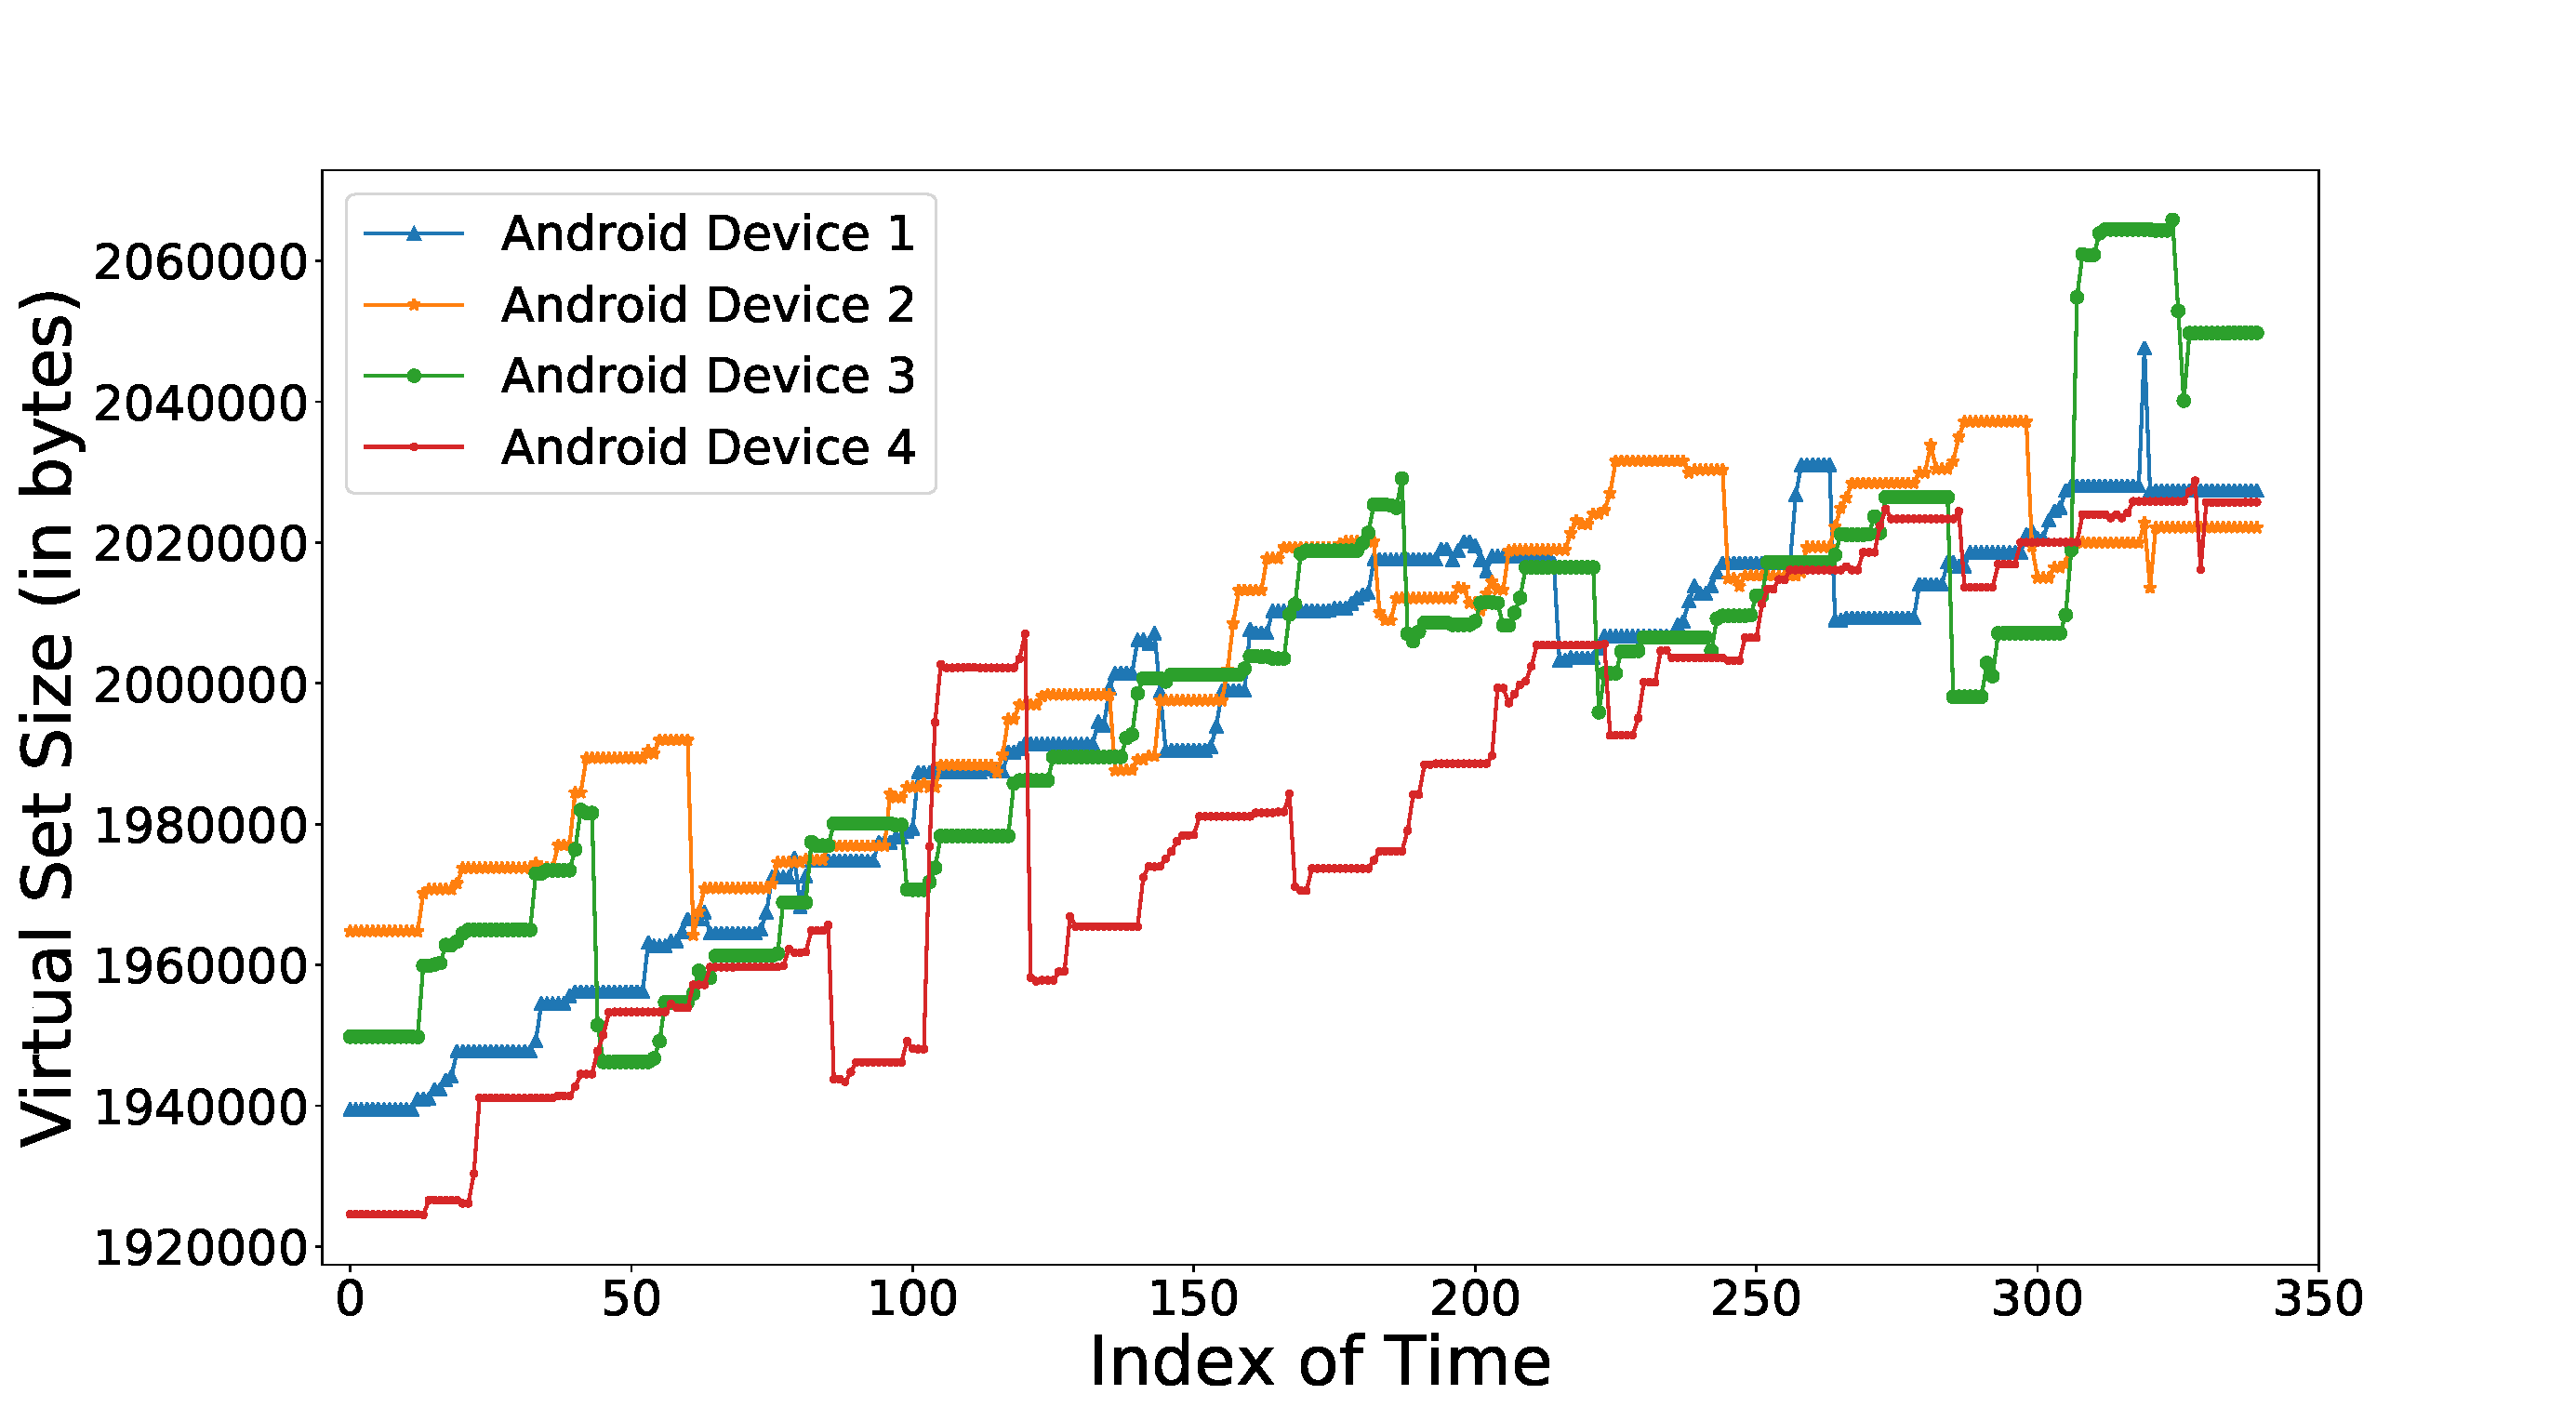
\includegraphics[width=\textwidth]{swipe.pdf}
  \caption{The Variations of \emph{VSS} of the Twitter App}
  \floatfoot{The variations of \emph{VSS} of the Twitter App in four different Android devices within approximately 2 minutes of swiping and tweeting.}
  \label{fig:swipe}
\end{figure}


\textbf{Inference of Activity Transitions}

Activity transition is one of the most critical states to infer private information from an app. Previous research done by Chen \emph{et al.} \cite{chen2014peeking} described an approach that can infer an app's activity transition using a Hidden Markov model (HMM) over the memory data and then further infer the current foreground UI/activity the user is landing on. We tested this approach in our Android devices but failed to make it work. A careful study indicates that this approach is quite sensitive to the quality of the memory data but social network apps when running constantly incur significant noises compared with the clean acctivity transitions considered in \cite{chen2014peeking}. Figure~\ref{fig:swipe} illustrates the variations of the \emph{VSS} of the Twitter app in four Android devices with different OSes when we performed swiping and tweeting for approximately two minutes. Note that people usually swipe when tweet; thus these two activities are commonly performed together. From this study one can conclude that social network apps incur noisy memory data in most Android OSes, and the HMM inference method would face challenges when distinguishing tweeting from swiping. Having noticed this fact, we propose our own approach to precisely infer the activity transitions with the noisy memory data.

To proceed, we take a look at the VSS changes of the three social networks (see Figure~\ref{fig:memory-activity}) when only a posting event is performed - no other activities such as swiping and tapping is involved to remove noise. One can see from Figure \ref{fig:memory-activity} that the activity transition of tweeting (from \texttt{MainActivity} to \texttt{ComposerActivity}) takes 4 time intervals\footnote{Here we refer a time interval as the time span needed for the retrieval of one record of the system states, which can differ from device to device but normally it is within 0.5$\sim$0.6 seconds}; the one for photo-posting in Instagram (from (\texttt{MediaCaptureActivity I} to \texttt{MediaCaptureActivity II}) takes 12 time intervals; while the one for photo-posting in Flickr (from \texttt{MainActivity} to \texttt{FilterUploadActivity}) takes only one time interval. Thus obviously, it is hard to design a uniform approach that can work for all the three social networks. In this subsection, we propose a novel \emph{memory pattern regression} model that can infer the activity transitions based on the VSS variations for Twitter and Instagram, and employ the RSS of the system media process\footnote{We employed RSS for Instagram too but our memory pattern regression model performs better.} to infer the activity changes in Flickr. In the following, we first detail our novel memory pattern regression model. 


\begin{figure}[!htb]
  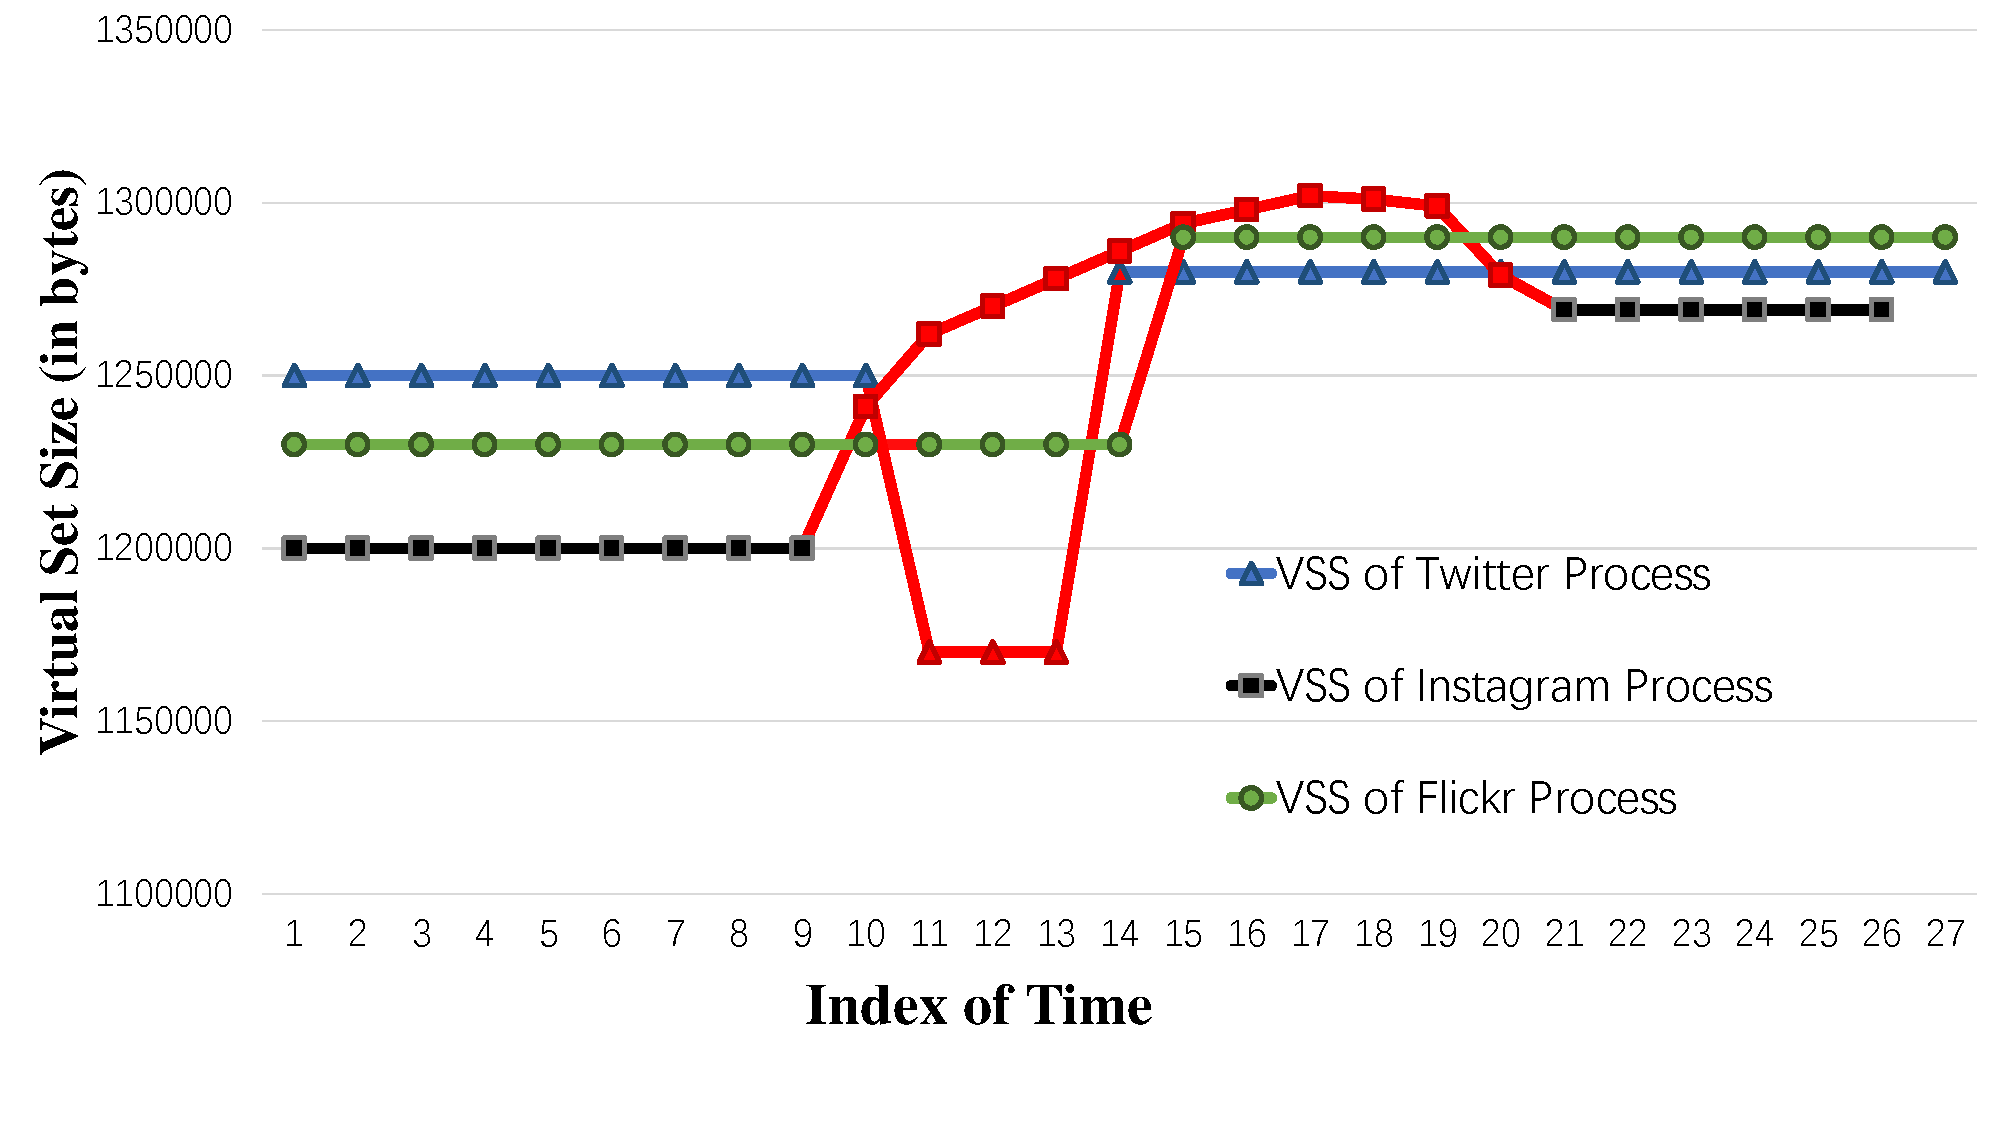
\includegraphics[width=\textwidth]{activity-memory.pdf}
  \caption{The Variations of \emph{VSS} of Twitter, Instagram, and Flickr}
  \floatfoot{The variations of \emph{VSS} of Twitter, Instagram, and Flickr when a tweet or a photo is posted. The red parts refer to the activity transitions of tweeting/photo-posting in the corresponding social network.}
  \label{fig:memory-activity}
\end{figure}


{\noindent \bf Memory pattern regression.}
Our memory pattern regression algorithm takes as input the training set $D=\{\mathbf{y}_j\}_{j=1\cdots d}$, which is the memory data tested $d$ times for a single activity transition with $\mathbf{y}_j = (y_{j_1}, y_{j_2}, \cdots, y_{j_{N_j}})$ being the \emph{VSS} vector of size $N_j$ obtained in the $j$-th experiment. We first need to find out the number $n$, which represents the number of time intervals in which a target activity transition, i.e., an activity transition of a tweeting in Twitter or a photo-posting in Instagram, takes place. In order to determine $n$, we first construct a sequence $\mathbf{\Delta y_j} = (\Delta y_{j_1},\cdots,\Delta y_{j_{N_j-1}})$, where $\Delta y_{j_i}=|y_{j_{i+1}}-y_{j_i}|$; %, and $\mathbf{\Delta y_j}$ has $N-1$ terms since each term of $\mathbf{\Delta y_j}$ is a pair of consecutive terms from $\Delta y_{j_i}$; 
then we set up a threshold $\delta$, which can be determined experimentally, and let $n_j$ be the number of terms in $\mathbf{\Delta y_j}$ whose values are greater than $\delta$; finally %we let $n_j$ be the number of differences between the greatest index and the smallest index of the extracted terms, and
we set $n=\ceil{\frac{\sum_{j=1}^{d} n_j}{d}}$.


Having determined $n$, we proceed to extract the \emph{VSS} change pattern of a transition. Instead of directly using the raw data of \emph{VSS}, we use slopes of each pair of adjacent \emph{VSS} points since doing this can not only mitigate the noises of memory but also obtain the shape of the transition (i.e., pattern). In order to do so, we minimize a function
$f:\mathbb{R}^{n+1}\longrightarrow \mathbb{R}^{n+1}$, which is represented as
%
\begin{equation} \label{eq:msef}
f \leftarrow \argminA_f\{\frac{1}{d}\Sigma^d_{j=1}
[\frac{1}{n}\Sigma^{n}_{i=1}(\Delta f(j_i)-\Delta y^\prime_{j_i})^2]\}
\end{equation}
where $\Delta f(j_i)=f(j_{i+1})-f(j_i)$ 
is the slope between the point $j_{i+1}$ and $j_i$ since $j_{i+1} - j_i=1$, and 
$\Delta y^\prime_{j_i}$ is the $i$th term in the consecutive interval of $\mathbf{\Delta y_j}$ with size $n$ that covers the maximum number of values greater than $\delta$.


In order to learn the $f$ satisfying \eqref{eq:msef}, we employ a 5-layer feedforward neural network with $n$ neurons at each layer. In this deep neural network, each neuron in the input and output layers is connected to a neuron (one-to-one) in the adjacent hidden layers, but all the hidden layers are fully connected. Moreover, the input and output layers simply use the Hadamard product as the activation function while all other layers use the Sinusoid function for activation. 

The neural network adopted in our approach was implemented based on the Google TensorFlow \cite{abadi2016tensorflow} deep learning framework with the Adam stochastic optimization \cite{kingma2014adam} that takes the right part of (\ref{eq:msef}) as a loss function. By minimizing the loss function, we can obtain $\mathbf{v_j}=( \Delta f(j_1),\Delta f(j_2),...,\Delta f(j_{n}))$ as the \emph{VSS} pattern, which is related to an activity transition with $n$ pieces of slopes. 

Let $\mathbf{y}=(y_1,...,y_N)$, with $N>n$, be the \emph{VSS} sequence collected from a victim's device. The question here is: how can we tell whether the target activity transition happens in this sequence based on the pattern $\mathbf{v_j}$? Intuitively, directly determining whether the Euclidean distance  between them is smaller than a threshold $\sigma$, i.e., $\|\mathbf{v_j}-\Delta\mathbf{y}\|<\sigma$ with $\Delta\mathbf{y}$ being $n$  consecutive slops of $\mathbf{y}$, seems reasonable. However, the Euclidean distance is not applicable in our case since if a user constantly uses an app without quitting, the \emph{VSS} of the App would accumulate. Thus clearly, statically setting a threshold can result in a gradually larger error. Therefore, we developed a comparison method which fits our problem well. Instead of directly considering $\Delta\mathbf{y}$, we tolerate a little bit by considering a neighborhood of $\Delta\mathbf{y}$, denoted by $B_{r}(\Delta\mathbf{y})$, where $r$ is a small integer such that $n<r< N$. Specifically, for a \emph{VSS} value at $i$, we consider the previous and post $r$ slopes of this value, yielding $B_{r}(\Delta y_{i})=(\Delta y_{i-r},...,y_{i},...,\Delta y_{i+r})$ (totally $2r+1$ terms). After that, given a threshold $\sigma$, our comparison algorithm extracts each continuous segment of slopes with size $n$ from $B_{r}(\Delta\mathbf{y_j})$ and calculates the mean squared errors with $\mathbf{v_j}$, denoted as $mse_1,mse_2,...,mse_{2r+2-n}$ (totally $2r+2-n$ terms). Lastly, if $\max(|mse_1-mse_2|,|mse_2-mse_3|,...,|mse_{2r+2-n}-mse_{2r+2-n}|)<\sigma$, we perceive that the target activity transition occurs in $B_{r}(\Delta y_{i})$.

For the activity transition inference of the photo-posting event in Flickr, we employed a different approach based on the following observation: when posting a photo in Flickr, a user needs to choose a picture from his album or to take a photo; in this case, the \emph{RSS} of the system media process, i.e., \texttt{android.process.media}, increases and the \emph{VSS} of Flickr increases. Therefore, using this information, one can infer that an activity transition of a photo-posting event occurs in Flickr. Note that even though Instagram is also a photo-based social network, this method does not apply to it because Instagram allows a user to post comments with a picture. Therefore, if directly using this method in Instagram, one may not be able to tell if a user posts a photo or just sends a comment.

\textbf{Inference of Social Network Events}

To infer the timestamp of a tweeting/photo-posting event, we need to check not only the corresponding activity transitions implied by the memory state changes but also the network states of the device: the existence of an activity transition alone does not mean that the event actually has happened - it is completed only after the tweet message or the photo is sent via the network. Therefore, we need to figure out whether \texttt{tcp\_snd} and \texttt{tcp\_rcv} increase after the detection of the activity transition\footnote{One can use only \texttt{tcp\_snd} for the event inference but our experiments indicate that both \texttt{tcp\_snd} and \texttt{tcp\_rcv} increase when an event occurs, which is reasonable as TCP connections involve two-way traffics.}. In other words, an attacker can infer when a tweeting/photo-posting event happens by combining activity transitions with the network \texttt{tcp\_snd} and \texttt{tcp\_rcv} information. 

%\subsubsection{Inference of the Number of Characters in a Tweet Message}
In Twitter, we can also infer the number of characters in a tweet message by the keyboard event. Note that after a tweet is posted, keyboard would disappear and \texttt{tcp\_snd} would increase. However, we cannot use \texttt{tcp\_snd} to precisely estimate the number of characters sent in a tweet due to the protocol overhead of TCP connections. In our approach, we resort to CPU usage information. We found that the system states of the Android keyboard process (\texttt{com.google.android.inputmethod.latin}) are tightly related to a user's typing actions. More specifically, when the keyboard is launched, the \emph{VSS} of the keyboard process increases drastically from a constant state; when a user types a keystroke, the \texttt{utime} and the \texttt{stime} of the keyboard process roughly increase by 1 clock tick. Thus we took the ceiling of the averaged increased clock ticks of \texttt{utime} and \texttt{stime} to estimate the number of characters in a tweet message. %Figure \ref{fig:utime-vtime} illustrates the changes of \texttt{utime} and \texttt{vtime} for a keyboard process. 

\textbf{Associating Device with Social Network Accounts}

After retrieving the targeted social network events based on the Android system states, i.e., the timestamps of the posts and the sizes of the tweets, we can repeatedly match this information with the public information of the target social network to obtain a gradually smaller list of potential social network accounts for the device. For example, from the device system states we inferred that our target victim tweeted twice in two different timestamps and estimated the sizes of these two tweets. Then we proceeded to crawl the Twitter database and filter out those who did not tweet in these two timestamps and whose tweet sizes do not match with our inferred tweet sizes. By this way we can get a reasonably small list of potential Twitter accounts that may be associated with the victim with a high probability. %Similarly, we can carry out the inference attack for Flickr and Instagram.


\textbf{Crawling the Social Network Events}

As mentioned earlier, we need the public information of the target social network to realize the DS-SN attack. More specifically, we need to crawl the tweets/posts occurring at a specific time within a social network. However, it is not trivial to retrieve the required data from the three social networks under our consideration. We have to overcome the following challenges.

First, even though Twitter has a streaming API which provides an interface to facilitate the retrieval of the tweets for a given time period, this method does not work since the API tends to drop a large amount of unimportant data and it has a rate limit. Luckily, we found that Twitter offers a webpage called Twitter Advanced Search (TAS) via which we can retrieve a list of tweets that contain the queried keywords, locations, or user accounts, for a given time period.
Since user accounts are what we want to
retrieve, we cannot use accounts as a filter. Therefore, 
we query with letters from ``a'' to ``z'' as the filtering keywords, 
and the TAS server replies a list of tweets containing any letter from ``a'' to ``z''
with very minimal data loss - the Twitter server fails to return some tweets only when it thinks that these tweets are duplicates or these tweets only contain non-English contents. Hence, we leverage this method by making
queries through TAS with 26 letters and set the time period to be 1 minute.
We wrote a program that sends a url in the following format:
\begin{lstlisting}[basicstyle=\scriptsize]
https://twitter.com/i/search/timeline?f=tweets&vertical=default&q= keyword%20since%3Astart_date%20until%3Aend_date&src=typd&include_available_features=1&include_entities=1&lang=en&max_position=TWEET-old_tweet_id-new_tweet_id-BD1UO2FFu9QAAAAAAAAETAAAAAcAAAASAAAA...A&reset_error_state=false
\end{lstlisting}
where \emph{new\_tweet\_id} is the tweet id of the very first tweet
shown in the result, while \emph{old\_tweet\_id} is the id of the 
last tweet received. Then TAS returns a JSON file containing 20 tweets
for each query sorted by the posting times. Note that this method requires us to recurrently query until we retrieve all the tweets for our desired time period. We
found that in average there are approximately 30,000 - 60,000 new
tweets generated globally at every minute. 

Flickr offers a similar search engine that does not require the inputs of keywords, locations, and so on. In other words, by merely feeding
a time period to the Flickr search engine one can retrieve all the posts
of that time period. Based on our observation, Flickr follows the following format to retrieve posts:
\begin{lstlisting}
https://api.flickr.com/services/rest?sort=relevance&parse_tags=1&content_type=7&extras=can_comment%2Ccount_comments%2Ccount_faves%2'Cdescription%2Cisfavorite%2Clicense%2Cmedia%2Cneeds_interstitial%2Cowner_name%2Cpath_alias%2Crealname%2Crotation%2Curl_c%2Curl_l%2Curl_m%2Curl_n%2Curl_q%2Curl_s%2Curl_sq%2Curl_t%2Curl_z&per_page=100&page=xx&lang=en-US&advanced=1&min_upload_date=start_time&max_upload_date=end_time&viewerNSID=xx&method=flickr.photos.search&'csrf=xx&api_key=xx6&format=json&hermes=1&'hermesClient=1&reqId=xx&nojsoncallback=1'
\end{lstlisting}
where \emph{start\_time} and \emph{end\_time} are Unix times. The
server returns a JSON file containing 100 posts for each requested
page number. Here a page number represents the index of the Flickr post pages, with each page containing 100 posts. For example, the third page (page number three) contains the 301st to the 400th posts following a descending posting time. We wrote a program that keeps on sending the url until all pages have been returned.

In contrast, Instagram does not have any interface for
returning posts based on time; instead, it provides an interface that
returns posts based on locations, accounts, and hashtags. Therefore, we
can only collect as many user accounts as possible for further scrutiny.
Due to the nature of Instagram, almost every
Instagram user follows at least one verified account (celebrity). Thus we
collected all the followers of the official account of Instagram, Selena Gomez, and Taylor Swift, the top three most-followed accounts on
Instagram. As a result, we obtained in total 390,592,786 users while the
number of active Instagram users is about 500 million to 600
million \cite{instdata}. To collect the followers of the three most-followed accounts, we wrote a program that sends a post data to the url \texttt{
\url{https://www.instagram.com/query/}} with the format of
\begin{lstlisting}[language=json,firstnumber=1, basicstyle=\scriptsize]
"q": "ig_user(xxx)
{ followed_by.after(end_cursor, step)
{count,page_info
{ end_cursor, has_next_page}, nodes {id, is_verified,
followed_by_viewer, requested_by_viewer, full_name, profile_pic_url, username}
}
}"
\end{lstlisting}
where \emph{end\_cursor} indicates the cursor of the last retrieved user and \emph{step} indicates the number of users returned at each round.


\subsubsection{SN-SN Correlation Attack}
\label{sec:snsnattack}
Our SN-SN correlation attack is designed to assist the DS-SN attack since the latter may not always be feasible (e.g., taking too long time) due to the infrequency of successive tweets/posts in a single social network by the target victim. To understand this challenge, we carried out a measurement study over 500,008 users randomly selected from the followers of 10 celebrities in Twitter to collect the time intervals between the most recent two successive tweets. As one can see from Figure~\ref{fig:timediff}, over half of these Twitter users tweeted again more than 20 days later after their last tweet. Therefore, if only exploiting the DS-SN correlation, an attacker may have to wait for a long time to collect enough data for a satisfying result. Nevertheless, a user may access different social networks with the same device at different times; thus exploiting the correlations of the accounts in different social networks may help speedup and enhance the accuracy of the device-identity association attack. In this subsection, we investigate the SN-SN correlation to identify the possible accounts in different social networks for the same user, which can help shorten the list of candidate accounts obtained from the DS-SN attack. Assume that an attacker has launched the DS-SN attack on a victim device for two social networks and obtained two lists of candidate accounts. Then the objective of our SN-SN attack is to identify the accounts that can match to the same user with high probability. This is done by the so-called \emph{profile similarity}, which is a weighted average of the similarities of five attributes:  \textit{location} ($s_1$), \textit{personal website link} ($s_2$), \textit{username} ($s_3$), \textit{biography} ($s_4$), and \textit{profile image} ($s_5$). A novel learning-based model is presented to calculate the weight for each attribute.  %Then we define an overall similarity which aggregates all these similarity metrics into a weighted representation. Lastly, we employ a learning-based method to find the weights for overall similarity to refine our results.

\begin{figure}[!htb]
  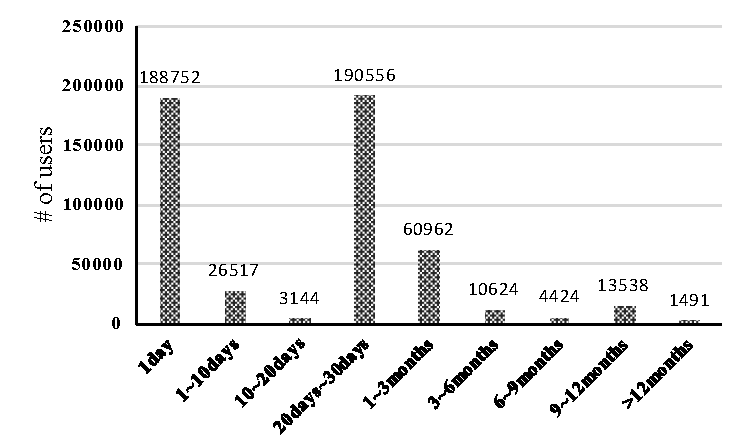
\includegraphics[width=\textwidth]{distribution3.pdf}
  \caption{Real-World Tweeting Situation}
    \floatfoot{The number of users \emph{vs.} the time difference between two
    successive tweets. One can see that the majority of the Twitter
    users tweeted twice between 20 days to 30 days.}
  \label{fig:timediff}
\end{figure}

In the following we present the definitions of the five attribute similarities. For better elaboration, we use $u_1^{t_1}$ and $u_2^{t_2}$ to refer to the two accounts in social network $t_1$ and $t_2$, respectively. 

\noindent \theoremstyle{definition}
\begin{definition}[Location Similarity, $s_1$]
Let $p_{1}^{t_1}$ and $p_{2}^{t_2}$ be the locations set by $u_{1}^{t_1}$ and $u_{2}^{t_2}$, respectively. The location similarity score $s_1$ is defined as
\begin{equation}
s_1(p_{1}^{t_1},p_{2}^{t_2})=
\begin{cases}
1 & if\ p_{1}^{t_1} \mbox{ and } p_{2}^{t_2} \mbox{ are the same},\\
0 & otherwise.
\end{cases}
\end{equation}
\label{def:loc}
\end{definition}
In the social networks we consider, the location in a user's profile follows the format of ``\textit{City, State/Province, Country}'' (a user is not mandatory to fill out all these three fields); a user can also upload the longitude and latitude of his location. In this study, we consider two locations to be the same if (1) cities are the same; or (2) states/provinces are the same; or (3) the Euclidean distance between two coordinates does not exceed 814 miles, which is the approximate diameter of the largest state, Alaska, in the US \cite{alaska}.

\noindent \theoremstyle{definition}
\begin{definition}[Personal Website Link Similarity, $s_2$]
Let $p_{1}^{t_1}$ and $p_{2}^{t_2}$ be the personal website links set by $u_{1}^{t_1}$ and $u_{2}^{t_2}$, respectively. The personal website link similarity score $s_2$ is defined as
\begin{equation}
s_2(p_{1}^{t_1},p_{2}^{t_2})=
\begin{cases}
1 & if\ p_{1}^{t_1}=p_{2}^{t_2},\\
0 & otherwise.
\end{cases}
\end{equation}
\label{def:pw}
\end{definition}
%Here we consider if two personal websites are the same if the links are the same.

\noindent \theoremstyle{definition}
\begin{definition}[Username Similarity, $s_3$]
Let $p_{1}^{t_1}$ and $p_{2}^{t_2}$ be the usernames of $u_{1}^{t_1}$ and $u_{2}^{t_2}$, respectively. The username similarity score $s_3$ is defined as
\begin{equation}
s_3(p_{1}^{t_1}, p_{2}^{t_2})=\frac{|lcs(p_{1}^{t_1},p_{2}^{t_2})|}{\max(|p_{1}^{t_1}|,|p_{2}^{t_2}|)}
\end{equation}
where $lcs(str_1,str_2)$ denotes the \emph{longest common substring} of strings $str_1$ and $str_2$.
\label{def:user}
\end{definition}

\noindent According to the latent semantic analysis (LSA) in NLP \cite{landauer1998introduction}, we defined the biography similarity in the following manner.
\noindent
\begin{definition}[Biography Similarity, $s_4$]
Let $p_{1}^{t_1}$ and $p_{2}^{t_2}$ be the biographies of $u_{1}^{t_1}$ and $u_{2}^{t_2}$, respectively, where $p_{1}^{t_1}$ contains $m_1$ unique words and $p_{2}^{t_2}$ contains $m_2$ unique words. The frequency vector $\vv{fq}(p_{1}^{t_1,4},p_{2}^{t_2})$ is defined as the number of times each word of $p_{1}^{t_1}$ appears in $p_{2}^{t_2}$, i.e., 

$$\vv{fq}(p_{1}^{t_1},p_{2}^{t_2})=\left( 
z_{1},
z_{2},
\cdots,
z_{m_1}
\right)^T$$
with $z_i$ being the number of times the $i$th word of $p_{1}^{t_1}$ appearing in $p_{2}^{t_2}$.
%
Let $F=\vv{fq}(p_{1}^{t_1},p_{2}^{t_2})\cdot \vv{fq}(p_{1}^{t_1},p_{2}^{t_2})^{T}$.  We perform the SVD decomposition against $F$ and retrieve $F$'s singular value vector, which is denoted by $\delta=(\delta_1,\dots,\delta_{m_1})$. Then
the biography similarity $s_4(p_{1}^{t_1},p_{2}^{t_2})$ is defined as
 %
\begin{equation}
\begin{gathered}
s_4(p_{1}^{t_1},p_{2}^{t_2})= \min(\frac{\left\Vert \varSigma\right\Vert _{F}}{\left|p_{1}^{t_1}\right|\left|p_{2}^{t_2}\right|},1)=\min(\frac{\sqrt{\sum_{i=1}^{m}\delta_{m_1}^{2}}}{\sqrt{m_1\cdot m_2}},1)
\end{gathered}
\end{equation}
\label{def:bio}
\end{definition}

\noindent Lastly, due to the special nature of profile images, we consider a profile image with and without human faces separately. %separate the profile images into two types based on whether or not there are human faces in the images.
\noindent
\begin{definition}[Profile Image Similarity, $s_5$]
Let $p_{1}^{t_1}$ and $p_{2}^{t_2}$ be the profile images of $u_{1}^{t_1}$ and $u_{2}^{t_2}$, respectively. The profile image similarity score $s_5$ is defined as:
\begin{equation}
s_5(p_{1}^{t_1}, p_{2}^{t_2})=\begin{cases}
s^F_5(p_{1}^{t_1}, p_{2}^{t_2}), \hbox{both have faces};\\
s^{\neg F}_5(p_{1}^{t_1}, p_{2}^{t_2}), \hbox{none has face};\\
0, \hbox{otherwise}.
\end{cases}
\end{equation}
\label{def:image}
\end{definition}

\noindent For the case when both profile images contain human faces, our approach compares the facial similarity in three steps: (1) \textit{face detection}, (2) \textit{face aligment}, and (3) \textit{face similarity comparison}. In the face dection step, we leverage the Haar Feature-based Cascade Classifier proposed by \cite{viola2001rapid}\cite{lienhart2002extended}; in the face aligment step, we leverage the Multitask Cascaded Convolutional Network proposed and implemented by Zhang \emph{et al.} \cite{zhang2016joint}; and finally, we come up with the face similarity definition motivated by the FaceNet proposed by Schroff \emph{et al.} \cite{schroff2015facenet}. Embedding \cite{schroff2015facenet} is a function $f_{emb}$ whose $L^2$ norm satisfies $\left\Vert f_{emb}(x)\right\Vert _{2}=1$. In our study, we define $f_{emb}$ as
\begin{equation}
f_{emb}(px_{i,j})=\frac{px_{i,j}}{\sqrt{\sum_{i} \sum_{j} px_{i,j}^{2}}}
\end{equation}
where $px_{i,j}$ is the pixel on the $i$-th row and $j$-th colum of an aligned face picture matrix and $d$ is the dimension of the matrix, which is usually two. We define the loss function for the profile images with faces as
\begin{equation}
loss_f=\underset{i,j}{\sum}\left[\left\Vert f_{emb}(px_{i,j}^{p_{1}^{t_1}})-f_{emb}(px_{i,j}^{p_{2}^{t_2}})\right\Vert _{2}^{2}\right]
\end{equation}

\noindent
\begin{customdfn}{5.1}[Profile Image Similarity with Face, $s^{F}_5$]
The face image similarity is defined as
\begin{equation}
s^F_5(p_{1}^{t_1}, p_{2}^{t_2})=\max(1-\sqrt{loss_f}, 0)
\end{equation}
\end{customdfn}

\noindent For the case when both images do not have human faces, we leverage the traditional algorithm, the scale invariant feature transform (SIFT) \cite{lowe1999object}, used for object recognition in computer vision. Let $g(x)$ represent the
number of SIFT features of picture $x$, and $m(x,y)$ be the number of matched features between picture $x$ and $y$ with Lowes's ratio test \cite{lowe2004distinctive}. 
\begin{customdfn}{5.2}[Profile Image Similarity without Face, $s^{\neg F}_5$]
\begin{equation}
\begin{gathered}
s^{\neg F}_5(p_{1}^{t_1}, p_{2}^{t_2}) = \frac{m(p_{1}^{t_1}, p_{2}^{t_2})}{\min(g(p_{1}^{t_1}),g(p_{2}^{t_2})}
\end{gathered}
\end{equation}
\end{customdfn}

Now we are ready to define our overall profile similarity:
\theoremstyle{definition}
\begin{definition}[Profile Similarity]
Let $u_{1}^{t_1}\in SN_1$ and $u_{2}^{t_2}\in SN_2$, the profile similarity $S:SN_1\times SN_2\rightarrow [0,1]$ of two user accounts is defined as
\begin{equation}
S(u_{1}^{t_1},u_{2}^{t_2})=\sum_{k=1}^{5} w_k s_k(p_{1}^{t_1},p_{2}^{t_2})
\label{def:overall}
\end{equation}
where %$p_{1}^{t_1}$ is the $k$-th profile attribute of account $u_{1}^{t_1}$ in the social network $SN_1$, $p_{2}^{t_2}$ is the $k$-th profile attribute of account $u_{2}^{t_2}$ in the social network $SN_2$, 
$s_k(p_{1}^{t_1},p_{2}^{t_2})$ represents the $k$-th attribute similarity of the two user accounts and $w_k$ is the corresponding weight that captures the impact of $s_k$ on the overall profile similarity. 
\end{definition}

In the following we present a learning based model to calculate the weights in Definition~\ref{def:overall}. %, which play a crucial rule for an effective inference. 
%Having specified all the definitions, we need to find the weights for the profile similarity, which are crucial for a correct inference. 
Intuitively, the weights should be determined by maximizing the probability of correct matches and minimizing the probability of incorrect matches. %In order to do so, we employ a learning-based method. 
Suppose we have a ground truth dataset which includes $n_{gt}$ users from $SN_{1}$ and $n_{gt}$ users from $SN_{2}$, with the $i$th user from $SN_{1}$ and the $i$th user from $SN_{2}$ are indeed the same person.
%Suppose we have a ground truth dataset which includes $n_{gt}$ users collected from $SN_{1}=\{u_{1}^{1},u_{1}^{2},\cdots,u_{1}^{n_{gt}}\}$ and $n_{gt}$ users collected from $SN_{2}=\{u_{2}^{1},u_{2}^{2},\cdots,u_{2}^{n_{gt}}\}$ such that each pair of users with the same superscript is indeed the same person. %For example, $u_{1}^{i}$ and $u_{2}^{i}$ from social networks $SN_1$ and $SN_2$ are the same person. 
Based on the profile similarity defined in Definition~\ref{def:overall}, we can get a matrix $\boldsymbol{S}$ over the pairwise profile similarity scores between $SN_{1}$ and $SN_{2}$.
%
\begin{equation}
\mathbf{S}(SN_{1},SN_{2})= \left(\begin{array}{cccc}
S(u_{1}^{1},u_{2}^{1}) & S(u_{1}^{1},u_{2}^{2}) & \ldots & S(u_{1}^{1},u_{2}^{n_{gt}})\\
S(u_{1}^{2},u_{2}^{1}) & S(u_{1}^{2},u_{2}^{2}) & \ldots & S(u_{1}^{2},u_{2}^{n_{gt}})\\
\vdots & \vdots & \ddots & \vdots\\
S(u_{1}^{n_{gt}},u_{2}^{1}) & S(u_{1}^{n_{gt}},u_{2}^{2}) & \ldots & S(u_{1}^{n_{gt}},u_{2}^{n_{gt}})
\end{array}\right)
\end{equation}
where each entry $S(u_{1}^{i}, u_{2}^{j})$ is the profile similarity score defined in Definition~\ref{def:overall}.

In order to find the proper weights, instead of considering only the incorrect matches or correct matches, we came up with a novel loss function which takes into consideration both the correct matches and the incorrect matches, making it more efficient and effective. The loss function is defined as follows:
%
\begin{equation}\label{eq:loss}
\begin{gathered}
loss=l(w_{1},w_{2},\ldots,w_{k})= \\
\left\langle \left[\left(\begin{array}{c}
1\\
1\\
\vdots\\
1
\end{array}\right)_{n_{gt}\times1}-diag(\boldsymbol{S})+\frac{1}{n_{gt}-1}\left(\begin{array}{c}
\underset{j,j\neq1}{\sum}S(u_{1}^{1},u_{2}^{j})\\
\underset{j,j\neq2}{\sum}S(u_{1}^{2},u_{2}^{j})\\
\vdots\\
\underset{j,j\neq n_{gt}}{\sum}S(u_{1}^{n_{gt}},u_{2}^{j})
\end{array}\right)\right]^{2}\right\rangle
\end{gathered}
\end{equation}
where $\left\langle \cdot \right\rangle$ represents the expectation sign. The weight vector is determined by solving the following system of equations.
\begin{equation}\label{eq:gradient}
\nabla l=0\Longrightarrow\begin{cases}
\frac{\partial l}{\partial w_{1}}=0\\
\frac{\partial l}{\partial w_{2}}=0\\
\vdots\\
\frac{\partial l}{\partial w_{k}}=0
\end{cases}
\end{equation}
In our approach, we solve the system of equations (\ref{eq:gradient}) by TensorFlow with the gradient descent optimization \cite{ruder2016overview}.

\subsection{Evaluation}
In this subsection, we report the evaluation results of our approach to demonstrate its effectiveness on the DS-SN attack within a single social network and the SN-SN attack across two social networks.

According to the design elaborated in Section~\ref{sec:dssnapproach}, we implemented the following programs: a malicious app in Java with 3280 lines of code (LOC) for collecting the publicly available Android system state data, which deals with the first step of the DS-SN attack; a server code for activity transition inference and social network event inference with 1800 LOC in Python, which handles the second and third steps of the DS-SN attack; a program of 1595 LOC in Python to crawl the databases of Twitter, Instagram, and Flickr, and perform the device-account matching, which corresponds to the fourth step of the DS-SN attack; and finally, a program with 707 LOC in Python, which performs the SN-SN user account association analysis.

In our experiments, we used five different Android devices: a Nexus 7 with Android version 6.0.1, a HTC One Sense 6 with Android version 5.0.2, a Blu R1 HD with Android version 6.0, a Huawei Honor 8 Lite with Android version 7.0, and a Samsung Galaxy S4 with Android version 4.2.2. In the server side, we used a Dell Inspiron 5559 Specs with Intel Core i7-6500U CPU @ 2.50GHz x 4 running OS Ubuntu 16.04 LTS to conduct the experiments. 

\subsubsection{Effectiveness of the DS-SN Correlation Attack}
We evaluated the effectiveness of our DS-SN attack by i) validating the memory regression learning model, ii) inferring the posting timestamps, iii) inferring the number of characters in a tweet, and iv) inferring the possible list of social network accounts associated with the victim device via multiple posting events.

\textbf{Performance of the Memory Regression Model}

As mentioned in Section~\ref{sec:dssnapproach}, we leveraged a 5-layer feedforward neural network to learn the patterns of activity transitions in Twitter and Instagram, i.e., from \texttt{MainActivity} to \texttt{ComposerActivity} in Twitter and from \texttt{MediaCaptureActivity I} to \\
\texttt{MediaCaptureActivity II} in Instagram. We wrote an automatic program in Python using the Android debug bridge (\texttt{adb})~\cite{adb} with the UI Automator framework for the generation and collection of the training data and test data. We ran the automatic \texttt{adb} Python program in all five Android devices for collecting the training data. As a result, for each of the 5 Android devices, we collected 1,900 pieces of training data for Twitter and 2,340 pieces of training data for Instagram. Thus, in total we have 9,500 pieces of training data for Twitter and 11,700 pieces of training data for Instagram. Note that each piece of the training data contains only the target activity transition - no other noisy actions such as swiping. To determine $n$ as mentioned in Section~\ref{sec:dssnapproach}, we tried multiple different values for the threshold $\delta$ and found that the values around $1000$ work pretty well for both Twitter and Instagram; thus we set $\delta=1000$. Also, we set the cessation threshold for the mean squared error to be $10^{-6}$. As a result, the mean squared error for the learning process of the Twitter activity transition drops to below $10^{-6}$ after approximately 30 minutes and the one for the Instagram activity transition drops to below $10^{-6}$ after approximately 40 minutes, which are reasonably low for deep learning models.

\begin{table*}[t]
\centering
\caption{Averaged Inference Results on the Posting Timestamps and the Number of Characters in Tweeter}
\label{tbl:posttimeinf}
\resizebox{\columnwidth}{!}{
\begin{tabular}{|c|l|c|c|c|}
\hline
\multirow{2}{*}{\begin{tabular}[c]{@{}c@{}}App \\ Name\end{tabular}} & \multicolumn{4}{c|}{Averaged Inference Results on the Posting Timestamps and the Number of Characters in Tweeter}                                                                                                                                                                                                                                                                                                                                                                                                  \\ \cline{2-5}
                                                                     & \multicolumn{1}{c|}{\begin{tabular}[c]{@{}c@{}}Types of \\ Random Noisy \\Actions Performed\end{tabular}} & \begin{tabular}[c]{@{}c@{}}Accuracy of Inferrring\\ Posting Timestamps\end{tabular} & \begin{tabular}[c]{@{}c@{}}Average Difference of\\ Timestamps\\ (in seconds)\end{tabular} &  \begin{tabular}[c]{@{}c@{}}Accuracy of Inferring\\ Number of Characters\\ in Tweets\end{tabular}     \\ \hline
Twitter                                                              & \begin{tabular}[c]{@{}l@{}}1. Swiping\\ 2. Tapping\\ 3. Commenting\\\end{tabular}       & 86.99\%                                                    & 16.35                                                                                                                                            & \multicolumn{1}{l|}{\begin{tabular}[c]{@{}l@{}}37.18\% ($\epsilon=0.05$)\\ 91.86\% ($\epsilon=0.15$)\\ 98.92\% ($\epsilon=0.3$)\end{tabular}}              \\ \hline
Flickr                                                               & \begin{tabular}[c]{@{}l@{}}1. Swiping\\ 2. Tapping\\ 3. Commenting\\\end{tabular}  & 96.81\%                                                    & 15.05                                                                                                                                             & N/A                                                                                                  \\ \hline
Instagram                                                            & \begin{tabular}[c]{@{}l@{}}1. Swiping\\ 2. Tapping\\ 3. Commenting\\\end{tabular}  & 96.73\%                                                    & 19.75                                                                                                                                             & N/A                                                                                                  \\ \hline
\end{tabular}
}
\end{table*}

\textbf{Inference of the Posting Timestamps}

The automatic \texttt{adb} Python program performed 5,625 tests for all five Android devices, with each device performing 1,125 tests. Each test is for one target social network app and collects a block of data with 6 rows: \emph{VSS},  \texttt{tcp\_snd}, and \texttt{tcp\_rcv} for the social network app,  \texttt{utime} and \texttt{stime} for the keyboard process, and \emph{RSS} for the media process, and each row contains 600 values. Therefore, for each Android device, we conducted 375 tests for each target app. It took 5 to 6 minutes to perform one test, during which our automatic \texttt{adb} program controlled the target social network app to tweet with a random number of characters (Twitter) or to post a photo (Instagram and Flickr)), and recorded the system timestamps of the tweet/photo-post event (ground truth timestamps) for evaluation. The \texttt{adb} program also generated random noisy actions such as swiping, tapping, and commenting in the target apps to imitate human beings' actions on these apps during each block collection. %Then in some moments, our program controlled the target apps to tweet with a random number of characters (Twitter) or to post a photo (Instagram and Flickr), and recorded the system timestamp of the tweet/photo-post (ground truth timestamp) for evaluation.
Meanwhile, our malicious app collected \emph{VSS}, \texttt{tcp\_snd}, and \texttt{tcp\_snd} for the three social network apps and the \emph{RSS} of Android media process as shown in Table~\ref{tbl:ds-sn-summary} for the inference attack. 

We considered that a correct inference is made if the difference between the ground truth posting timestamp and our inferred posting timestamp is less than 30 seconds. 
Table~\ref{tbl:posttimeinf} reports the averaged inference results of all Android devices. As one can see, the numbers of correct inferences of the posting timestamps for Twitter, Flickr, and Instagram are 86.99\%, 96.81\%, and 96.73\%, respectively. Table~\ref{tbl:eachdeviceinfer} shows the inference results of each Android device against the three target apps. As one can see, generally speaking, our inference of posting timestamps is most effective in Nexus 7 device, and least effective in HTC One Sense 6.

Note that in our memory regression model we set $\sigma=10^5$, which was determined based on many trials. 

\begin{table}[]
\centering
\caption{Inference Results on the Posting Timestamps for Each Device}
\label{tbl:eachdeviceinfer}
\begin{tabular}{|c|c|c|c|}
\hline
\multirow{2}{*}{Device Name} & \multicolumn{3}{c|}{App Name} \\ \cline{2-4} 
                             & Twitter & Instagram & Flickr  \\ \hline
Nexus 7                      & 90.67\% & 98.67\%   & 99.73\% \\ \hline
HTC One Sense 6              & 82.93\% & 91.20\%   & 90.40\% \\ \hline
Blu R1 HD                    & 91.47\% & 87.47\%   & 98.67\% \\ \hline
Huawei Honor 8               & 84.27\% & 94.93\%   & 98.40\% \\ \hline
Samsung Galaxy S4            & 90.93\% & 85.87\%   & 98.93\% \\ \hline
\end{tabular}
\end{table}


\begin{table*}[!htb]
\centering
\caption{Attack Results on Volunteers}
\label{tbl:volunteers}
\resizebox{1.2\columnwidth}{!}{
\hspace{-27ex}
\begin{tabular}{|c|c|c|c|c|c|c|c|c|c|c|c|c|}
\hline \hline
\multicolumn{13}{|c|}{Attack Results on Volunteers}                                                                                                                                                                                                                                                                                                                                                                                                                                                                                                                                                                                                                                                                     \\ \hline \hline
\multirow{2}{*}{\# of Timestamps} & \multicolumn{6}{c|}{\begin{tabular}[c]{@{}c@{}}Number of Potential \\ Twitter Identities\\ (Without Number-of-Character Filter)\end{tabular}} & \multicolumn{6}{c|}{\begin{tabular}[c]{@{}c@{}}Number of Potential \\ Twitter Identities\\ (With Number-of-Character Filter)\end{tabular}}                                                                                                                                                                                                                                                                                                                                                                                              \\ \cline{2-13} 
                                  & Participant 1          & Participant 2          & Participant 3          & Participant 4          & Participant 5          & Average          & Participant 1                                                                        & Participant 2                                                                        & Participant 3                                                                        & Participant 4                                                                        & Participant 5                                                                        & Average                                                                              \\ \hline
1                                 & 52,120                 & 61,810                 & 55,132                 & 51,205                 & 50,037                 & 54,060           & \begin{tabular}[c]{@{}c@{}}2,313 ($\epsilon=0.3$)\end{tabular} & \begin{tabular}[c]{@{}c@{}}2,538 ($\epsilon=0.3$)\end{tabular} & \begin{tabular}[c]{@{}c@{}}2,272 ($\epsilon=0.3$)\end{tabular} & \begin{tabular}[c]{@{}c@{}}1,971 ($\epsilon=0.3$)\end{tabular} & \begin{tabular}[c]{@{}c@{}}2,067 ($\epsilon=0.3$)\end{tabular} & \begin{tabular}[c]{@{}c@{}}2,232 ($\epsilon=0.3$)\end{tabular} \\ \hline
2                                 & 369                    & 403                    & 331                    & 324                    & 347                    & 354              & \begin{tabular}[c]{@{}c@{}}21 ($\epsilon=0.3$)\end{tabular}       & \begin{tabular}[c]{@{}c@{}}19 ($\epsilon=0.3$)\end{tabular}       & \begin{tabular}[c]{@{}c@{}}22 ($\epsilon=0.3$)\end{tabular}       & \begin{tabular}[c]{@{}c@{}}12 ($\epsilon=0.3$)\end{tabular}       & \begin{tabular}[c]{@{}c@{}}10 ($\epsilon=0.3$)\end{tabular}       & \begin{tabular}[c]{@{}c@{}}16 ($\epsilon=0.3$)\end{tabular}       \\ \hline
3                                 & 52                     & 61                     & 71                     & 43                     & 57                     & 56               & \begin{tabular}[c]{@{}c@{}}1 ($\epsilon=0.3$)\end{tabular}         & \begin{tabular}[c]{@{}c@{}}1 ($\epsilon=0.3$)\end{tabular}         & \begin{tabular}[c]{@{}c@{}}2 ($\epsilon=0.3$)\end{tabular}         & \begin{tabular}[c]{@{}c@{}}1 ($\epsilon=0.3$)\end{tabular}         & \begin{tabular}[c]{@{}c@{}}1 ($\epsilon=0.3$)\end{tabular}         & \begin{tabular}[c]{@{}c@{}}1 ($\epsilon=0.3$)\end{tabular}         \\ \hline
4                                 & 11                     & 8                      & 13                     & 9                      & 7                      & 9                & \begin{tabular}[c]{@{}c@{}}1 ($\epsilon=0.3$)\end{tabular}         & \begin{tabular}[c]{@{}c@{}}1 ($\epsilon=0.3$)\end{tabular}         & \begin{tabular}[c]{@{}c@{}}1 ($\epsilon=0.3$) \end{tabular}         & \begin{tabular}[c]{@{}c@{}}1 ($\epsilon=0.3$)\end{tabular}         & \begin{tabular}[c]{@{}c@{}}1 ($\epsilon=0.3$)\end{tabular}         & \begin{tabular}[c]{@{}c@{}}1 ($\epsilon=0.3$)\end{tabular}         \\ \hline
5                                 & 4                      & 3                      & 5                      & 4                      & 3                      & 3                & \begin{tabular}[c]{@{}c@{}}1 ($\epsilon=0.3$)\end{tabular}         & \begin{tabular}[c]{@{}c@{}}1 ($\epsilon=0.3$)\end{tabular}         & \begin{tabular}[c]{@{}c@{}}1 ($\epsilon=0.3$)\end{tabular}         & \begin{tabular}[c]{@{}c@{}}1 ($\epsilon=0.3$)\end{tabular}         & \begin{tabular}[c]{@{}c@{}}1 ($\epsilon=0.3$)\end{tabular}         & \begin{tabular}[c]{@{}c@{}}1 ($\epsilon=0.3$)\end{tabular}         \\ \hline
6                                 & 3                      & 2                      & 2                      & 1                      & 1                      & 1                & \begin{tabular}[c]{@{}c@{}}1 ($\epsilon=0.3$)\end{tabular}         & \begin{tabular}[c]{@{}c@{}}1 ($\epsilon=0.3$)\end{tabular}         & \begin{tabular}[c]{@{}c@{}}1 ($\epsilon=0.3$)\end{tabular}         & \begin{tabular}[c]{@{}c@{}}1 ($\epsilon=0.3$)\end{tabular}         & \begin{tabular}[c]{@{}c@{}}1 ($\epsilon=0.3$))\end{tabular}         & \begin{tabular}[c]{@{}c@{}}1 ($\epsilon=0.3$)\end{tabular}         \\ \hline
7                                 & 3                      & 2                      & 1                      & 1                      & 1                      & 1                & \begin{tabular}[c]{@{}c@{}}1 ($\epsilon=0.3$)\end{tabular}         & \begin{tabular}[c]{@{}c@{}}1 ($\epsilon=0.3$)\end{tabular}         & \begin{tabular}[c]{@{}c@{}}1 ($\epsilon=0.3$)\end{tabular}         & \begin{tabular}[c]{@{}c@{}}1 ($\epsilon=0.3$)\end{tabular}         & \begin{tabular}[c]{@{}c@{}}1 ($\epsilon=0.3$)\end{tabular}         & \begin{tabular}[c]{@{}c@{}}1 ($\epsilon=0.3$)\end{tabular}         \\ \hline
8                                 & 1                      & 2                      & 1                      & 1                      & 1                      & 1                & \begin{tabular}[c]{@{}c@{}}1 ($\epsilon=0.3$)\end{tabular}         & \begin{tabular}[c]{@{}c@{}}1 ($\epsilon=0.3$)\end{tabular}         & \begin{tabular}[c]{@{}c@{}}1 ($\epsilon=0.3$)\end{tabular}         & \begin{tabular}[c]{@{}c@{}}1 ($\epsilon=0.3$)\end{tabular}         & \begin{tabular}[c]{@{}c@{}}1 ($\epsilon=0.3$)\end{tabular}         & \begin{tabular}[c]{@{}c@{}}1 ($\epsilon=0.3$)\end{tabular}         \\ \hline
9                                 & 1                      & 1                      & 1                      & 1                      & 1                      & 1                & \begin{tabular}[c]{@{}c@{}}1 ($\epsilon=0.3$)\end{tabular}         & \begin{tabular}[c]{@{}c@{}}1 ($\epsilon=0.3$)\end{tabular}         & \begin{tabular}[c]{@{}c@{}}1 ($\epsilon=0.3$)\end{tabular}         & \begin{tabular}[c]{@{}c@{}}1 ($\epsilon=0.3$)\end{tabular}         & \begin{tabular}[c]{@{}c@{}}1 ($\epsilon=0.3$)\end{tabular}         & \begin{tabular}[c]{@{}c@{}}1 ($\epsilon=0.3$)\end{tabular}         \\ \hline
\end{tabular}
}
\end{table*}

\textbf{Inference of the Number of Characters in a Tweet}

To evaluate the inference accuracy on the number of characters in a tweet through CPU \texttt{utime} and \texttt{stime} of the Keyboard process, we denote the actual number of characters of a tweet by $N_{act}$, the inferred number by $N_{inf}$, and set an error parameter $\epsilon$ such that our inference is considered a success if the error percentage is less than $\epsilon$, i.e., $\frac{|N_{act}-N_{inf}|}{N_{act}}\le\epsilon$. 
In order to evaluate the accuracy of our inference attacks, we randomly sampled 5,000 tweets from those of the 500,008 Twitter users collected in Section~\ref{sec:dssnapproach}, and re-tweeted these 5,000 tweets using our Android devices. By doing so, we can guarantee that the distribution of the number of characters of our posted tweets follows the one in real-world.
The average number of characters of these 5,000 tweets was 189. The results are reported in Table~\ref{tbl:posttimeinf}, which indicate that if we set $\epsilon$ to be 0.05, the possibility of correct inference is 37.18\%; if $\epsilon$ is set to 0.15, the possibility of correct inference is 91.86\%; while if $\epsilon$ is set to 0.3, the possibility increases to 98.92\%. %Table~\ref{tbl:posttimeinf} shows the detailed results. 

\textbf{Associating Device with Social Network Accounts}

We used Twitter to illustrate the performance of associating the victim device with a list of candidate social network accounts. In this evaluation, we conducted two studies, with one on the Twitter celebrities and one on five volunteers. Note that the study on Twitter celebrities cannot identify any device that is associated with a social network account because we do not install our malicious app in any legitimate user in Twitter; nevertheless, the tweeting activities of celebrities can facilitate us to figure out how many people simultaneously tweet at two or more timestamps, which provides a perfect justification to explain why we can correlate the tweeting activities at different timestamps to identify the user account associated with a victim device.

For the study on celebrities, we collected tweets from 5 active Twitter celebrities, with 10 tweets for each at different timestamps, from November 2016 to February 2017, to get the data at 50 different timestamps. Each celebrity has at least 20 million followers. We considered celebrities as our study subjects because they not only use real identities, but also are active on Twitter. The results are reported in Table~\ref{tbl:celeb-eval}, which indicate that the average number of Twitter users who tweeted at one timestamp is 52,016, at the same two timestamps is 359, at the same three timestamps is 61, and at the same four timestamps is 6. These results are interesting as one can see that the number of users who tweeted simultaneously at multiple timestamps drops significantly as the number of considered timestamps increases. 

\begin{table}[t]
\centering
\caption{Attack Results on Celebrities}
\label{tbl:celeb-eval}
\small
\begin{tabular}{|c|c|}
\hline \hline
\multicolumn{2}{|c|}{Attack Results on Celebrities}                                              \\ \hline \hline
\# of Timestamps & \begin{tabular}[c]{@{}c@{}}Average Number of \\ Potential Twitter Identities\end{tabular} \\ \hline
1                & 52,016                                                                                    \\ \hline
2                & 359                                                                                       \\ \hline
3                & 61                                                                                        \\ \hline
4                & 6                                                                                         \\ \hline
\end{tabular}
\end{table}

Besides using celebrities as testing subjects mentioned above, we also recruited five volunteers to participate in our evaluation process. Each participant used one of our five Android devices to tweet 10 times at 10 different timestamps with his/her own Twitter account. Each tweet contained a random number of characters. The detailed results are shown in Table~\ref{tbl:volunteers}. If we do not apply the number of tweeted characters as a filter, we found that in average there are 54,060 users who tweeted at one timestamp as the volunteers did. Then the number goes to 354 at two same timestamps, 56 at three same timestamps, 9 at four same timestamps, 3 at five same timestamps, and 1 at six same timestamps. These numbers indicate that an attacker needs to conduct the inference attack for an average of six times in order to associate the Twitter account of one of our voluteers with his/her device without applying the number of characters as a filter. If we apply this filter, as one can see from the results, an attacker only needs to conduct the inference attack for an average of three times to successfully associate one volunteer with his/her Twitter account. 

\subsubsection{Performance of the SN-SN Correlation Attack}
As one can see from the results shown above, an attacker needs to infer at least three timestamps on average to correlate a user's social network account with his/her device with the estimated number of characters as a filer. Without applying this filter, on average at least 6 timestamps need to be inferred. To speed up this process, SN-SN correlation attack can be launched. In this subsection, we evaluate the performance of the SN-SN correlation attack.

Since Instagram does not provide an interface via which we can retrieve posts at any given timestamp, we considered the other two social networks: Twitter and Flickr. To proceed, we need to first derive the weight for each attribute in order to calculate the profile similarity. For this purpose we need ground truth data to train our learning model proposed in Section~\ref{sec:snsnattack}. We manually checked the tweets of a large amount of Twitter users and filtered out those who do not explicitly provide their Flickr links in one of their tweets. Finally, we obtained 20 pairs of Twitter and Flickr users we were certain that each pair actually refers to the same person. Then we applied these data to minimize the loss function in equation \eqref{eq:loss}. Finally, we obtained the following weights when the loss function reaches its stationary minimum of 0.108886: $\omega_{1}=0.509717$, $\omega_{2}=0.194603$, $\omega_{3}=0.51427$, $\omega_{4}=0.171117$ and $\omega_{5}=0.30354$. Lastly, we normalized these weights by setting $\omega_{i}^*=\frac{\omega_{i}}{|\sum_{i=1}^{5}\omega_i|}$, and obtained $\omega_{1}^*=0.301029$, $\omega_{2}^*=0.114929$, $\omega_{3}^*=0.303718$, $\omega_{4}^*=0.101058$, and $\omega_{5}^*=0.179265$.

As one can see from the above, username ($\omega_{3}$) plays an extremely important role in determining whether two users from two different social networks are actually the same person, followed by location ($\omega_{1}$).  The least important factor is biography ($\omega_{4}$), which indicates that people tend to write differently for different social networks.

\begin{figure}[t]
  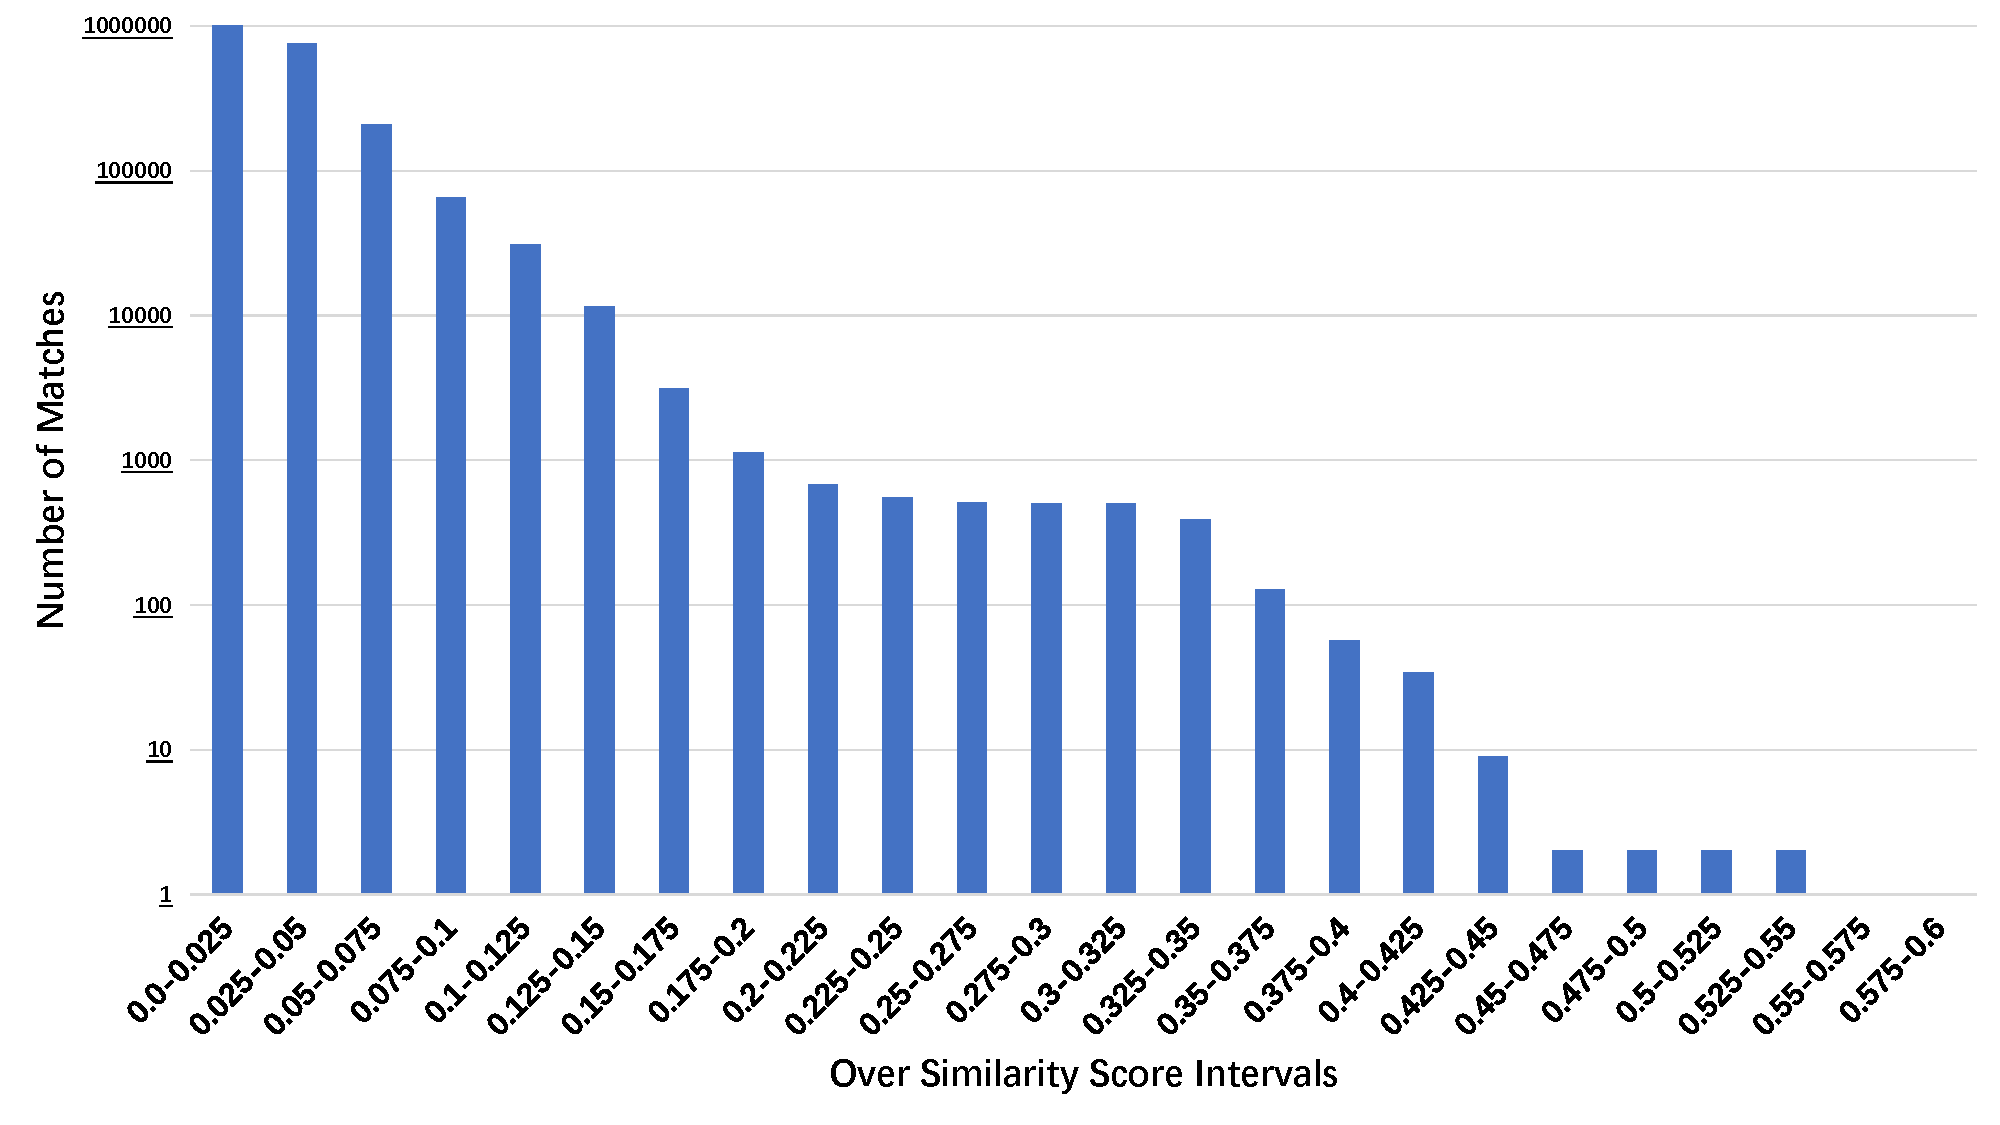
\includegraphics[width=\textwidth]{SN-SN-match.pdf}
  \caption{Distribution of the Matches}
  \floatfoot{The distribution of the matches of the fifth participant. The x-axis is the intervals of overall similarity scores while the y-axis is the number of matches.}
  \label{fig:sn-sn-match}
\end{figure}

Next we analyzed the Twitter-Flickr matching performance. We asked each of the five volunteers to send a post in Flickr with his/her Flickr account after he/she finished the 10 tweeting experiments mentioned above. Then we correlated Flickr with Twitter by considering only the first timestamp of the Twitter data of all the participants. % shown in table~\ref{tbl:volunteers} by applying an number-of-character filter of $\epsilon=0.3$. 
Next we crawled all the posts in Flickr at the five timestamps corresponding to those at which our five participants sent posts. As a result, we found that there were totally 611 Flickr users who also posted at the same timestamp at which the first participant posted. The numbers of Flickr users who posted at the same time as the second, third, fourth, and fifth participant were 533, 421, 498, and 506, respectively. Therefore, for the first participant, we analyzed a similarity matrix $\boldsymbol{S}_{p_1}$ defined in Section~\ref{sec:dssnapproach} with 1,413,243 entries ($2,313\times 611$). Similarly, the numbers of entries in the similarity matrices for the second, third, fourth, and fifth participant were 1,352,754 ($2,538\times 533$), 956,521 ($2,272\times 421$), 945,204 ($1,898\times 498$), and 1,112,188 ($2,198\times 506$), respectively. Ideally, the majority of the entries in these five matrices should contain very small values,  i.e., close to zero; while the entries for the  correct matches contain big values, i.e., close to one.

After we evaluated the five matrices with the trained weights obtained above, the similarity matrix of the first participant shows that 1,332,575 entries (94.29\%) are below 0.1; only 3 pairs whose similarity scores are greater than 0.5; and only 1 pair whose similarity score is greater than 0.65, which is the correct matching, i.e., the Twitter account and the Flickr account of the first participant. Similarly, our results showed that over 90\% of all the entries of the similarity matrices of the other four participants are below 0.1; and the correct matches corresponds to the  pairs with the highest scores. Among the results of all the five participants, the highest overall similarity score is the one for the fifth participant, which is 0.84. Figure~\ref{fig:sn-sn-match} illustrates the detailed distribution of the matches of the fifth participant as an example.
These results not only indicate that both our definitions of the attribute similarities and the weights work well in real cases, but also imply that our SN-SN correlation attack is effective in facilitating the DS-SN attack to speed up the device-identity association attack.

\subsection{Related Works}
\label{sec:related}

In this subsection, we summarize the most related work from two aspects: side-channel attacks in mobile systems and privacy attacks in social networks.

\noindent\textbf{Side-channel Attacks in Mobile Systems}. Side-channel attacks in mobile systems have been causing more and more concerns in recent years. Chen \emph{et al.} \cite{chen2014peeking} managed to infer the UI state and deploy multiple attacks based on the side-channel information such as memory, CPU, and network statistical data stealthily obtained by a zero-permission malicious app residing in the victim's smartphone. Li \emph{et al.} \cite{li2016csi} proposed a keystroke inference attack targeting mobile devices by performing the principal component analysis (PCA) on the channel state information that could be affected by the finger motions through a public WiFi hotspot. 
Zhou \emph{et al.} \cite{zhou2013identity} exploited the side-channel information of Android devices to infer a user's private information, e.g., rough location, health condition, investment, and driving route. Yang \emph{et al.}  \cite{yang2016inferring} presented an approach to discover which website a user is browsing by analyzing the USB power while the smartphone is charging. Song \emph{et al.} \cite{song2016my} managed to crack a 3D printer by reconstructing the physical prints and their corresponding G-code through scrutinizing acoustic and magnetic information obtained from Android built-in sensors. Gruss \emph{et al.} \cite{gruss2016prefetch} exploited the prefetch instructions to defeat address space layout randomization (ASLR), which is a technique to make the memory address unpredictable for an attacker to launch code-reuse attacks such as return-oriented programming (ROP). Van \emph{et al.} \cite{van2016drammer} took a step further to attack hardware by launching a row hammer attack and using timing inference to make the row hammer attack deterministic compared to prior attacks which can only succeed on a probabilistic sense. Li \emph{et al.} \cite{li2016side} proposed a side-channel attack to infer the basic living activities by analyzing the changes of the traffic sizes of encrypted video streams in smart home surveillance.
Yang \emph{et al.} \cite{yang2018study} identified and systematically analyzed a new security issue in HTML5-based hybrid mobile applications, which is termed the Origin Stripping Vulnerability (OSV), and proposed an OSV detection mechanism, namely OSV-Hunter, which leverages the \texttt{postMessage} API to defend against OSV from the root. 
Zhang \emph{et al.} \cite{zhang2018empirical} conducted an empirical study on the problem of cross-principal manipulation (XPM) of web resources, and designed a toll named XPMChecker to automatically detect XPM. An analysis generated by XPMChecker reveals that nearly 49.2\% apps from Google Play were affected by the XPM issue \cite{zhang2018empirical}.
Side-channel information is now an essential ingredient of the mobile system security.

%\noindent\textbf{Security and Privacy of Smart Device}. The security and privacy of smart devices are causing more and more concerns. %The most relevant works are aforementioned as our motivating examples. 
%Zhou \emph{et al.} \cite{zhou2013identity} managed to exploit the side-channel information of Android devices in order to infer the user's private information, e.g., rough location, health condition, investment, and driving route. Chen \emph{et al.} \cite{chen2014peeking} leveraged a Hidden Markov Model (HMM) to infer which landing \texttt{Activity}/UI a user currently resides and managed to implement serious attacks such as UI phishing and camera peeking, which could potentially result in devastating consequences. Besides these two works, side-channel based inference attacks remain a hot topic in recent years. Yang \emph{et al.}  \cite{yang2016inferring} managed to discover which website a user is browsing through analyzing the USB power while the smartphone is charging. Song \emph{et al.} \cite{song2016my} managed to crack the 3D printer by reconstructing the physical prints and their corresponding G-code through scrutinizing acoustic and magnetic information which can be obtained from Android built-in sensors. Gruss \emph{et al.} \cite{gruss2016prefetch} exploited the prefetch instructions to defeat address space layout randomization (ASLR), which is the technique to make the memory address unpredictable for an attacker to launch code-reuse attacks such as return-oriented programming (ROP). Van \emph{et al.} \cite{van2016drammer} even took a step forward to attack the hardware by launching row hammer attack and using timing inference to make the row hammer attack deterministic compared to prior attacks which can only succeed on a probabilistic sense. This attack results in rooting an Android device without exploiting any software vulnerability. Timing attack is also a serious threat to user privacy. Stone \emph{et al.} \cite{stone2013pixel} systematically analyzed web browser based timing attack such as CSS shader with WebGL and managed to sniff user browsing history and to steal pixels. Jia \emph{et al.} \cite{jia2015know} managed to accurately infer the exact residential location of a user by exploiting browser cache queries. % performing timing attack which exploits browser cache queries.

\noindent\textbf{Social Network Privacy}. Studies showed that privacy of social networks can be breached in multiple ways. Backes \emph{et al.} \cite{backes2017identity} proposed a novel link prediction inference attack between any pair of individuals in social networks based on their mobility profiles. Wondracek \emph{et al.} \cite{wondracek2010practical} demonstrated that it is possible to de-anonymize a user on a social network through his membership in specific social network groups by exploiting the browser cache in order to detect whether a user has visited certain URLs of a group. Nilizadeh \emph{et al.} \cite{nilizadeh2014community} proposed a community-based large scale de-anonymization attack using structural similarity. Ji \emph{et al.} \cite{Ji2015OnYS} presented the seed quantification requirements for perfect de-anonymizability and partial de-anonymizability of real-world social networks, which consolidate the de-anonymization at theory level. Srivatsa \emph{et al.} \cite{srivatsa2012deanonymizing}, on the other hand, leveraged mobility traces with social networks as side-channel information to uncover users' real identities. Lai \emph{et al.} \cite{lai2015anonymizing} exploited a user's interest group information to de-anonymize the users on social networks. Existing studies % not only focused on uncovering identities for social network users but also tended to reveal hidden attributes for social network users. 
also tended to reveal hidden attributes for social network users. Chaabane \emph{et al.} \cite{chaabane2012you} exploited a user's interest to explore hidden attributes of a user, e.g., age, gender, and so on. Mei \emph{et al.} \cite{Mei2018TNSE} reported an inference attack framework that integrates and modifies the existing state-of-the-art convolutional neural network models to infer a user's age. Gong \emph{et al.} \cite{gong2016you} proposed a new type of inference against user's hidden attributes such as location, occupation, and interest by analyzing both his social friending and behavioral records. 
Hassan \emph{et al.} \cite{hassan2018analysis} analyzed the privacy threats in fitness-tracking social networks and developed an attack against Endpoint Privacy Zones (EPZs) to extract a user's sensitive locations. They also presented an EPZ fuzzing technique based on geo-indistinguishability to mitigate a user's privacy leak through fitness-tracking social networks.
Many of these attacks mainly de-anonymize users based on their social relationships in a large dataset, while our approach can precisely identify the social network accounts of a target user behind a device based on the device's side-channel information, the public social network events, and the profile similarity of the user's accounts in different social networks.


   \newpage
   \begin{singlespace}
   \section{CLAF: A Credential-Less Authentication Framework for Smart Home Systems}
   \end{singlespace}
   \label{sec:claf}
   
\subsection{Threat Models}
Considering the two security problems, we formulate the following four threat models that basically cover all kinds of practical attacks an adversary can launch against a smart home system. In Section~\ref{subsec:claf-eval}, we detail the implementation of at least one attack for each threat model, to demonstrate how our proposed CLAF framework can protect the smart home systems from being severely affected by the two security problem. 

\begin{itemize}
\item An attacker penetrates a victim's LAN and controls the smart home system within the LAN. 
For example, the attacker can penetrate a victim's LAN by creating a malicious website and control a user's smart home devices without using any malicious payload~\cite{jia2018traffic}. 

\item An attacker spoofs itself as a trusted source, i.e., a smart home app or a smart home server. For example, the attacker can spoof the IP address of a legitimate user's smart home app.  
IP spoofing is a mature and practical tool that has been widely adopted by attackers in industry~\cite{tanase2003ip}. 

\item An attacker compromises a victim's smartphone at a shallow level. For example, the victim can be lured to install a malicious app that runs on his smartphone to control his smart home devices. Obviously, this threat model can be exploited by overprivileged apps to carry out various attacks. 
360 security lab and MWR lab respectively demonstrated that it is feasible to covertly install a malicious app on iPhone 7 and Samsung Galaxy S8 by luring a user to visit a malicious website~\cite{pwn2own2017}. 

\item An attacker compromises a victim's smartphone at a deeper level. For example, the attacker can lure the victim to connect his smartphone to the attacker's malicious equipment via USB. %since USB access is always granted with higher permission such as 

\end{itemize}

Note that we do not consider the case in which an attacker physically trespasses a victim's home or physically accesses the victim's devices; nor do we consider the case where an attacker is able to compromise any user's device to the kernel level such as rooting the user's smartphone or gain the system privilege of any device, since compromising a device to the kernel level requires a great amount of effort and it also makes all security measures meaningless.

\subsection{Approach Overview}
\label{subsec:claf-approach}
In this section, we first describe a general smart home system model under our consideration. Then we present CLAF, a Credential-Less Authentication Framework, to protect the smart home systems from being affected by the unavoidable open-port and overprivilege problems. Finally, we detail the design of CLAF, give examples to demonstrate how CLAF plays its role, and compare CLAF with the two recently proposed mechanisms defending against the overprivilege problem of smart home systems. 

\subsubsection{A General Smart Home System Model}
A typical smart home system contains smart home devices, a router, a central hub (optional), one or more smartphones serving as controllers, smart home apps running on the smartphones, and smart home servers.  %is the most important device for handling all the network traffics, 
The router handles all network traffics, and all operations eventually need to go through it in order to reach the target smart home devices. The devices supporting Wi-Fi are directly connected to the router. The central hub, if available, serves as a gateway through which smart home devices that do not have the Wi-Fi interface are connected to the router. Smart home apps provide interfaces for the users to generate and send operations, e.g., turning on/off lights and locking the door. Each smart home device has a corresponding app running on the smartphone controllers through which a user or the smartphones can conveniently interact with the device. All operations controlling the physical smart home devices must be issued by the apps running on the smartphones.  The apps hosted by the smartphones act jointly based on the states of the home measured by the deployed smart devices to realize home automation. For example, the room temperature measured by a smart thermostat can trigger an AV app to turn on the air conditioning system when the temperature is higher than $80^\circ$F at daytime. Note that how to realize home automation based on the sensing data is out of the scope of this paper as we mainly focus on preventive measures against the two challenging security problems. The operations can either be sent to the smart home servers which then forward them to the router, or be sent to the router directly. The router delivers the operations to the directly connected target smart home devices, or via the central hub which converts the incoming traffic based on the specific outgoing communication interface such as Zigbee or Bluetooth to reach the target device. The overall system architecture is shown in Figure~\ref{fig:system}. A few popular smart home systems such as Samsung~\cite{samsungsmarthome}\footnote{The Samsung smart home system can also employ the SmartThings server working as controller to host all smart device apps but here we consider the Samsung system that adopts smartphones as controllers to host all smart device apps.} and Xiaomi~\cite{xiaomismarthome} adopt this architecture with a central hub while others such as systems of Amazon Alexa, Google Home, Wink, Caster, TP-LINK, and Belkin support the architecture without a central hub~\cite{bestselling}.


\begin{figure}[!htb]
        \centering
        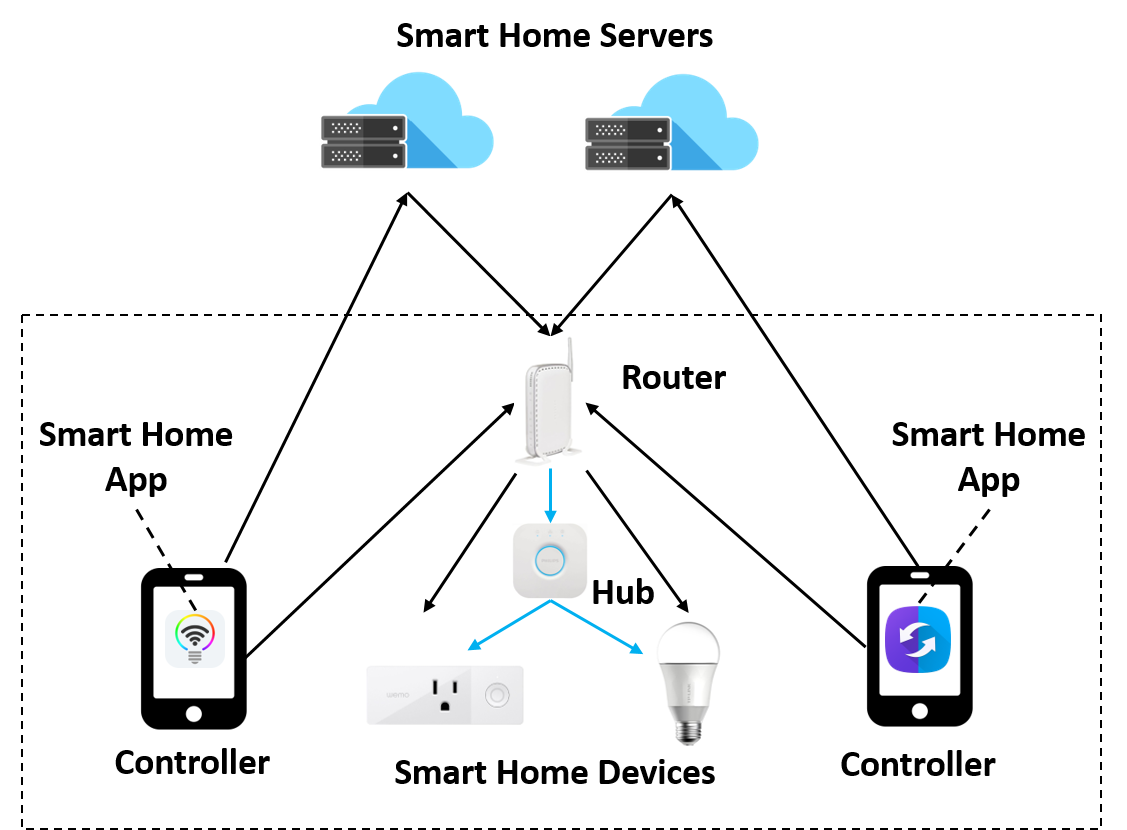
\includegraphics[scale=0.3]{system.png}
        \caption{A general Smart Home System Model}
        \label{fig:system}
\end{figure}




\subsubsection{The CLAF Framework} \label{sec:CLAF:Framework}

We propose CLAF, a Credential-Less Authentication Framework, aiming at providing a cage to regulate the activities of an overprivileged app and control the access to a device with ports open to the public. CLAF satisfies the following design objectives:
\begin{itemize}
\item with CLAF, an overprivileged app should not be able to perform any operation it is not supposed/allowed to;
\item with CLAF, an open port should not be able to accept any operation given by an unauthorized user/device;
\item with CLAF, no modification or patching to the firmware/hardware of the current smart home devices is needed;
\item CLAF should be light-weight, extensible, and flexible for versatile smart home configurations. 
\end{itemize}

CLAF contains three major components: \emph{an evidence provider}, \emph{an operation handler}, and \emph{a policy server}. The operation handler maintains a policy cache storing a copy of the policies maintained by the policy server. An \textit{evidence} provides a credential-less proof of an operation which is an action launched to control or access a smart home device; and a \textit{policy} serves as a permission manager indicating whether an operation from a certain smart home app should be permitted. They are formally defined as follows.

\begin{definition}[\textit{Evidence}]\label{def:evidence}
An \textit{evidence} $e$ of an operation $op$ is a 4-tuple $e=(id, op, h, t)$, where $id$ is the identity of the smart home app who launches the operation $op$; $h$ indicates how the $op$ is launched, e.g., whether user interaction is involved; and $t$ is the time when the $op$ is launched. It answers the question of ``\textit{who did what at when by how}''. For example, an evidence \emph{(smart door app, opening the door, human interaction, current time)} indicates that a door-open command is just issued by the user via the smart door lock/unlock app. 
\end{definition}

\begin{definition}[\textit{Policy}]\label{def:policy}
A \textit{policy} $p$ is a 3-tuple $p =(id, op, h)$, where $id$ is the identity of the smart home app who launches the operation $op$ and $h$ indicates how the $op$ is launched. It answers the question of ``\emph{who can do what by how}''. For example, a policy \emph{(smart coffee machine app, making coffee, human interaction)} indicates that the smart coffee machine can make a cup of coffee when a command is issued by a human being via the corresponding app; an operation of opening the window  issued by the coffee machine app will be blocked as there exists no such a policy in the policy cache/server.
\end{definition}

An \textit{evidence} can be collected and then forwarded to the operation handler to prove that the operation is a legitimate one. It serves as a wall to prevent the operations issued by outsiders that exploit the open-ports from being passed to the smart home system: no evidence can be sent to the operation handler if the operation is not issued by a legitimate app hosted by the smartphone controller.
A \textit{policy} must be user-defined and pre-stored in the policy server. These \textit{policies} may be updated under three situations: (1) when a new device is added into the system; (2) when a firmware of a device is updated; and (3) a legitimate user wishes to modify them (e.g., adding or removing operations supported by an app). Such a flexible user-defined policy mechanism can successfully prevent the operations issued by overprivileged apps. Note that we require certain operations such as \emph{opening the garage door} or \emph{turning on the oven} should only be launched by human beings pushing a button through the corresponding app as they may bring higher security risks, while others such as \emph{turning on the air conditioning system when the room temperature is above $80^\circ$F} can be automatically issued by a smart AV app (without human interaction). 
%\emph{opening the windows when the room temperature is above $80^\circ$F} can be automatically issued by a smart window app at daytime while human interaction must be involved at bedtime. 

Considering the general smart home system architecture presented in Figure~\ref{fig:system}, one can see that it is reasonable for the evidence provider to be operated on the user's smartphone for collecting and sending \textit{evidences} to the operation handler, the operation handler to be operated on the router in charge of passing and filtering operations based on the \textit{policies}, and the policy server to be operated on a secure cloud server (smart home server) storing the user-defined \textit{policies} and synchronizing them with the policy cache residing in the operation handler when the \textit{policies} are updated. All operations are generated by the apps in the smartphone, and the smartphone learns the home states based on the data collected by the smart devices, based on which to trigger the corresponding apps to act. We assume that the communications between the evidence provider and the operation handler, and all communications involving the policy server, are secure and tamper-resistant. This can be simply realized by applying SSL/TLS and certificate verification, as the smartphone, router, and server hosting the three CLAF components possess sufficiently strong computational capabilities.  We further assume that the smartphone, router, and server are (loosely) time-synchronized. 

Intuitively one can ask the evidence provider to collect evidence and send it to the operation handler when the operation is launched by a device app. However, this needs to make modifications to the device app such that it can trigger the evidence provider to collect evidence when an operation is launched, which is not practical when the app is not an open source one. This leaves us a tedious way to overcome the challenge: one can ask the evidence provider to continuously collect  and analyze evidence, and send it to the operation handler when an operation is detected from the evidence. This approach may work but it places a heavy burden on the smartphone controller. Alternatively, one can ask the operation handler to send a request to the evidence provider whenever an operation is received, which is lightweight and practical as smart home operations that command the smart devices are not frequent. In our implementation, we take the second approach, which requires the operation handler to communicate with the evidence provider asking for an evidence when an operation is received. 

If a fresh \textit{evidence} is available, whether obtained with the operation or requested independently, the operation handler checks the evidence content ($id$, $op$, $h$) against the user-defined policies stored in the policy cache, and let the operation proceed only if there exists a policy entry with perfectly matched $id$, $op$, and $h$. If no evidence is received for an operation within a small time interval, the operation is blocked. 

\begin{figure*}[!htb]
        \centering
        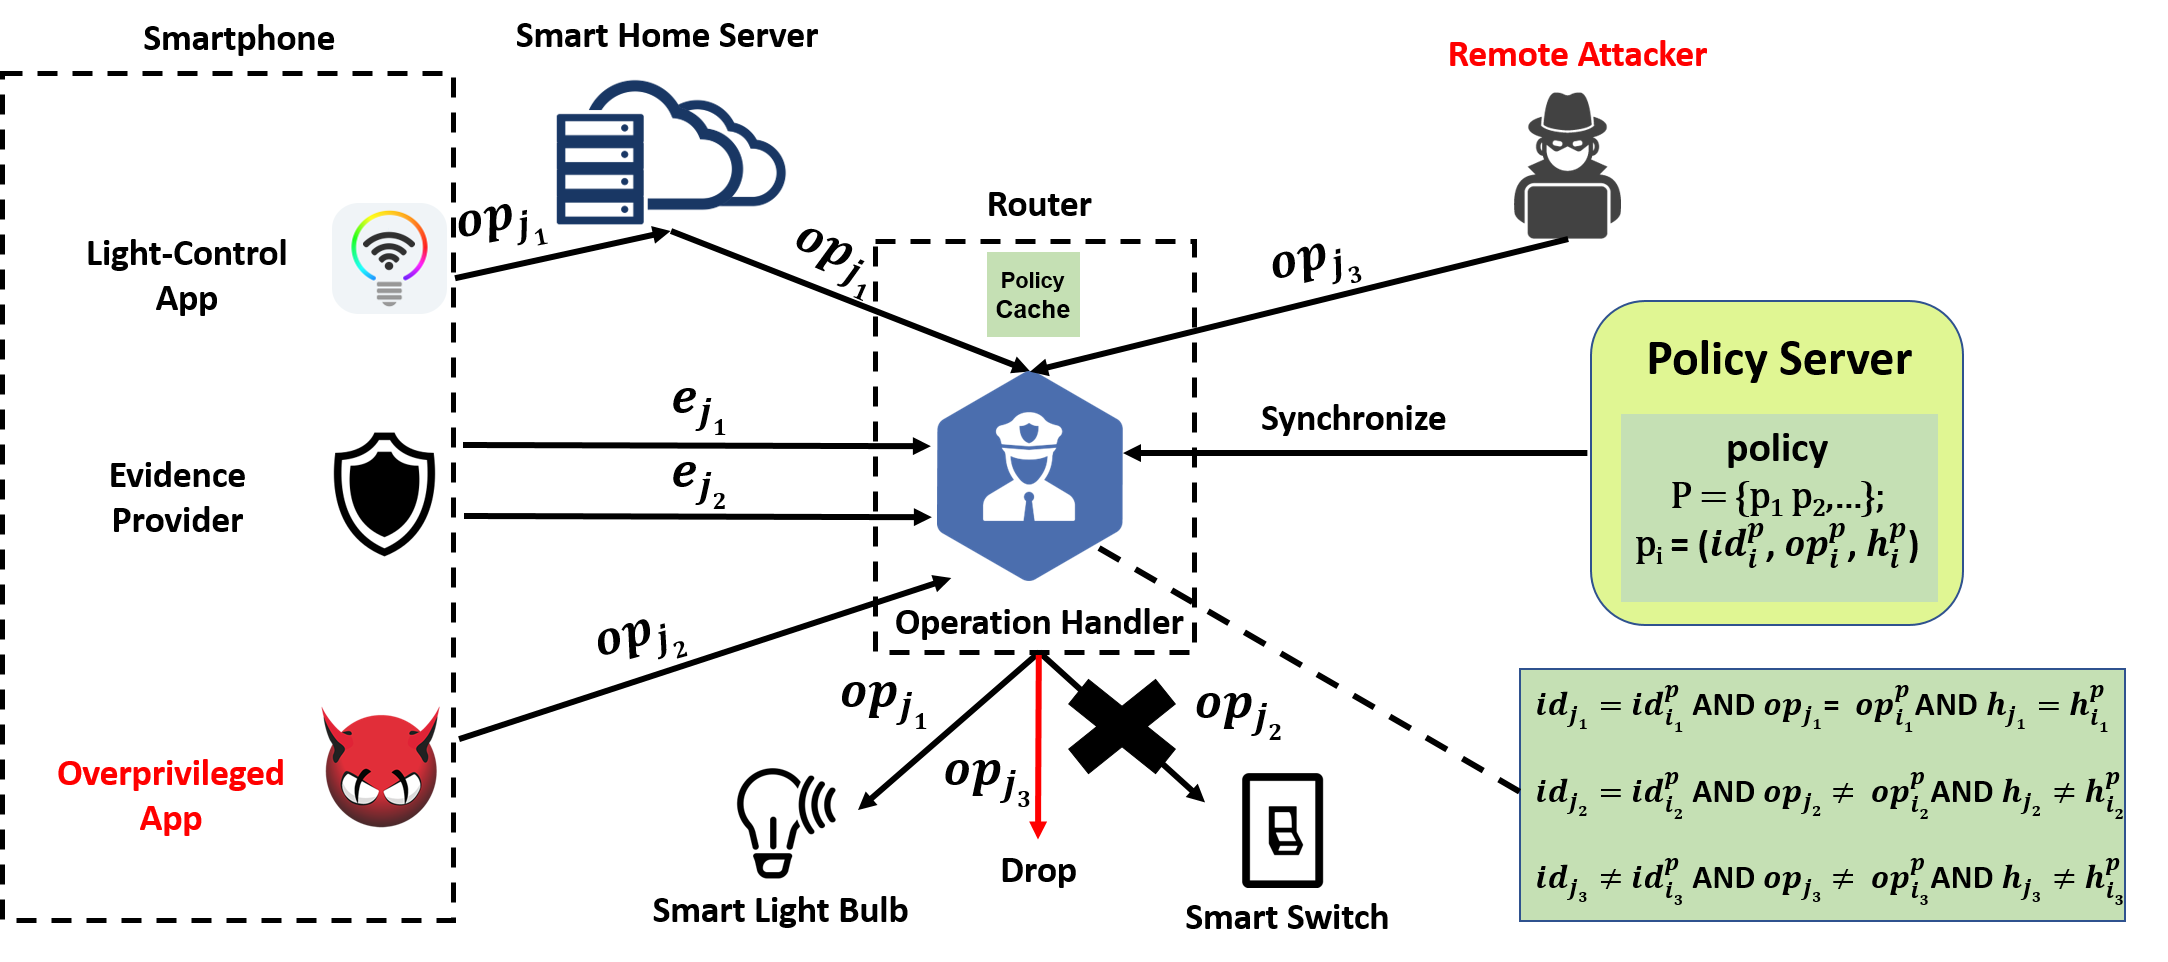
\includegraphics[scale=0.25]{examples.png}
        \caption{Three examples.}
        \label{fig:examples}
\end{figure*}

\subsubsection{Examples} \label{sec:examples}

In this subsection we employ three examples shown in Figure~\ref{fig:examples} to demonstrate how CLAF handles a legitimate operation, an operation launched by an overprivileged app, and an operation issued by an outside attacker through an open-port. 

The first example illustrates how CLAF handles a legitimate operation. In this case, the smart home app is a benign light-control app running in the user's smartphone, which is designed to control the smart light; and the evidence provider provides an evidence showing whether the user indeed uses the smart home app to turn on the light. When the user presses the ON button in the smart home app, the light-control app sends an operation $op_{j_1}$ (turning on the light) to the smart home server, which then forwards it to the operation handler. The evidence provider sends an \textit{evidence} $e_{j_1}$ corresponding to $op_{j_1}$ to the operational handler. After receiving the operation and the evidence, the operation handler first checks if the evidence is fresh; if yes, it extracts the light-control app id $id_{j_1}$, $op_{j_1}$, and $h_{j_1}$ from  $e_{j_1}$, and then compares them with the entries in the policy cache for a perfect match: if there exists a policy $p_{i_1}=(id^{p}_{i_1}, op^{p}_{i_1}, h^{p}_{i_1})$ in the policy cache such that $id_{j_1}=id^{p}_{i_1}$,  $op_{j_1}=op^{p}_{i_1}$, and $h_{j_1}=h^{p}_{i_1}$, $op_{j_1}$ is allowed to pass. By this way, the legitimate user can turn on the smart light without any problem.

The second example illustrates how CLAF handles a command from an overprivileged app. In this case, a malicious smart home app running in the user's smartphone, which was originally designed to control the user's coffee machine, attempts to open the smart switch connected to the user's garage door. Similar to the process for the legitimate operation mentioned above, the operation handler receives an operation $op_{j_2}$ (turning on the garage door switch) from the malicious smart coffee machine app and an \textit{evidence} $e_{j_2}$ associated with $op_{j_2}$ from the evidence provider. But the operation handler fails to find a perfect match in the policy cache as there is no policy allowing the coffee machine app to turn on the garage door switch. % that $p_{i_2}=(id^{r}_{i_2}, op^{r}_{i_2},h^{r}_{i_2})$ such that $id_{j_2}=c^{r}_{i_2}$ but $op_{j_2}\neq op^{r}_{i_2}$ and $h_{j_2} \neq h^{r}_{i_2}$ since the coffee app should only control the coffee machine. 
Therefore,  the operation handler denies $op_{j_2}$. By this way, an overprivileged malicious smart coffee machine app cannot turn on the garage door switch.

The third example illustrates how CLAF handles an operation launched from an open-port. In this case, a remote attacker penetrates the victim's subnet and tries to send a malicious payload $op_{j_3}$, e.g., scanning shell, to a vulnerable smart home device by exploiting an open port, say the popularly exploited port 22 by Mirai and its variants,  of the device. As the evidence provider does not send any evidence corresponding to $op_{j_3}$, the operation handler can simply drop $op_{j_3}$.



\subsubsection{Comparison with Other Defense Mechanisms.}
In this subsection, we compare CLAF with the two recently proposed IoT-specific access control mechanisms proposed to defend against the overprivilege problem: ContexIoT by Jia \emph{et al.}~\cite{jia2017contexiot} and SmartAuth by Tian \emph{et al.}~\cite{tian2017smartauth}. 

%\subsubsection{Comparison with ContexIoT}
ContexIoT is a context-based permission control scheme for appified IoT platforms. It makes a decision based on the past context of the user when an operation is detected. ContexIoT targets malicious apps or legitimate ones with overprivileged access rights, and can effectively filter out the unforeseen operations according to the previous operation decisions, by patching the app with security-specific logic to gather context info and separately consider the security sensitive behaviors. For example, as mentioned in~\cite{jia2017contexiot}, ContexIoT can successfully prevent a malicious app from opening the window when the user is sleeping, by letting the operation of turning on the window go through if the room temperature is above  $100^\circ$F while blocking if sleep mode is on. Nevertheless, ContexIoT needs time to build history, and it cannot prevent commands from compromised devices. For instance, when the room temperature is only $75^\circ$F, a compromised thermostat reports a temperature of $100^\circ$F, which triggers the smart window app to open the windows as past operations allow this app to open the windows at such a high temperature. Such an attack is completely doable; in fact, a similar attack happened recently in a casino where hackers managed to steal the casino's data by hacking into a thermostat in the fish tank~\cite{casinothero}. This attack would never happen in a smart home system protected by CLAF since compromising the thermostat requires the attacker to penetrate the smart home system with an operation containing a malicious payload, which can be prevented as illustrated by the third example presented in Section~\ref{subsec:claf-approach}. %The whole process is shown as Figure~\ref{fig:countercontexiot}.


SmartAuth matches a SmartApp's codes and its literal description based on natural language processing (NLP) to identify dishonest apps whose description does not match its real functionality. It contains a policy enforcer that needs to patch the app with discrepancies in order to regulate the activities of overprivileged and/or dishonest apps. An example given by~\cite{tian2017smartauth} indicates that SmartAuth can successfully prevent a  dishonest coffee-after-shower app from doing more (e.g., secretly opening the user's door) than making a cup of coffee for the user when the humidity in the bathroom is above a threshold (the user is taking a shower). Nevertheless, SmartAuth may fail if an attacker compromises a victim's smartphone through techniques such as \textit{ADB}, under which case the attacker can launch a legitimate smart lock app to unlock a user's door by simulating fake tapping/swiping events, as the operation is indeed from a legitimate smart lock app whose description and functionality do match, i.e., controlling door lock. Compromising a smartphone via \textit{ADB} is feasible, as we have done in our attack implementation in Section~\ref{subsec:claf-eval}. CLAF can effectively inhibit such an attack as the evidence provider in the user's smartphone cannot detect real human interaction while user-defined \textit{policies} require that real human interaction must exist for sensitive operations such as opening the door lock. %The whole process is shown as Figure~\ref{fig:countersmartauth}.

Note that both ContexIoT and SmartAuth are patching-based mechanisms targeting apps such as those on the Samsung SmartThings platform that are open source and open to modifications. However, patching-based mechanisms have little effect on a real-world smart home system in which the corresponding smart home apps (running on the smartphones) are compiled into binaries (either Mach-O for iOS or DEX for Android) and digitally signed with certificates whose private keys are known only to the authorized developers to resist code-tampering attacks. 
CLAF, on the other hand, does not make any modification to the device apps while providing at least the same protection as ContexIoT and SmartAuth do in countering the overprivilege problem; thus it has a broader application domain that covers especially the closed-source smart home systems. Moreover, CLAF can defend smart home systems from outsider attacks such as Mirai and its variants that exploit the popular open ports, which is missing by both ContexIoT and SmartAuth.

\subsection{Implementation}
\label{subsec:claf-impl}
In this subsection, we present one realization of our CLAF framework. %The basic idea is to leverage the publicly available side-channel information from a user's smartphone controller as the credential-less \textit{evidence}. %This smartphone is the controller of the smart home system that hosts all smart device apps. % via which to control the smart home system. %In the following contexts, we detail the implementations of our solution to CLAF.
%
%The reasons we leverage side-channel information 
As mentioned in Section~\ref{subsec:claf-approach}, the three components of CLAF, namely the evidence provider, the operation handler, and the policy server, are operated respectively on the users' Android smartphone, the router of the smart home system, and the secure cloud server. Upon receiving an operation, the operation handler sends an evidence request carrying the necessary information to the evidence handler, which replies with the evidence in return; then the operation handler makes the decision of passing or filtering the operation based on the user-defined policies. In the following subsections, we detail the implementation of these three components.

\subsubsection{Implementation of the Evidence Provider}
In our implementation, the evidence provider needs to collect the publicly-available side-channel information from the smart home apps as the credential-less \textit{evidence}. We choose side-channel information as evidence to realize CLAF for two reasons. First, the smart home apps running on the smartphones are unmodifiable under our consideration, and therefore we are not able to directly obtain information from the target apps by changing their codes. Second, the sandbox design of Android isolates each app in an individual process so that other apps cannot dynamically inject codes into its memory to obtain information.  Even though adopting hooking frameworks such as Xposed~\cite{xposed} and Frida~\cite{frida} to capture the activities of the target smart home apps as the \textit{evidence} may be more straightforward and more stable, such a mechanism requires either root permission or installing the target apps on a specific virtual environment, imposing a huge technical burden or even more insecurity on the user side. %Therefore, we choose to circumvent the problem by employing side-channels. Even though one can adopt injection frameworks such as Frida or XPosed, both require rooting the user’s smartphone, making the process tedious and even more insecure for the user. 
Therefore, we decide to employ a method that does not require modification of the app codes nor the root access of the smartphone. Using the publicly available side-channel information turns out to be our best option.

Note that this implementation only requests the general \texttt{INTERNET} permission from the Android system for the sake of transmitting data and requires almost zero effort from the user except launching the evidence provider app (in fact, this app can be automatically lanuched when the smart home controller app is on). %adopting side-channel based mechanisms.

\textbf{Harvesting Side-Channel Information:} 
Our goal of collecting side-channel information is to prove that an \textit{operation} towards a smart home device is indeed issued by the corresponding authorized smart home app, and that whether the \textit{operation}  is a result of human interaction. After a careful scrutiny and a few tests, we found that it suffices to harvest memory and network trace data of the target smart home app, as well as the accelerometer and the light sensor data. The reason we need the memory and network trace data of the smart home app is because we observed that when a smart home app is running, and if an operation is sent out through the Internet, the memory and the network traces change significantly, which indicates that memory and network traces are factors that are strongly correlated with the smart home app activities and thus can be used to prove whether an operation is indeed from an authorized smart home app. More specifically, we harvested the \texttt{virtual set size} (\texttt{VSS}) and \texttt{tcp\_snd}, which respectively record the virtual memory size of the target app and the amount of TCP bytes sent by the target app, and can be directly accessed through \texttt{/proc/pid/statm} and \texttt{/proc/uid\_stat/pid/tcp\_snd}, respectively, without any permission. The reason we collected the accelerometer and light sensor data is because we noticed that when a person interacts with the smartphone, these two pieces of information change significantly, which means that they are highly correlated to human interactions. Particularly, we retrieved the Z-direction data of the accelerometer and the ambient light sensor data of the smartphone by registering a callback function with \texttt{SensorEventListener}, which requires no permission.

\textbf{Generating Evidence:} 
Upon receiving an operation $op$ at time $t$, the operation handler sends an evidence request to the smartphone controller carrying $op$, the ID $app\_id$ (\texttt{uid} in Android) of the app who has launched the $op$, and $t$. Note that since we do not modify the device-specific apps hosted by the smartphone, $app\_id$ cannot be extracted from the received operation message by the operation handler; thus we simply assume that the $app\_id$ is the one for the device targeted by $op$. %, as long as the $op$ message is sent by the legitimate smartphone or the smart home server.
Upon receiving an evidence request from the operation handler, the evidence provider needs to provide the \textit{evidence} showing whether the $op$ is indeed from an authorized smart home app and whether it is the result of human interaction. For this purpose we wrote an %smartphone-based 
evidence provider app that offers the following three pieces of information for a given  time period during which $op$ occurs: (1) whether the smart home app has run; (2) whether the smart home app has launched  $op$, and (3) whether $op$ is a result of human interaction. Particularly, we consider the time period to be $n$ seconds before $t$. %, the time at which the operation $op$ was received by the operation handler. 
The pseudo-code of \textit{evidence} generation is reported in {\bf Algorithm~\ref{alg:genevid}}.

\begin{algorithm}[!htb]
\caption{\textit{Evidence} Generation.}% The overall algorithm for generating \textit{evidence}.}
\label{alg:genevid}
\begin{algorithmic}[1]
\Procedure{GenEvid}{$app\_id,op,t$}
\State $has\_run = false$
\State $has\_sent=false$
\State $has\_interact=false$
%\If {$app\_id\neq$ ``unknown''}
\State $vss\_data$ = GetVSS($app\_id$, $t-n$, $t$)
\State $tcp\_data$ = GetTcpSnd($app\_id$, $t-n$, $t$)
\State $acmt\_data$ = GetAcmt($t-n$, $t$)
\State $lght\_data$ = GetLght($t-n$, $t$)
\State $has\_run,has\_sent$ = AnalyzeAppStates($vss\_data$, $tcp\_data$)
\State $has\_interact$ = AnalyzeInteract($acmt\_data$, $lght\_data$)
%\EndIf
\State $h=(has\_run,has\_sent,has\_interact)$
\State $e=(app\_id,op, h, t)$
%\State SendEvidence($e$)
\State return $e$
\EndProcedure
\end{algorithmic}
\end{algorithm}


As shown in {\bf Algorithm~\ref{alg:genevid}}, the evidence provider takes as inputs $op$, $app\_id$, and $t$, which are extracted from the evidence request made by the operation handler. 
%Upon receiving an $op$ at time $t$, the operation handler sends an evidence request to the smartphone controller carrying $op$, $app\_id$, and $t$. Since we do not modify the device-specific apps hosted by the smartphone, $app\_id$ cannot be extracted from the received $op$ message by the operation handler; thus we simply assume that the $app\_id$ is the one for the device targeted by $op$, as long as the $op$ message is sent by the legitimate smartphone or the smart home server. % identifying $app\_id$ in the operation handler, there is no direct way of telling exactly which app launches the operation since we do not root the user's smartphone. We first check if the IP address of the operation is the one of the legitimate smartphone or the smart home server. If it is not, we denote the $app\_id$ as ``unknown''. If yes, then we assume the  $app\_id$ to the the app  associated with the smart home device which the operation targets. 
%For example, if the operation is opening the light, and the IP address of this operation is the smartphone, then we let the $app\_id$ to be the ID of light-control app. 
%After receiving an evidence request,
The evidence provider first initializes the evidence boolean variables  (lines 2-4), then retrieves the target app's \texttt{VSS} data and \texttt{tcp\_snd}, as well as the system's accelerometer and light sensor data for the time duration from $t-n$ to $t$ (lines 5-8). Next the evidence provider feeds these four pieces of side-channel data to the functions \texttt{AnalyzeAppStates()} and \texttt{AnalyzeInteract()}, which return the boolean values indicating whether the target app has run, whether it has sent an \textit{operation}, and whether human interaction has happened (lines 9-10). Afterwards, the evidence provider constructs and returns the \textit{evidence} associated with this operation $op$ based on Definition 1, where $h$ consists of the three boolean values generated by the two functions \texttt{AnalyzeAppStates()} and \texttt{AnalyzeInteract()} (lines 11-13). %Finally, the evidence provider pushes the \textit{evidence} to the operation handler (line 14).

\textbf{Analysis on the App States:} 
In a typical smart home system, if a user wants to launch an operation through the smart home app, the smart home app would send out a series of TCP packets containing the operation to the target smart home device or to the smart home server. In this process, two requirements need to be satisfied in order to tell if an operation does come from the smart home app: (1) the smart home app has actually run, and (2) the smart home app has actually sent out TCP packets. Correspondingly, \texttt{VSS} and \texttt{tcp\_snd} change in the designated period of time. Note that a third party app such as our evidence provider is not allowed to monitor the real TCP traffic of another app due to the sandbox design of the modern operating systems unless it acquires the root permission or installs a proxy server on the user's smartphone. Nevertheless, these two methods not only are tedious but also pose additional security threats for a user; thus we choose to analyze the publicly available \texttt{tcp\_snd}, which is secure and lightweight.
Based on the above discussion, we present our algorithm for analyzing the app states in {\bf Algorithm~\ref{alg:alzapp}}.

\begin{algorithm}[!htb]
\caption{Analyzing App States: Analyze if the target app has run or if it has sent out TCP traffics.}\label{alg:alzapp}
\begin{algorithmic}[1]
\Procedure{AnalyzeAppStates}{$vss\_data$, $tcp\_data$}
\State $has\_run = false$
\State $has\_sent = false$
\If {$vss\_data \neq \emptyset$ AND $tcp\_data \neq \emptyset$}
\State $min\_vss = \min(vss\_data)$
\State $max\_vss = \max(vss\_data)$
\State $min\_tcp = \min(tcp\_data)$
\State $max\_tcp = \max(tcp\_data)$
\If{$max\_vss-min\_vss \geq \delta_{1}$}
\State $has\_run = true$
\EndIf
\If{$max\_tcp-min\_tcp \geq \delta_{2}$}
\State $has\_sent = true$
\EndIf
\EndIf
\Return $has\_run$, $has\_sent$
\EndProcedure
\end{algorithmic}
\end{algorithm}

As shown in {\bf Algorithm~\ref{alg:alzapp}}, the evidence provider first initializes two boolean variables and checks if the input $vss\_data$ is empty since in Android $vss\_data$ is empty if the target app is not launched (lines 2-4). Note that $tcp\_data$ in $\backslash$\texttt{proc} cannot be empty whether or not an app is running as it accumulates all the TCP traffic data. If there exists non-zero $vss\_data$, the evidence provider first calculates the minimum and maximum values of $vss\_data$ and $tcp\_data$ and then takes the differences between them (lines 5-8). If the difference between the maximum value and the minimum value of $vss\_data$ is greater than or equal to a predetermined threshold $\delta_1$, this guarantees that the smart home app is actively running on the foreground other than passively sitting in the background (lines 9-10). Similarly, if the difference between the maximum value and the minimum value of $tcp\_data$ is greater than or equal to a predetermined threshold $\delta_2$, it proves that the smart home app indeed sends a series of TCP packets (lines 11-12).

\textbf{Inference of Human Interactions:} 
Our algorithm for inferring the human interaction is based on changes in the accelerometer and light sensor data. When a user is using a smartphone, all interactions can be categorized into two types: tapping and swiping. Based on our observation, whenever tapping or swiping happens, the accelerometer data at the Z-direction, i.e., the direction at which the gravitational acceleration points,  changes drastically. This is because when a person taps or swipes on the screen, he imposes a force on the smartphone at the gravitational direction. According to the Newton's Second Law, the acceleration on the Z-direction would increase under this situation. We also observed that the light sensor data has a slightly abrupt change whenever tapping or swiping occurs. This is because a sudden movement of the smartphone incurs a difference in light absorption of the light sensor. However, even though we noticed that changes in this side-channel data can reflect whether or not human interactions exist, pure numerical analysis cannot handle the job effectively because sensor data always contain heavy noises. Therefore, we adopted five typical machine learning models, namely support vector machine (SVM), decision tree (DT), multilayer perceptron (MLP), random forest (RF), and  Adaptive Boosting (AdaBoost), for inferring whether a human interaction has occurred based on the given sensor data. Each of the models outputs a binary prediction, 0 or 1, representing a human interaction has not or has occurred, respectively. We further took the majority vote ensemble of the five machine learning models to reduce the effect of biases and overfitting. Note that the adopted machine learning models have high computational overhead at the training phase; therefore, we trained the models offline and employed them to make real-time predictions. The pseudocodes for the human interaction inference are presented in {\bf Algorithm~\ref{alg:infint}}.

%Based on the discussions mentioned above, we present our algorithm for inferring whether or not human interactions exist in {\bf Algorithm~\ref{alg:infint}}.

\begin{algorithm}[!htb]
\caption{Inferring Human Interactions: infer if a human interaction has occured.}\label{alg:infint}
\begin{algorithmic}[1]
\Procedure{AnalyzeInteract}{$acmt\_data$, $lght\_data$}
\State $m_l=lght\_data.len$
\For{$i=1\ to\ m_l-1$}
\State $lght\_data[i]=lght\_data[i+1]-lght\_data[i]$
\EndFor
\State $lght\_data[m_l]=\emptyset$
\State $z\_data=acmt\_data.z$
\State $z\_data=FFT(z\_data)$
\State $x = concat(z\_data,lght\_data)$
\State $svm\_y$ = svm\_predict($x$)
\State $dt\_y$ = dt\_predict($x$)
\State $mlp\_y$ = mlp\_predict($x$)
\State $rf\_y$ = dt\_predict($x$)
\State $ada\_y$ = adaboost\_predict($x$)
\State $y=svm\_y+dt\_y+mlp\_y+rf\_y+ada\_y$
\If{$y\geq3$}

\Return true
\Else

\Return false
\EndIf
\EndProcedure
\end{algorithmic}
\end{algorithm}

As shown in {\bf Algorithm~\ref{alg:infint}}, the evidence provider first alters the light sensor data by subtracting from each value its successor value (lines 2-4). The reason for doing this is to eliminate the influence of the brightness level of the ambient environment because the lighting level is highly sensitive to the ambient environment and thus directly using the original light data for analysis could result in an incorrect prediction. Therefore, we employ the difference data that is less affected by the environment. Next the evidence provider retrieves the Z-direction accelerometer data and processes it with the Fast Fourier Transform (FFT) shown as follows:
\begin{equation}
Z_k = \sum_{j=0}^{m_{z}-1}z_{j}e^{-i2\pi kj/m_{z}},\ \ k=0,\cdots,m_{z}-1,
\end{equation}
where $m_{z}$ is the number of total elements in the Z-direction accelerometer data, $z_j$ is the $j-th$ element of the original Z-direction accelerometer data, and $Z_k$ is the $k-th$ element of the Fourier transformed data (lines 5-7). Finally, the evidence provider concatenates the Fourier transformed Z data and the modified light data as a vector of new data, feeds it to the five machine learning models, and makes a final decision based on the majority vote (lines 8-16). 


\subsubsection{Implementation of the Operation Handler}
Based on our previous description of the operation handler, one can see that its main task is to allow or deny an operation. Therefore, the core function of the operation handler is to process the passing traffics. Our implementation of the operation handler runs on the gateway of the user's home router.

%\subsubsection{Relaying Traffics}
Processing a traffic at the operation handler is actually a combination of intercepting the traffic %filtering the traffic, re-creating it, 
and then filtering or forwarding it to the designated party. %Re-creating a traffic is trivial to realize as one only needs to reproduce a copy of the filtered traffic. However, 
Filtering a traffic is non-trivial even though the operation handler runs on the router since the router does not have a direct way for dropping network packets. We managed to circumvent this problem by first activating the \texttt{iptable} and adding a rule at the \texttt{PREROUTING}, a chain where packets enter before a routing decision is made, to redirect any traffic that goes into the smart home devices to a designated port on the router~\cite{purdy2004linux}. However, the \texttt{iptable} alone is not sufficient to filter the traffics since Linux kernel only allows \texttt{iptable} to manipulate the packets whose source or destination IP address is that of the router itself. One may resolve this issue by revising the kernel codes and re-compile them on the user's router kernel. Nevertheless, it is not realistic in practice to re-program the users' routers. We managed to overcome this problem by exploiting ARP spoofing, a technique that targets the data link layer and can bind an IP address with our designated MAC address, to successfully convince the router that our operation handler has the IP address which in fact belongs to the target smart home device. In other words, by combining \texttt{iptable} and ARP spoofing, we managed to realize the ability of filtering arbitrary traffics. 

There still exists a subtle issue we need to handle, i.e., how to process the encrypted traffics. Even though many smart home systems do not encrypt network traffics within the LAN based on our observation, some do use SSL/TLS encryption. Thus we further implemented a rule based on which the \texttt{iptable} can direct all the encrypted traffics to a designated port where we conduct a man-in-the-middle (MITM) key exchange hijack to force the encryption/decryption to use our certificate.  MITM key exchange hijack, though is regarded as an attack, is completely doable, and in fact is widely used in many areas besides creating threats. For example, it is reported that Iranian government uses this technique to monitor its citizens for the contents they searched in Google, which are well protected with HTTPS~\cite{iranmitm}. There are also many off-the-shelf products such as mitmproxy and SSLsplit that employ this technique and have been extensively adopted in industry~\cite{mitmproducts}. While in our implementation, we used a similar logic by creating a python program with no more than 200 lines of codes combined with \texttt{iptable}. It is shown in Section~\ref{subsec:claf-eval} that all HTTPS traffics of the 137 SmartApps can be successfully intercepted and decrypted by our implementation without any obstacle. Finally, the operation handler decides whether to drop or to pass a traffic based on the \textit{policies} synchronized with the policy server.

\subsubsection{Implementation of the Policy Server}
The policy server is capable of synchronizing \textit{policies} with those in the policy cache of the operation handler and accepting \textit{policy} updates. To synchronize the \textit{policies}, the policy server needs to push a list of \textit{policies} to the operation handler whenever its maintained \textit{policies} are updated. As mentioned in Section~\ref{subsec:claf-approach}, \textit{policies} need to be updated (1) when a new device enters the system; (2) when a firmware is updated; and (3) when a user decides to modify the \textit{policies} based on his will. Since our \textit{policies} are user-defined, the user needs to manually update the \textit{policies} whenever one of the three situations mentioned above happens. 

We implemented our policy server on the Samsung SmartThings platform with the RESTful API as a web service SmartApp~\cite{smartthings}. We chose SmartThings as the platform to implement the policy server for two major reasons: i) it is the largest programming platform for smart home systems and supports most of the smart home products available on the market; ii) it is a cloud-based platform using HTTPS and access tokens for security maintenance thus a user can safely manage the \textit{policies} list by adding or deleting entries. Note that the policy server can also be implemented on other smart home platforms such as Google Actions~\cite{googleaction} and Amazon Skills~\cite{amazonskill}. But since these platforms are not as popular as SmartThings, and they are not convenient as Google Actions requires users to possess Google Assistant while Amazon Skills needs Alexa Speaker to interact with the platforms, we chose to implement our policy server on the SmartThings platform.

\subsection{Evaluation}
\label{subsec:claf-eval}
In this section, we report the evaluation results of our realization of CLAF. We first describe the experimental environments and the corresponding attack settings under our consideration. Then we evaluate the accuracies of {\bf Algorithm~\ref{alg:alzapp}} and {\bf Algorithm~\ref{alg:infint}}, and the effectiveness of our approach in countering various attacks. Finally we present the performance overhead of our approach in terms of running times. Note that we do not compare our approach with SmartAuth and ContexIoT since they are both offline patching-based mechanisms while our CLAF realization does not need to make any modification to the smart home device firmwares.

\subsubsection{Experimental Setup}
%In this subsection, we describe the environments of the three experiments: a typical real-world smart home system that employs a smartphone as a controller hosting all the smart device apps, an environment that supports the SmartApps on the Samsung SmartThings platform, and an environment that  Mirai and its variants.
In this subsection, we first describe a real-world smart home system to test the effectiveness of our CLAF realization in countering the four attacks presented in Subsection~\ref{sec:preliminaries} as well as Mirai and its variants. Since ContexIoT and SmartAuth both target the SmartApps on the Samsung SmartThings platform in defending against the overprivilege problem, we  conducted experiments to demonstrate how our CLAF realization can protect SmartApps from both the open-port and the overprivilege attacks. 

%\subsubsection{Settings of the Experiments based on Real-World Smart Home Systems}
\textbf{A Real-World Smart Home System.} 
We set up a typical real-world smart home system containing the following seven popular smart home devices: a Google Home Speaker, a WeMo Mini Smart Plug, a Belkin Insight Smart Plug with Energy Monitoring, a Tuya Smart Switch, a TP-LINK Smart Light Bulb, a TP-LINK Smart Switch, and an Apple Home Pod. Besides these seven full-fledged devices, we also included two Raspberry Pis, denoted by A and B, for simulating more general IoT devices. Note that it is a common practice to use a Raspberry Pi to simulate a smart home device since most IoT devices use ARM processors and a Raspberry Pi is a tiny programmable module that adopts the ARM instruction set. In our setting, Raspberry Pi A is employed as a regular smart home device while Raspberry Pi B is used as a compromised one. %device to be explained in the later context. 
We further employed two Android devices for our evaluations: an Amazon BLU R2 smartphone and a Google Nexus 7. The configuration of this experimental smart home system is illustrated in Figure~\ref{fig:smarthomesys}. 

We summarized the specifications of the smart device operations under our consideration in Table~\ref{tbl:oplist}. Note that even though a smart home device can have many operations, we chose the most important and sensitive one for each of the seven smart home devices.

We also tested our approach against the most rampant IoT-specific botnet virus, the Mirai and its variants, with this real-world smart home system. Since both Mirai and its variants target specific open ports and vulnerabilities that our selected real-world smart home devices do not have, we used Raspberry Pi A to open the designated vulnerable ports and simulated the functions targeted by Mirai and its variants.

\begin{table*}[!htb]
\centering
\caption{Summarized List of Operation Specifications}
\label{tbl:oplist}
\resizebox{\columnwidth}{!}{%
\begin{tabular}{|c|c|c|c|c|c|c|c|}
\hline
                                                                & \begin{tabular}[c]{@{}c@{}}Google Home\\ Speaker\end{tabular}                              & \begin{tabular}[c]{@{}c@{}}WeMo Mini\\ Smart Plug\end{tabular} & \begin{tabular}[c]{@{}c@{}}Belkin Insight\\ Smart Plug\end{tabular}                   & \begin{tabular}[c]{@{}c@{}}Tuya Smart\\ Switch\end{tabular} & \begin{tabular}[c]{@{}c@{}}TP-LINK Smart\\ Light Bulb\end{tabular} & \begin{tabular}[c]{@{}c@{}}TP-LINK\\ Smart Switch\end{tabular} & \begin{tabular}[c]{@{}c@{}}Apple Home\\ Pod\end{tabular} \\ \hline \hline
\begin{tabular}[c]{@{}c@{}}Operation Specific\\ Term\end{tabular} & \texttt{scan\_wifi}                                                                      & \texttt{SetBinaryState}                                      & \texttt{GetInsightParams}                                                           &      \texttt{switch}                                                       & \texttt{transition\_light\_state}                                & \texttt{set\_relay\_state}                                   &      \texttt{pair-setup}                                                                                      \\ \hline
\begin{tabular}[c]{@{}c@{}}Operation\\ Description\end{tabular} & \begin{tabular}[c]{@{}c@{}}Scan and return \\ a list of\\ amibient Wi-Fi AP\end{tabular} & Turn on or off                                                 & \begin{tabular}[c]{@{}c@{}}Get a user's\\ electricity\\ consumption data\end{tabular} &                                                            Turn on or off & Turn on or off                                                     & Turn on or off                                                 &                                         \begin{tabular}[c]{@{}c@{}}Pair up with\\ device for airplay\end{tabular}
 \\ \hline
Open Port                                                       & 8008                                                                                       & 49153                                                          & 49153                                                                                 &  6668                                                           & 9999                                                               & 9999                                                           &                                                         7000 \\ \hline
SSL/TLS Encrypted                                               & No                                                                                         & No                                                             & No                                                                                    & No                                                            & No                                                                 & No                                                             &                                                         No \\ \hline
\end{tabular}
}
\end{table*}


\begin{figure}[!htb]
        \centering
        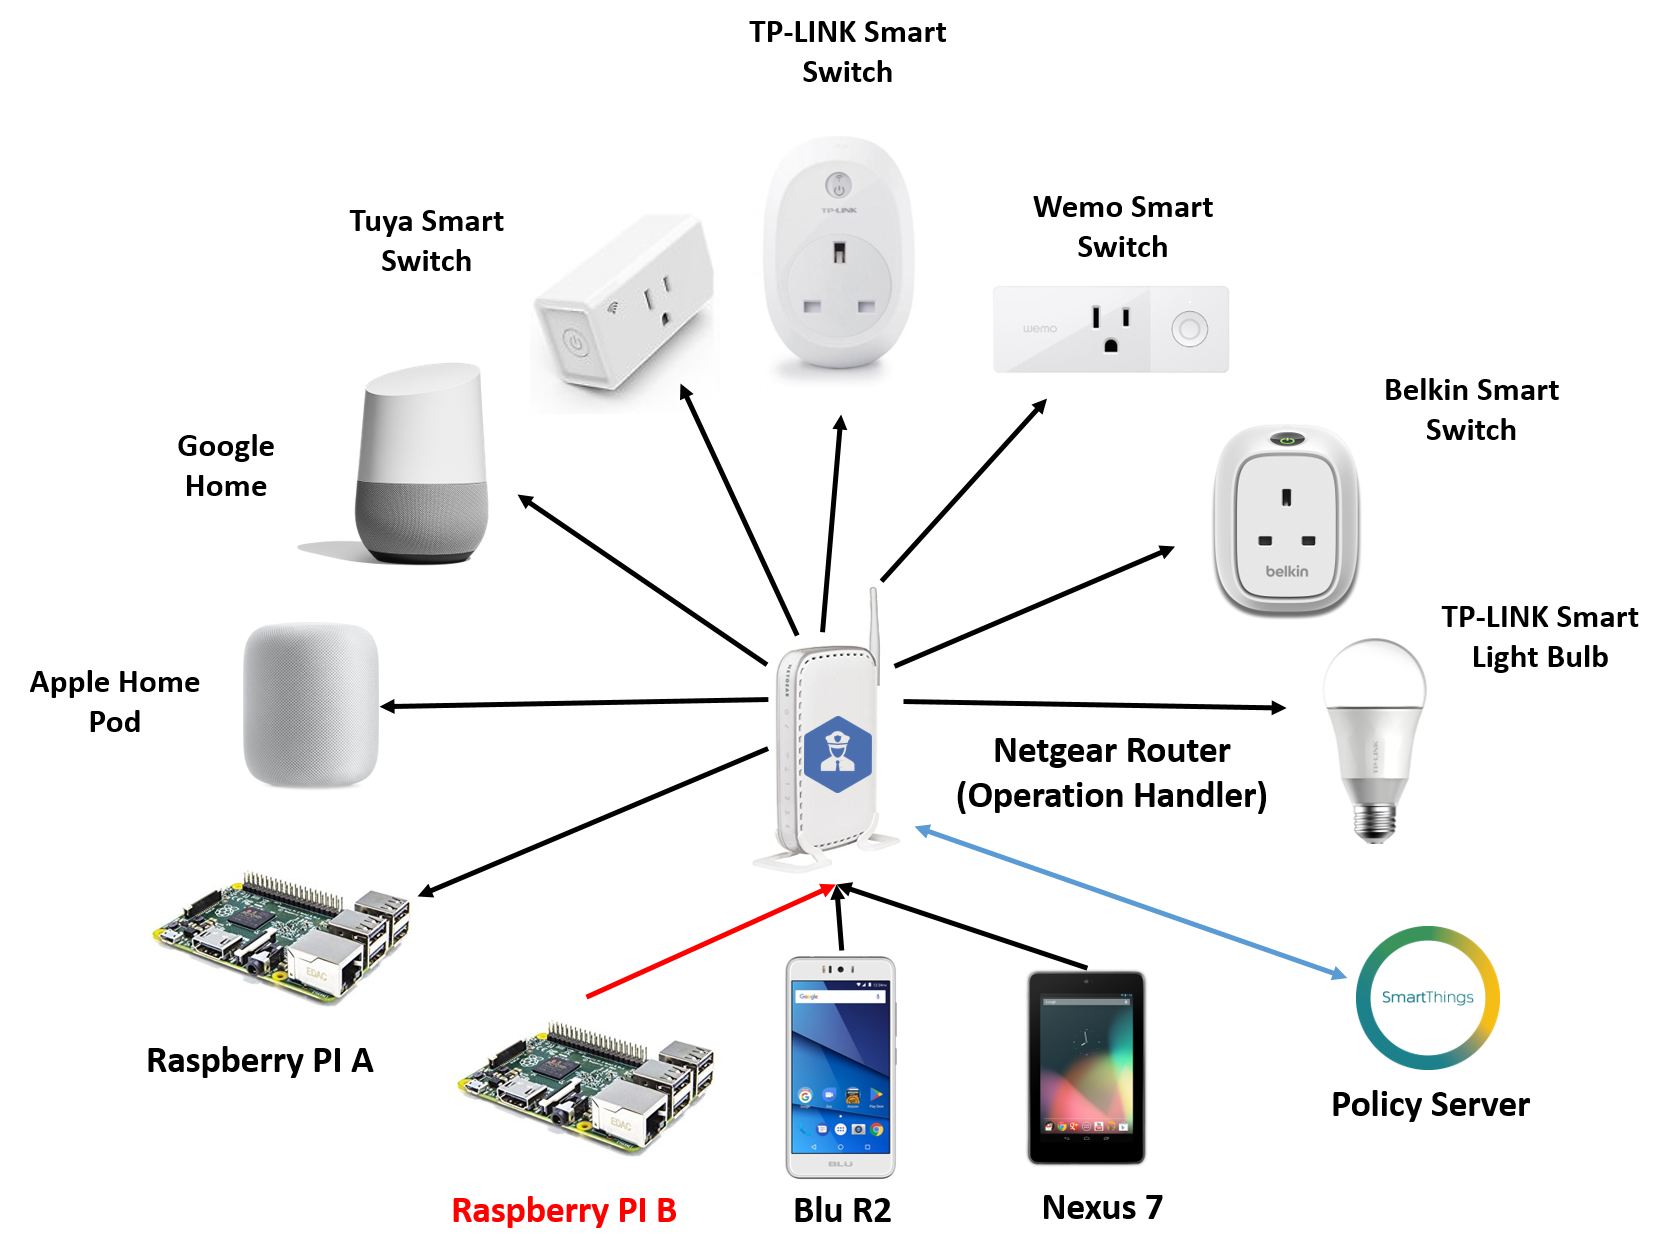
\includegraphics[width=0.5\textwidth]{smarthomesys.png}
        \caption{The configuration of our experimental smart home system.}
        \floatfoot{The two smartphones are the controllers on which the smart home apps running, and Raspberry Pi B serves as a compromised device (attacking source) in our experiment.}
        \label{fig:smarthomesys}
\end{figure}

\textbf{Experiments on SmartApps.} 
Besides setting up the real-world smart home system, we also manually collected 553 SmartApps from the official development community of the Samsung SmartThings platform~\cite{smartthingscommunity}, and conducted evaluations on our CLAF realization to defend SmartApps against attacks exploiting the open-port and overprivilege problems.

\begin{itemize}

\item \textbf{Defending Against the Open-Port Attacks.} 
To evaluate the defense of our CLAF realization against the attacks  exploiting the open-port problem, we selected 137 of the 553 SmartApps which involve data communications, i.e., containing \texttt{mappings} or \texttt{path} in their Groovy codes. Then we wrote an automatic program to parse the operations in these apps and fed the apps to the Samsung SmartThings IDE simulator for testing purpose. Note that in this environment, the traffics are all encrypted with HTTPS; therefore, we leveraged the MITM traffic hijacking technique as we mentioned in Section~\ref{subsec:claf-impl} to decrypt the ciphertexts. We found that all the HTTPS traffics of the 137 apps can be decrypted without any obstacle.

\item \textbf{Defending Against the Overprivilege Attacks.} 
To evaluate the defense of our CLAF realization against the attacks exploiting the overprivilege problem, we manually identified 58 potentially overprivileged SmartApps from the 553 collected ones. The principle we used to figure out an overprivileged SmartApp is to match its description with the real permissions it requests in its codes. The \texttt{description} tag is located  in the block of \texttt{definition} and the real permission request is located in the \texttt{preferences} block under the \texttt{section} tag with the format shown as follows:
\begin{lstlisting}
section("section notes") {
    input "sensor_alias", 
    "capability.sensortype" }
\end{lstlisting}
where the term \texttt{capability.sensortype} indicates the type of the sensor the SmartApp uses. Obviously, by matching the \texttt{capability.sensortype} and the \texttt{description} one can manually uncover potential overprivileged SmartApps. One example of an uncovered overprivileged SmartApp has a description saying that the SmartApp changes the Smart Hues to different colors based on different weather forecasts; but the SmartApp accesses a user's motion sensor by declaring \texttt{capability.motionSensor}. In this case, we consider the SmartApp overprivileged. Besides these 58 overprivileged SmartApps we uncovered, we also used 10 overprivileged SmartApps created by Jia \emph{et al.}~\cite{jia2017contexiot}. Therefore, we have in total 68 overprivileged SmartApps for our experiments.
%\subsubsection{Setting of the Experiments based on Mirai and Its Variants}
%We also testified our approach against the most rampant IoT-Specific botnet virus, the Mirai, and its variants. Since both Mirai and its variants target specific open ports and vulnerabilities that our selected real-world smart home devices do not have, we used Raspberry Pi A to open the designated vulnerable ports and simulated the functions targeted by Mirai and its variants target.
\end{itemize}

\subsubsection{Settings of the Attacks}
%Based on our threat models, an attacker can implement various attacks.  
In this subsection, we first detail our implemented attacks for the experimental environments based on the four threat models presented in Section~\ref{sec:preliminaries}; then we present the attacks on SmartApps of the Samsung SmartThings platform.

\textbf{Attacks on the Real-World Smart Home System.} 
Our attacks against the real-world smart home devices can be categorized into two types, attacks on full-fledged smart home devices and attacks based on Mirai and its variants.

\begin{itemize}

\item \textbf{Attacks on Full-Fledged Smart Home Devices.}
We constructed and fully implemented four attacks based on the four threat models for our real-world smart home devices, with one attack for each threat model. We let each attack launch the seven operations detailed in table~\ref{tbl:oplist} to the corresponding target devices in our smart home system. To construct an attack based on the first threat model, the attacker must penetrate the victim's subnet from the external network. In order to realize this, we drafted a malicious program in which we created a reverse shell directed to our attacking machine (a PC running on Ubuntu 16.04) based on the \texttt{ARM} instructions. Then we ran the malicious program on the Raspberry Pi B in our smart home system. Next we commanded the Raspberry Pi B to create and send arbitrary operations. For the second threat model, we first penetrated the subnet as we did for the first threat model; then we tampered the IP of the Raspberry Pi B and made it the IP of the victim's smartphone by altering the IP segment, located in the network layer header, of the Raspberry Pi B. We leveraged \texttt{hping3} 
%, a network penetration tool, 
to accomplish this IP spoofing attack~\cite{hping3}. For the third threat model, we created a malicious Android app that \emph{only} requires the \texttt{INTERNET} permission to send out operations. This malicious app, which could be an overprivileged one, also launches benign target smart home apps as camouflages while sending malicious operations using the \texttt{startActivity} API call. Our implementation of the last threat model exploits the Android \texttt{ADB} through USB. We assume that the victim's smartphone is plugged into our compromised device (Raspberry Pi B) in this case for power charging, and the attacker would secretly launch the target smart home apps through \texttt{adb} \texttt{shell} and trigger the operations on the apps by simulating the designated inputs e.g., tapping and swiping through the \texttt{input tap} and \texttt{input swipe} commands, respectively.

\item \textbf{Attacks based on Mirai and Its Variants.}
Mirai and its variants are powerful malwares that are, in fact, affiliated with the description of the first and second threat models. Mirai has many variants; we chose the two most infamous ones, namely Satori~\cite{miraiwiki} and IoT\_reaper~\cite{iotreaper}, for constructing our attacks. Since Mirai and its variants do not have the functions to compromise a smartphone, and also because many of the malicious payloads such as the buffer overflow ones would never appear in a smartphone environment, there is no need to create attacks based on the third and the fourth threat models. For Mirai, we managed to download its source codes on the Github. Note that Mirai includes many tedious codes that are not relevant with attacking any IoT device such as arbitrarily launching DDoS to some infrastructures' servers; thus we amended the codes to restrict Mirai only to attack our designated smart home device (Raspberry Pi A). On the other hand, since the source codes of Satori and IoT\_reaper are not available online, we recreated simulated attacks based on their binaries. Satori exploits two CVE vulnerabilities and IoT\_reaper exploits eight CVE vulnerabilities known so far. Finally, we collected all the malicious payloads these three viruses use and simulated two attacks for each virus based on the first and the second threat models. Note that for these attacks, Raspberry Pi B serves as the attacking source while Raspberry Pi A works as the attacking target.

\end{itemize}

\textbf{Attacks on SmartApps of the Samsung SmartThings Platform.} 
We consider two types of attacks on the SmartApps of the Samsung Smartthings platform, namely open-port attacks and overprivilege attacks.
\begin{itemize}

\item \textbf{Open-Port Attacks.}  We created two attacks based on the first and second threat models to evaluate our approach for defending the 137 SmartApps against the open-port attacks. The corresponding attack implementations are very similar to those mentioned above for the real-world smart home system. Note that since there is no actual smartphone apps corresponding to the SmartApps run in the Samsung SmartThings server, it is not feasible to create attacks based on the third and fourth threat models; thus we let function \texttt{AnalyzeAppStates} always return true for our evaluation purpose. The operations in each SmartApp are defined in the \texttt{mapping} section of the codes with the format of \texttt{path(/operation)}. Our attacks automatically extract the designated operation according to the format and dynamically construct payloads.

\item \textbf{Overprivilege Attacks.} Since we do not have the physical smart sensors targeted by the SmartApps, we used Raspberry Pi A to emulate 22 different types of sensors including motion sensor, contact sensor, switch, presence sensor, humidity sensor, and so on, for testing purpose. Then we adopted the 68 overprivileged SmartApps locally in a simple simulator we wrote with Python which parses the requested sensors and their corresponding operations, and sents the operations, e.g., turning on switch, to the Raspberry Pi A. These overprivilege attacks are based on the third threat model since the overprivileged SmartApps are considered as malicious ones. Because our evaluation was running on an emulated environment, we considered the return values of \texttt{AnalyzeAppStates} and \texttt{AnaylyzeInteract} to be true.

\end{itemize}

\subsubsection{Accuracies of the Main Algorithms}
To evaluate our algorithm {\bf Algorithm~\ref{alg:genevid}}, we set $n=3$, which indicates that we retrieve the side-channel data 3 seconds before the time when an operation is received by the operation handler as mentioned in Section~\ref{subsec:claf-impl}. Note that we tried other values of $n$ and found that $n=3$ yields satisfiable results. Also note that even though both \texttt{VSS} and \texttt{tcp\_snd} have high values most of the time based on our observations, we considered the possibility that a user may clear the cache data of his smartphone from time to time; thus we set both $\delta_1$ and $\delta_2$ in {\bf Algorithm~\ref{alg:alzapp}} to a relatively small value, 100 in our case, to ensure robustness.

\textbf{Accuracy of Analyzing the App States.} 
To analyze the accuracy of the function \texttt{AnalyzeAppStates} of {\bf Algorithm~\ref{alg:alzapp}}, we wrote an automated program based on \texttt{ADB} that launches the seven target smart home apps as well as the corresponding operations shown in Table~\ref{tbl:oplist}, and an additional testing smart home app for Raspberry Pi. For each smart home app, we collected 4,000 pieces of \texttt{VSS} and \texttt{tcp\_snd} data lasted for 3 seconds for both Android smartphone devices (2,000 pieces of data for each device). In each of these 4,000 data pieces, 2,000 were collected at the times when the target app was not actively running and the other 2,000 were at the times when the target app was actively running and sent a target \textit{operation}. Therefore, we collected in total 32,000 pieces of \texttt{VSS} and \texttt{tcp\_snd} data (for eight devices). Then we fed these 32,000 pieces of data into  {\bf Algorithm~\ref{alg:alzapp}} and compared the output results with the ground truth. We achieved an overall accuracy of 99.58\% (31,866 out of 32,000 are accurately analyzed), with no false positives and a 0.84\% false negative rate (134 out of 16,000). The detailed results for each smart home app are illustrated in Figure~\ref{fig:appstate}. As one can see, our algorithm for analyzing the app states is highly accurate.

\begin{figure*}[!htb]
        \centering
        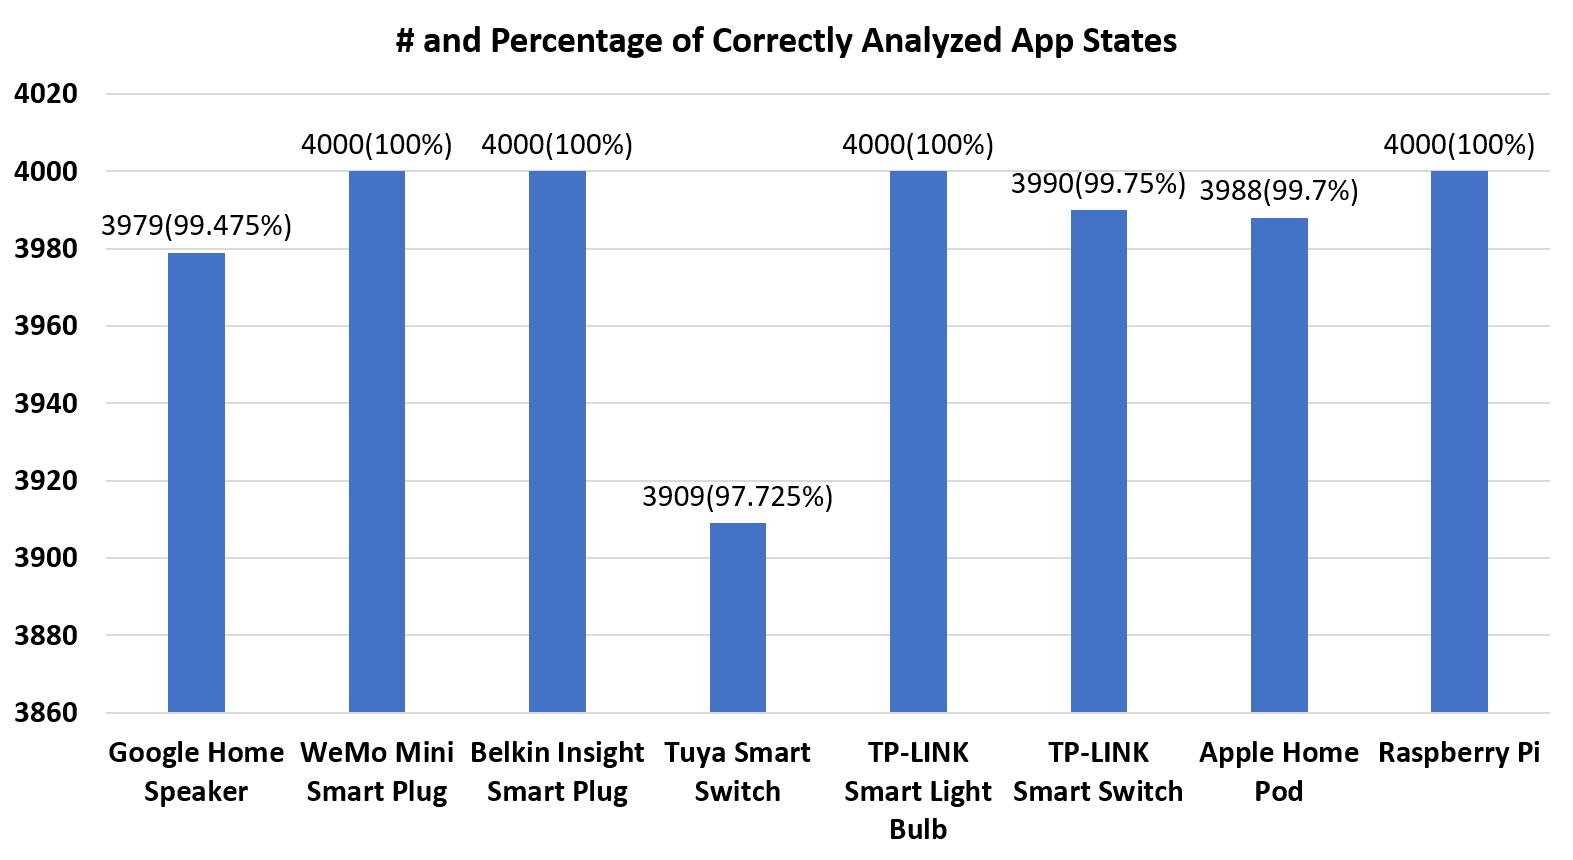
\includegraphics[width=0.9\textwidth]{appstate.png}
        \caption{The numbers and percentages of correctly analyzed app states by our algorithm.}
        \label{fig:appstate}
\end{figure*}

\textbf{Accuracy of Inferring Human Interactions.} 
Since our algorithm for inferring human interactions detailed in Section~\ref{subsec:claf-impl}, i.e., {\bf Algorithm~\ref{alg:infint}}, relies heavily on machine learning, we need to collect ground truth data for training and testing in order to build the learning models. In order to do so, we wrote a training app that randomly generates an event asking a volunteer to tap or swipe somewhere on the smartphone screen and constantly collecting the accelerometer and light sensor data, with each collection lasting for 3 seconds. We then recruited 13 volunteers to interact with our written training app on the two Android devices for data collection. The volunteers were asked to perform tapping or swiping randomly on the screen approximately once every 6 seconds so that we can have roughly half of the data containing human interactions. Finally, we collected 12,630 pieces of accelerometer and light sensor data, among which 6,541 (51.79\%) of them were collected while the volunteers were interacting with our app and the other 6,089 (48.21\%) were collected while the volunteers were not interacting with our app. 

Next, we conducted cross-validation by randomly separating the 12,630 data into ten folds, with each containing 1,263 pieces of data; then we used nine folds for training and the left-over fold for testing. We repeated the cross-validation process for 100 times and the averaged accuracy of these testings is 91.21\%.

Besides the evaluation based on cross-validation, we asked 3 volunteers to actually interact with the real smart home apps and launched the corresponding operations as listed in Table~\ref{tbl:oplist}. We collected the accelerometer and light sensor data at the same time, with each piece of data corresponding to 3 seconds. We obtained 4,128 pieces of data in total, among which 2,012 (48.74\%) were collected while the volunteers were actually interacting with the apps and triggering the target operations, and the other 2,116 pieces of data (51.26\%) were collected otherwise. Then we trained our ensembled machine learning model with all the 12,630 pieces of data obtained above and fed the 4,128 pieces of data for testing. Our model achieves an accuracy of 89.34\% (3,688 out of 4,128), with 4.77\% false positive rate (101 out of 2,116) and 16.8\% false negative rate (339 out of 2,012).

\subsubsection{Effectiveness in Defending Against Attacks}
In this subsection, we evaluate the effectiveness of our approach to protect our experimental real-world smart home system as well as the SmartApps of the Samsung SmartThings platform against the attacks presented in Section~.

\textbf{Experiments on the Real-World Smart Home System.} 
We launched each of the four attacks for each of the devices in the smart home system for 100 times. We also interacted with each smart home app and sent the corresponding operations for 100 times. Therefore, we conducted in total 3,500 trials among which 2,800 ($4\times 7\times 100$) are attack ones and 700 are legitimate ones. The results indicate that our approach successfully defended against 98.68\% of the attack trials (2,763 out of 2,800) and recognized 90.14\% of the legitimate ones (631 out of 700). Since roughly 10\% of the legitimate operations were classified as unauthorized ones, we added an additional step by implementing a UI activity in the user's smartphone, which allows a user to manually accept or deny an \textit{operation} if it is recognized as unauthorized by our approach.

We also reconstructed Mirai, Satori, and IoT\_reaper based on the first and the second threat models and obtained 6 attacks in total. Then we launched each of the 6 attacks for 100 times yielding in total 600 attack trials. The results indicate that our approach successfully blocks all of the attack trials. Note that since the \textit{policies} would never allow an operation with malicious payloads, any attack from the future variants of Mirai can also be easily obstructed.

\textbf{Experiments based on SmartApps.} 
As mentioned earlier, we also used SmartApps to evaluate our CLAF realization against the open-port and overprivilege attacks. For the open-port problem, we created two attacks for each SmartApp based on the first and second threat models as mentioned above. Then we launched each attack for 20 times and obtained in total 5,480 trials ($137\times 2 \times 20$). The results reveal that our approach successfully defended against 96.99\% of all the attack trials (5,315 out of 5,480). For the overprivilege problem, we launched 68 overprivileged SmartApps one by one to get 68 attacks in total. The results indicate that our solution can defend against all overprivilege attacks since the \textit{policies} prohibit all overprivileged behaviors of the SmartApps. 

\subsubsection{Overhead Evaluation}
Computational overhead is one of the most important factors affecting user experiences and preferences, especially for smart home devices that are resource-constrained but are expected to respond to an operation instantly. Therefore, overhead evaluation is an indispensable process. In this subsection, we report the running time of our CLAF implementation. Note that we need to consider the attacks independently as different attacks involve different calculation tasks.

\textbf{Attacks on the Real Smart Home System.} 
We collected the running times of the 3,500 trials conducted for the evaluation of the effectiveness of defending against the four attacks in the real-world smart home system, and observed that the average time for the 700 trials is 0.2198 seconds for the first attack, 0.1505 seconds for the second attack, 0.1658 seconds for the third attack, and  0.4982 seconds for the fourth attack. The average overhead in time is 0.5213 seconds for the 700 legitimate human interaction trials. Figure~\ref{fig:overhead} reports the largest overhead of adopting our CLAF implementation for each smart home device recorded in all the trials. 

\begin{figure*}[!htb]
        \centering
        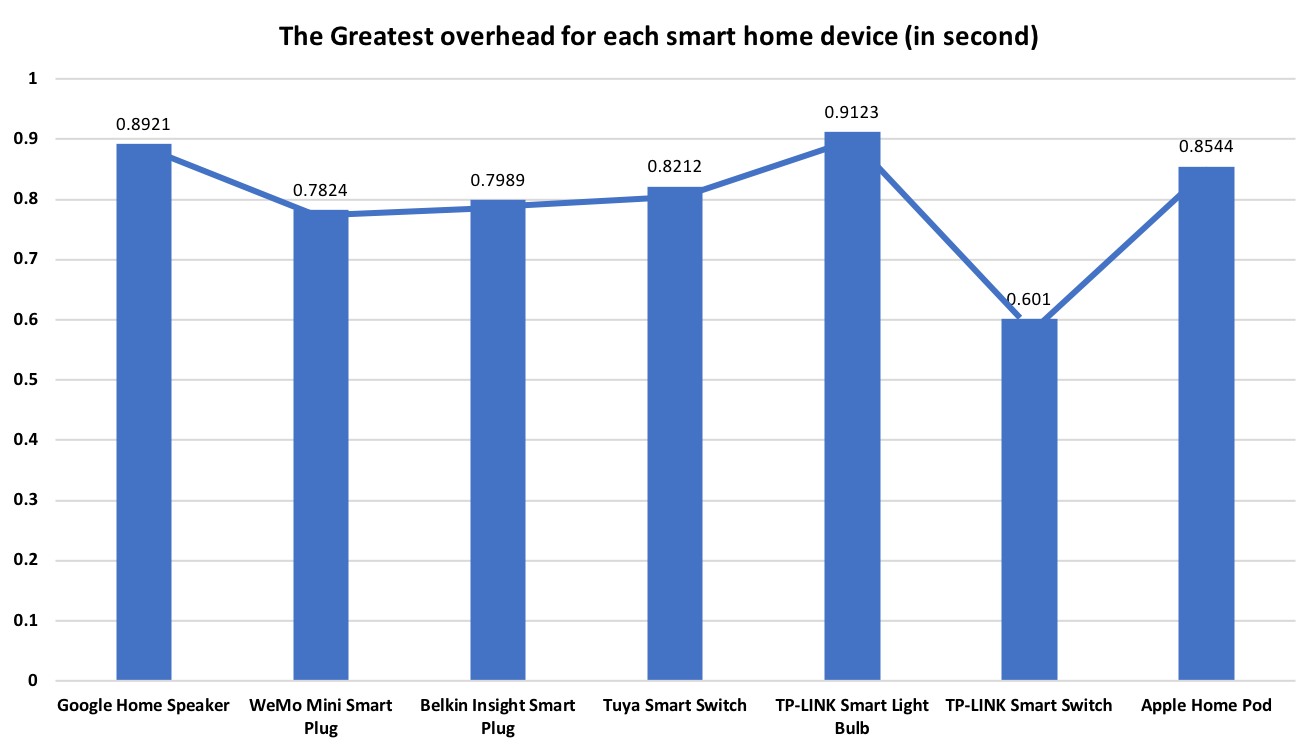
\includegraphics[width=0.9\textwidth]{overhead.png}
        \caption{The largest overhead in time for each smart home device.}
        \label{fig:overhead}
\end{figure*}

Similarly, we collected the running times of the 600 attack trials to analyze the overheads of Mirai and its variants. As a result, the average overheads for Mirai, Satori, and IoT\_reaper are 0.4851 seconds, 0.4312 seconds, and 0.5201 seconds, respectively.

\textbf{Attacks on SmartApps.} 
For the open-port attacks, we collected the running times of the 5,480 trials and found that the average overheads for the first and second attack are 0.838 seconds and 0.801 seconds, respectively. For the overprivilege attacks, the average running time of defending against the 68 attacks are 0.7332 seconds. The reason of the higher averaged processing times for the experiments on SmartApps compared to those for the real-world smart home system lies in that SSL/TLS encryption/decryption and MITM hijacking need longer processing times, which are involved in the analysis on SmartApps.

As one can see from the results, our CLAF implementation imposes a low overhead of less than 1 second in average. 

\subsection{Related Works}
\label{subsec:claf-related}
In this section, we summarize the most-related previous research.

\indent\textbf{Permission Model Design.} The design of permission models plays an important role in securing modern IoT systems and has received much attention in recent years. Jia \emph{et al.}~\cite{jia2017contexiot} proposed a context-based permission model for appified IoT platforms, which requires a patch to the app during installation. %With the definition they concluded and analyzed from the past context researchers, they built their well-defined context model. 
A context is defined as the set of information that is essential to distinguish an attack from a benign logic in an app at runtime. By training a context model based on the past history context of sensitive actions, the proposed permission model can provide contextual integrity of the IoT system. Roesner \emph{et al.} \cite{roesner2012user} proposed a user-driven access control system where the user is continuously involved with the permission decision process case-by-case by using access control gadgets. Wijesekera \emph{et al.}~\cite{wijesekera2015android} advocated contextual integrity as the basic form for the future permission model design based on a rigorous user study on Android platforms. Compared to their work, CLAF does not rely on any data collected from the past operation of the system; and it can be deployed without any modification to the source codes of the IoT devices for command integrity protection.

Tian \emph{et al.} in~\cite{tian2017smartauth} presented a user-centric, semantic-based authorization model called SmartAuth, which can identify possible overprivileged apps by matching an app's description (code comments and published documentations) with its implementation based on natural language processing and code analysis. Sikder \emph{et al.} \cite{sikder20176thsense} proposed an intrusion detection system to distinguish the malicious and benign behaviors of the sensors by analyzing the changes in the sensor data for different tasks. By observing the working conditions of the sensors, their work can detect the malicious behaviors through the pre-defined and trained context-aware models. In contrast, the \textit{policies} in our work are defined exclusively by the user, which is more secure and reliable.

\textbf{IoT Security.}
IoT security research has been thriving in recent years. It is mainly centered on two directions: device security and protocol security. Fernandes \emph{et al.}~\cite{fernandes2016security} studied the Samsung's SmartThings platform by considering a dataset of 499 SmartApps and 132 device handlers. They discovered 2 design flaws that lead to the overprivilege problem and found that the SmartThings event subsystem does not sufficiently protect the events that carry sensitive information. By exploiting these design flaws, they developed 5 PoC attacks targetting the SmartThings smart home system.  Costin \emph{et al.}~\cite{costin2014large} managed to unpack and analyze 26,275 embedded system firmware images crawled from the Internet. With static analysis, they discovered a total of 38 previously unknown vulnerabilities in over 693 firmware images. M$\ddot{u}$ller \emph{et al.}~\cite{muller2017sok} conducted a large-scale analysis on the known printer attacks and wrote a prototype software PRET to automatically evaluate 20 printer models and found that all of them are vulnerable to at least one of the known attacks. Fernandes \emph{et al.}~\cite{fernandes2016flowfence} presented a data protection mechanism called FlowFence, which splits the data flow and the related control flow within the app structure. All sensitive data are only available in a sandbox and the trusted sink declassifies the data according to the flow policy. Manos \emph{et al.}~\cite{antonakakis2017understanding} did a comprehensive analysis on Mirai's emergence and evolution. They analyzed how the botnet emerged, what classes of devices were affected, how Mirai variants evolved and competed for vulnerable hosts, and what types of attacks Mirai exploited. Flavio \emph{et al.}~\cite{garcia2016lock} found that the entry systems of most VW Group vehicles maintain a few global master keys, which allow an adversary to clone a remote control and gain unauthorized access to a vehicle. Celik \emph{et al.}~\cite{celik2018saint} proposed a novel sensitive information tracking method based on taint tracking to effectively detect the sensitive information leakages in SmartThings market apps. Chen \emph{et al.} presented a fuzzing mechanism which can discover possible memory corruptions in IoT devices even when the firmware is unavailable~\cite{chen2018iotfuzzer}.

There also exists researches targetting the communication protocols of the IoT systems. Ronan \emph{et al.}~\cite{ronen2017iot} discovered a bug in the Touchlink part of the Zigbee Light Link protocol implemented by Philips and compromised the global AES-CCM key used to encrypt and authenticate a new firmware so that an attacker can replace the benign firmware with a malicious one over-the-air. With all these findings they implemented a smart light bulb worm which automatically spreads and controls all the Philips smart lights. Jia \emph{et al.} in \cite{jia2018traffic} analyzed the vulnerabilities of authentication traffics in a typical smart home setting with a Google Home speaker serving as a hub to connect IoT devices such as smart bulbs.  Their results reveal 6 vulnerabilities, which lead to 6 attacks that can be easily reproduced by attackers with little knowledge of IoT.

Our CLAF framework targets protecting the smart home systems that may suffer from the open port and overprivilege problems. Our implementation can successfully counter against the popular attacks in practice, as verified by the experimental studies reported in Section~\ref{sec:eval}.

%==========================================================================================================================
\section{Conclusion and Future Work}\label{sec:conclusion}
In this dissertation, we mainly studied the security of Android smartphones from the perspective of system design flaw and from the perspective of side-channel information exploit. More specifically, we study the design flaw of Android Task Mechanism resulting in privilege leakage, and the public side-channel system states which lead to uncovering of a user's social network identities. We also conducted studies on current security and privacy issues of the typical smart home systems. To mitigate the security challenges faced by the smart home systems, we proposed a credential-less authentication framework (CLAF) for the smart home systems.

Our future research will focus more on studying security and privacy for other smart devices and their corresponding systems, especially smart home devices and smart home systems. We plan to excavate the security vulnerabilities and privacy concerns of the current most popular smart home devices and smart home systems and develop new attack vectors. Afterward, we plan to design defense mechanisms from the operating system level to guarantee the safety and privacy of these smart home devices and systems. 

        \newpage
   \bibliographystyle{abbrv}
   \bibliography{thesis}
\end{document} 